\chapter{Results and Discussion}
\label{ch:Results}
This chapter is dedicated to the presentation of the results obtained from characterised detectors. The quenching resistor measurement is in section \ref{ch:Results:Rq}, the breakdown voltage in section \ref{ch:Results:breakdown voltage}, Noise Classification in section \ref{ch:Results:Noise Classification}, and the gain and PDE in sections \ref{ch:Results:Gain} \& \ref{ch:Results:PDE}.

\section{Quenching resistor}
\label{ch:Results:Rq}
 In this section, the quenching resistor measurements of the FBK and Hamamatsu SiPMs are presented. It has been measured with two different methods: from the IV curve in forward bias (see \ref{ch:experiement methods:IV:Rq IV}) and from the waveform analysis (see \ref{ch:experiement methods:WA:Rq WA}).  
 
\subsection{IV curve method} 
The results for the quenching resistors from the IV curve are shown in Fig. \ref{fig:IV curve linear fit and RQ}. The left plots are the IV curve in forward bias and the linear fits. The fitting range has been chosen from $0.5$ to $-2.3$ V for the FBK as discussed with S.Merzi \cite{StefanoMerzi2023PrivateCommunication}. For the Hamamatsu, the fitting range is the same as in \cite{Girard2018CharacterisationDistributions}.
% kind of IV talk 
The IV measurements shown in Fig. \ref{fig:IV curve linear fit and RQ} showed a very high dependency on the choice of the fitting range because the IV curve is not perfectly linear. 
% channels talk
The distinction between the channels [$0,63$] and [$64,127$] is clearly visible, marked by a certain discontinuity in the middle of the plots. This is due to the dead gap separating the two parts of $64$ channels. 
The \SI{31}{\micro m} has a lower $R_Q$ value in the channels  [$0,63$], which is a behavior opposite to the \SI{16}{\micro m} or \SI{42}{\micro m}, this could be due to a different initial position in the wafer. 
The spread over the mean value of $R_Q$ for each channel can be computed and shown in Table \ref{table:Rq + spread}.
\begin{table}[htbp]
\centering
\begin{tabular}{|c|c|c|c|c|}
\hline
Detector            & H2017         & $16 \mu$m     & $31 \mu$m     & $42 \mu$m     \\ \hline
$<R_Q>$ [k$\Omega$] & $550$         & $436 $        & $444 $       & $503 $ \\ \hline
Spread [\%]         & $7.39$        &  $4.6$        & $4.5$        & $3.3$          \\ \hline
\end{tabular}
\caption{Mean $R_Q$ over the measured channel, and the spread $\frac{max(R_Q)-min(R_Q)}{<R_Q>}$. }
\label{table:Rq + spread}
\end{table}
Nevertheless, the discrepancies in the $R_Q$ values are less than $5\%$ for the FBK, which is acceptable. 
% odd and even talk H2017 IV
The hamamatsu H2017 measurement shows a clear difference of $R_Q$ between the odd and even channels, causing a higher spread. Differences in design between FBK and Hamamatsu are responsible for this distinction between odd and even channel that are present in Hamamatsu but not in FBK.


\newgeometry{left=2.2cm,right=2.2cm,top=2cm,bottom=2cm}
\begin{figure}[htbp]
  \centering
  \begin{subfigure}{0.48\textwidth}
    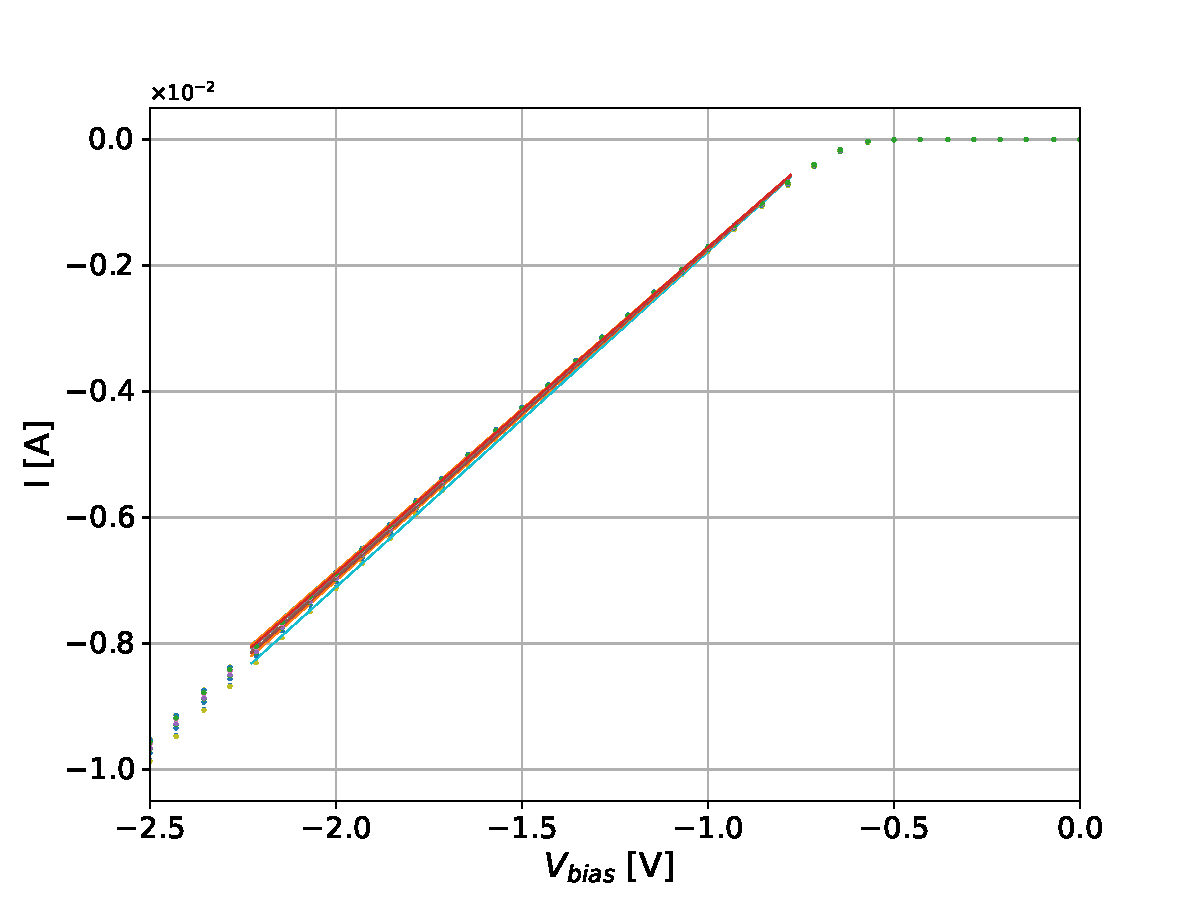
\includegraphics[width=\textwidth]{gfx/plots/Rq/16/FBK_16um_IV.pdf}
    \caption{IV curve linear fit \SI{16}{\micro m}.}
    \label{fig:}
  \end{subfigure}
  \hfill
  \begin{subfigure}{0.48\textwidth}
    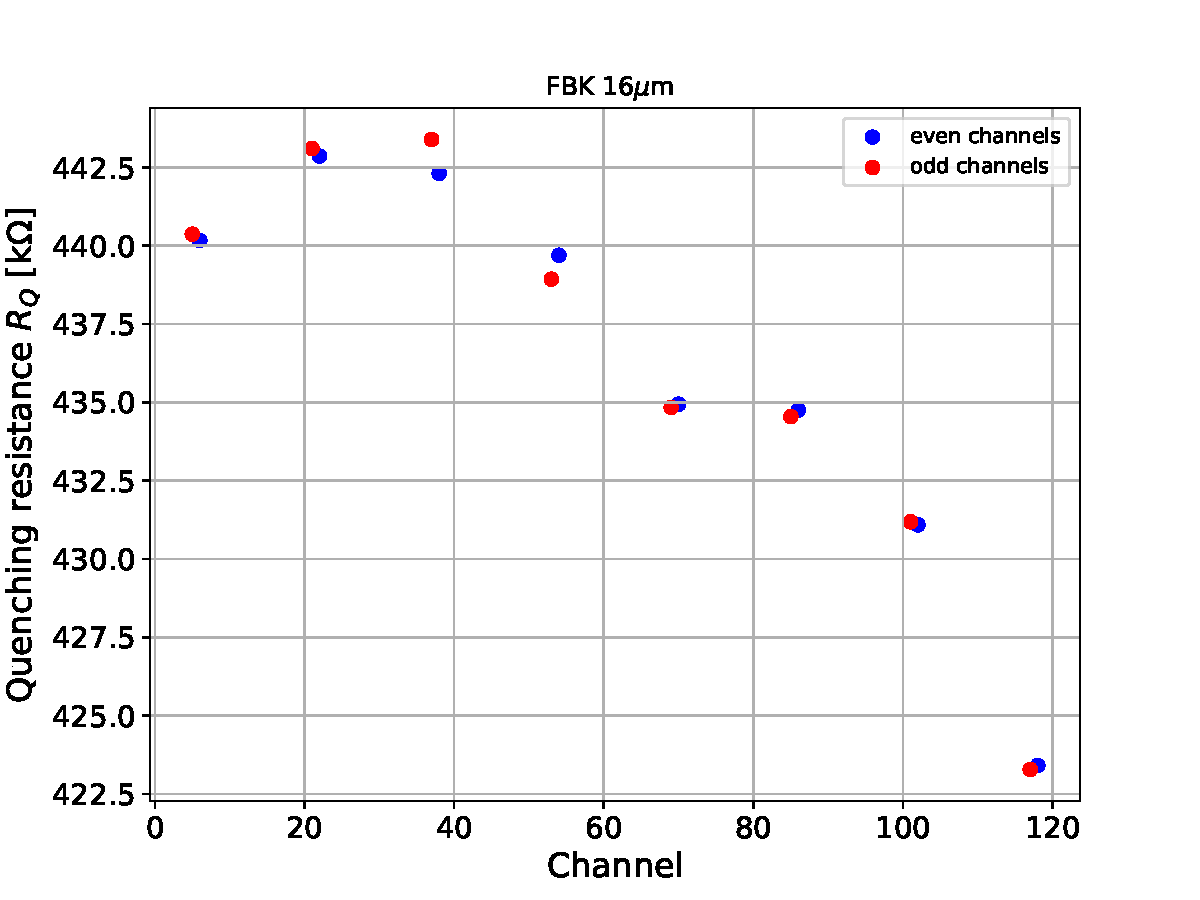
\includegraphics[width=\textwidth]{gfx/plots/Rq/16/FBK_16um_RQs.pdf}
    \caption{$R_Q$ results for \SI{16}{\micro m}.}
    \label{fig:}
  \end{subfigure}
  \begin{subfigure}{0.48\textwidth}
    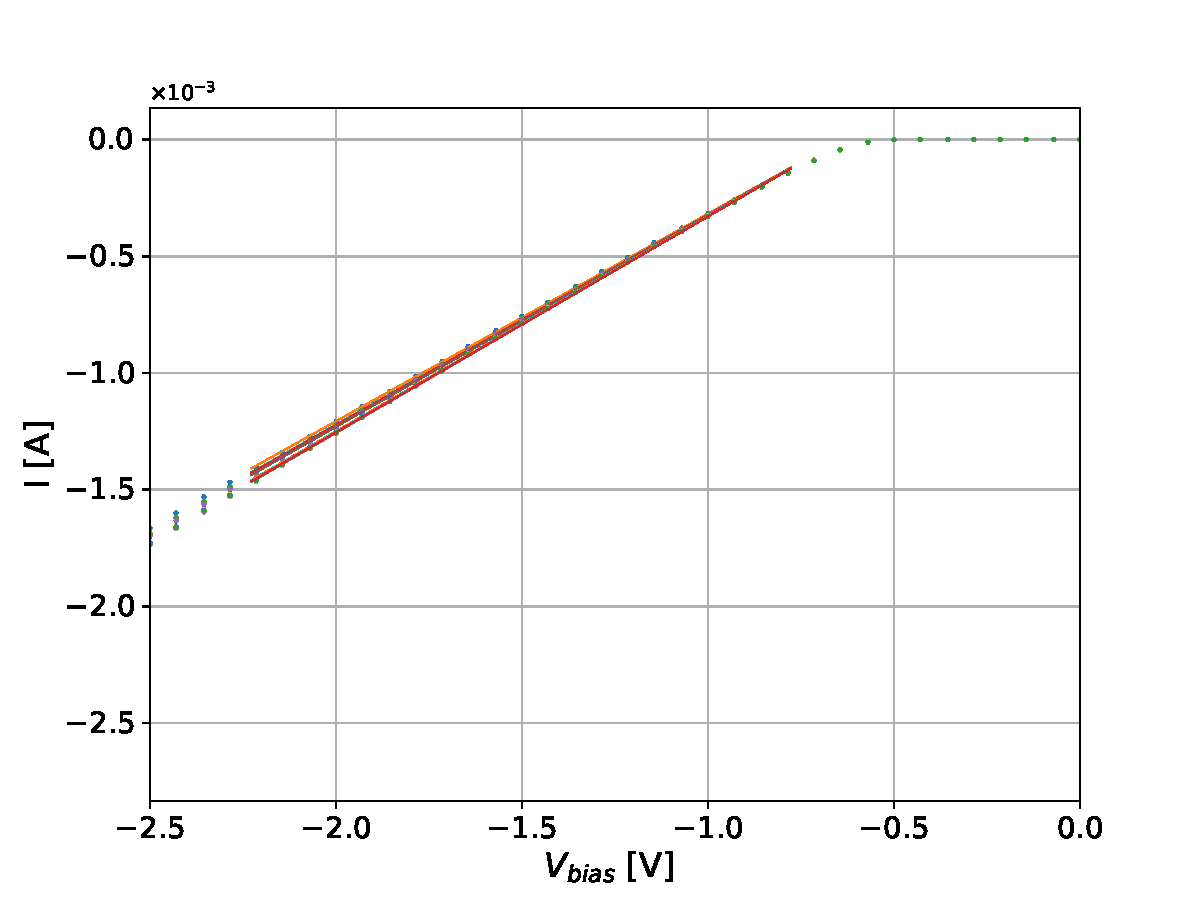
\includegraphics[width=\textwidth]{gfx/plots/Rq/31/FBK_31um_IV.pdf}
    \caption{IV curve linear fit \SI{31}{\micro m}.}
    \label{fig:}
  \end{subfigure}
  \hfill
  \begin{subfigure}{0.48\textwidth}
    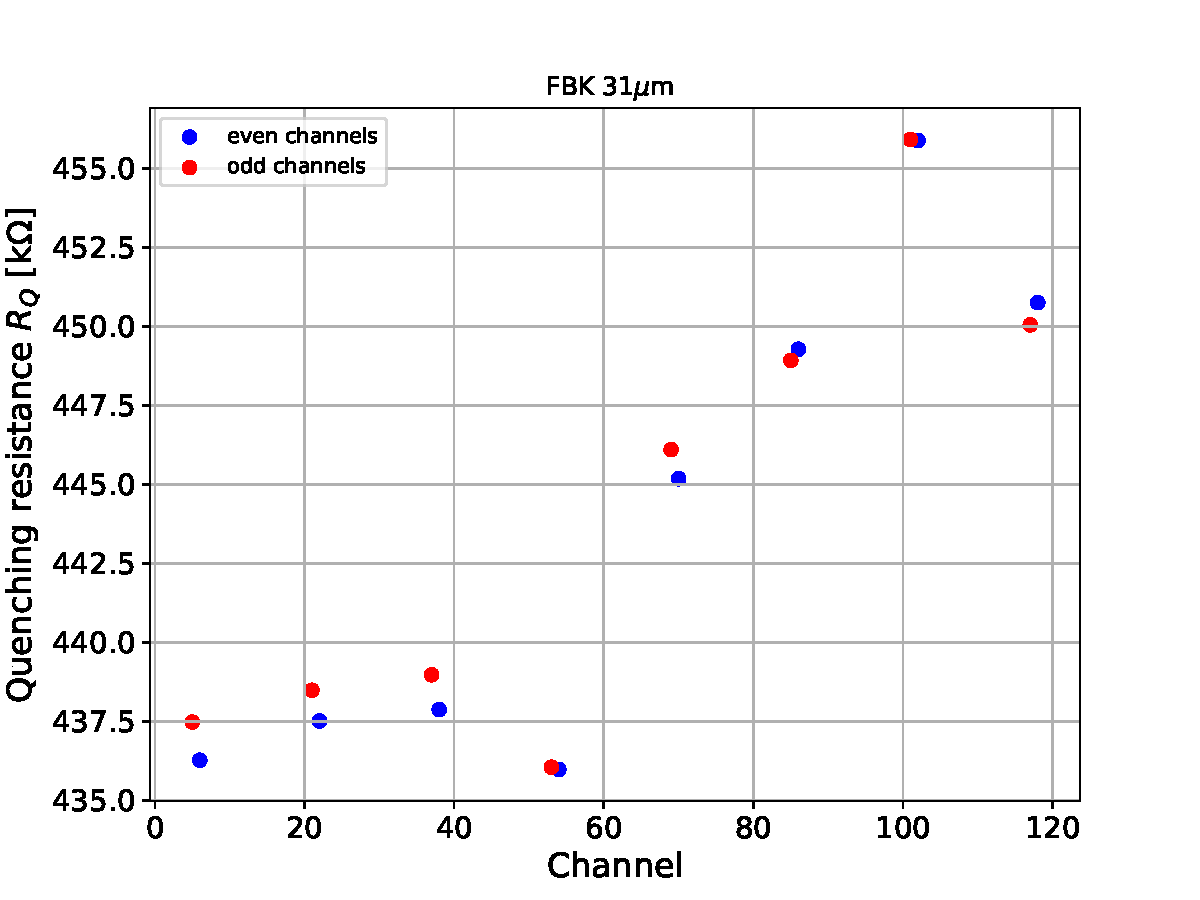
\includegraphics[width=\textwidth]{gfx/plots/Rq/31/FBK_31um_RQs.pdf}
    \caption{$R_Q$ results for \SI{31}{\micro m}.}
    \label{fig:}
  \end{subfigure}
  \begin{subfigure}{0.48\textwidth}
    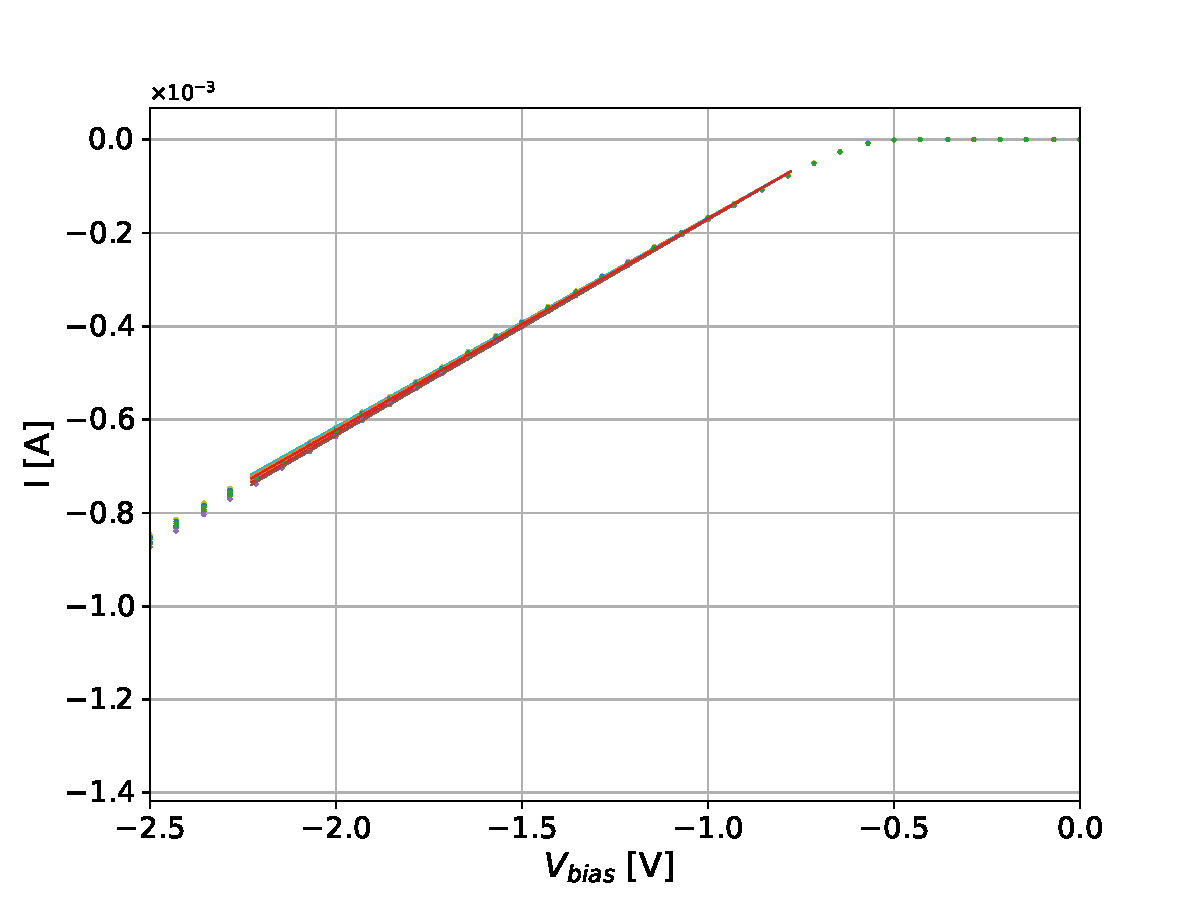
\includegraphics[width=\textwidth]{gfx/plots/Rq/42/FBK_42um_IV.pdf}
    \caption{IV curve linear fit \SI{42}{\micro m}.}
    \label{fig:}
  \end{subfigure}
  \hfill
  \begin{subfigure}{0.48\textwidth}
    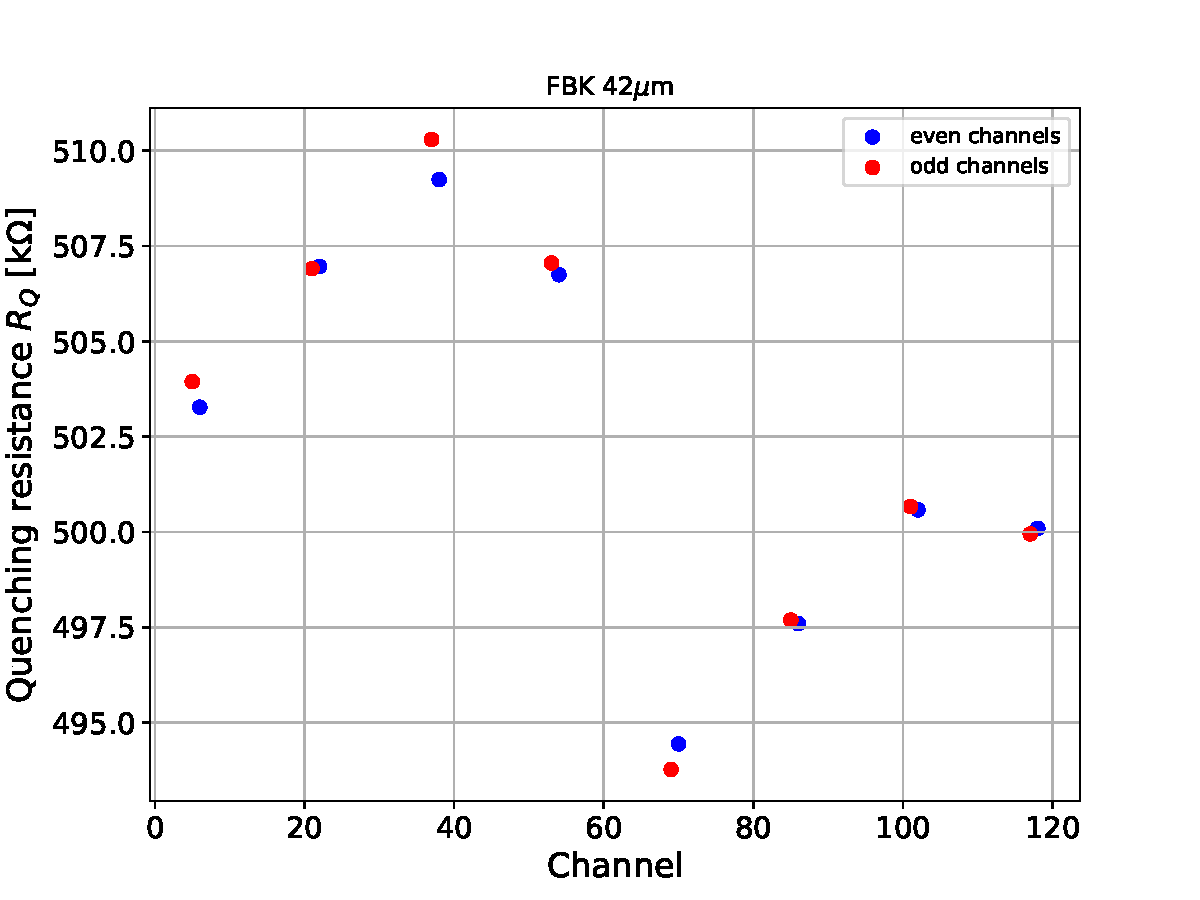
\includegraphics[width=\textwidth]{gfx/plots/Rq/42/FBK_42um_RQs.pdf}
    \caption{$R_Q$ results for \SI{42}{\micro m}.}
    \label{fig:}
  \end{subfigure}
  \begin{subfigure}{0.48\textwidth}
    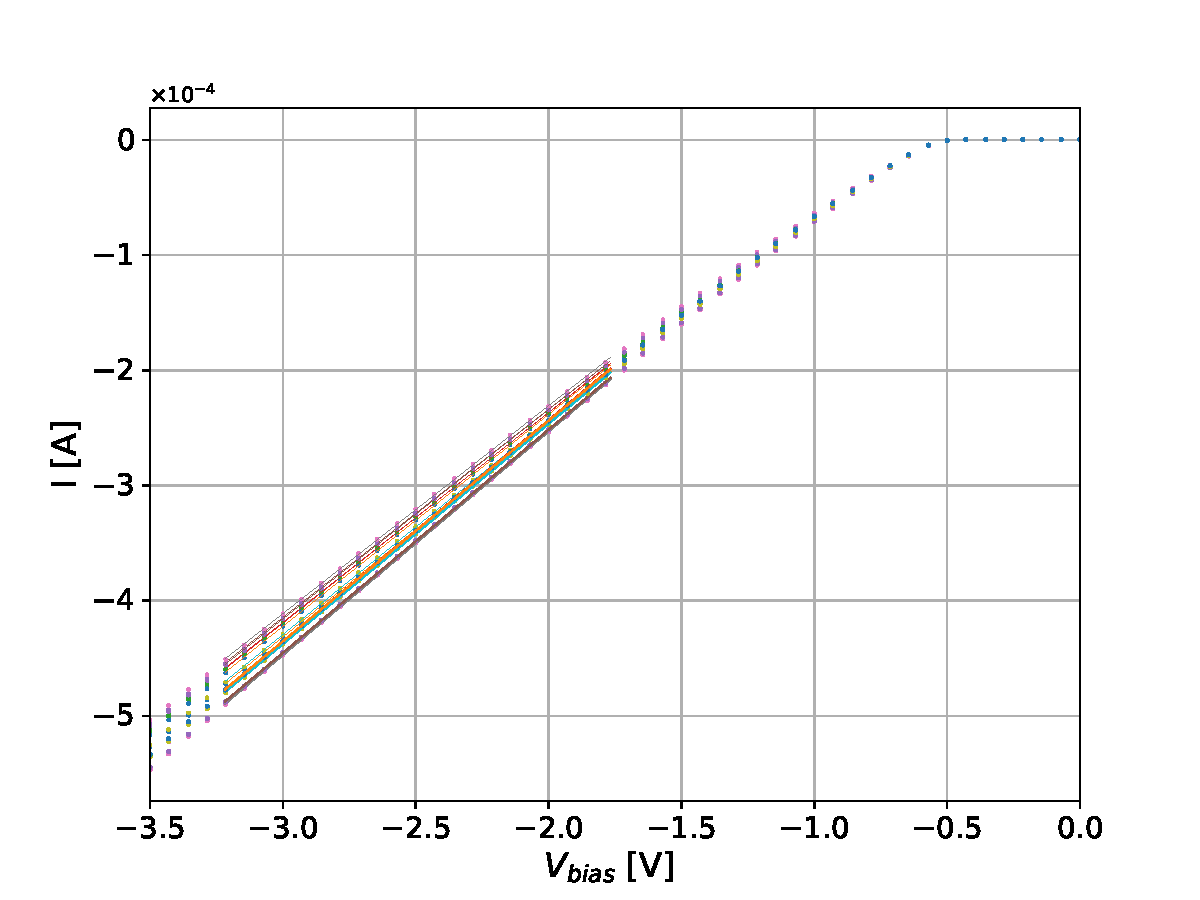
\includegraphics[width=\textwidth]{gfx/plots/Rq/H2017/FBK_2017um_IV.pdf}
    \caption{IV curve linear fit H2017.}
    \label{fig:}
  \end{subfigure}
  \hfill
  \begin{subfigure}{0.48\textwidth}
    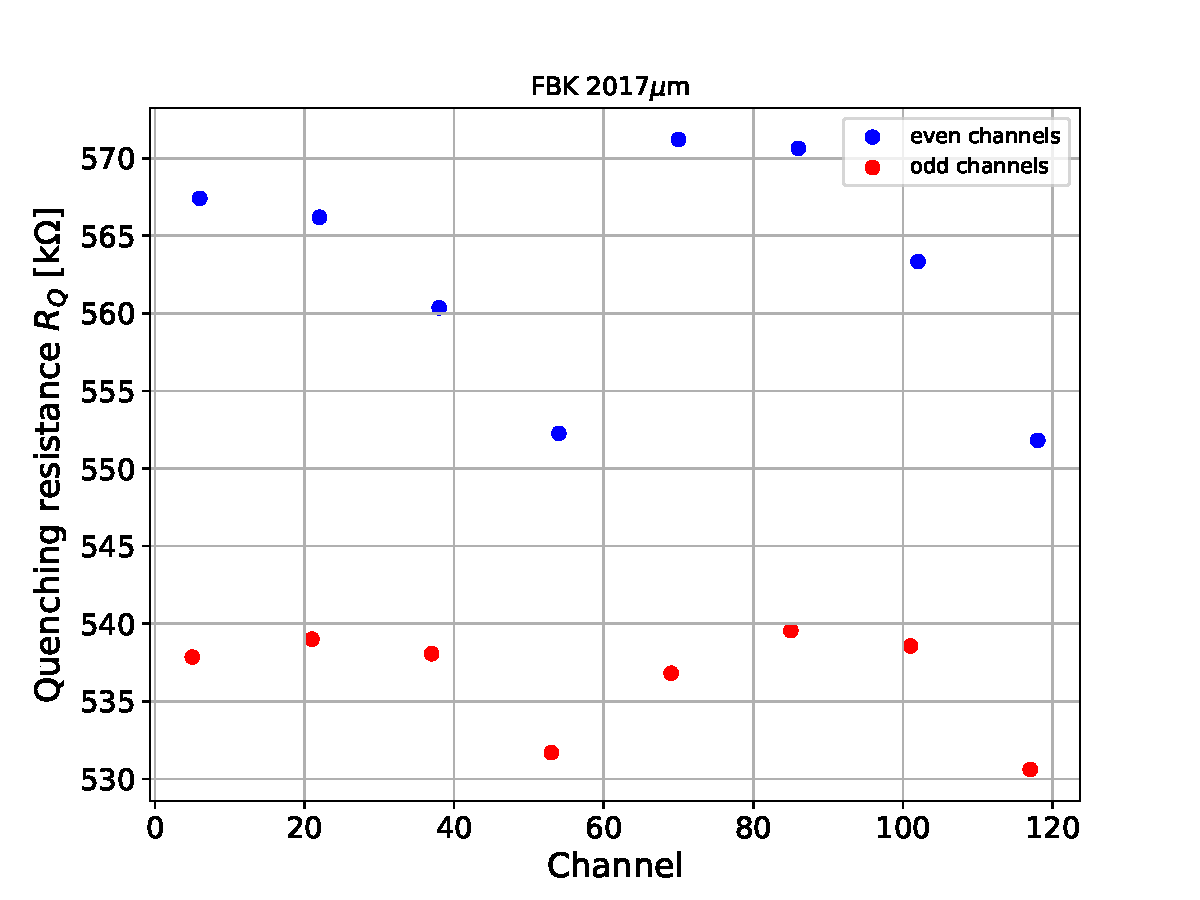
\includegraphics[width=\textwidth]{gfx/plots/Rq/H2017/FBK_2017um_RQs.pdf}
    \caption{$R_Q$ results for H2017.}
    \label{fig:}
  \end{subfigure}
  \caption{Plots of the IV curve fits (left) and the quenching resistor (right) for all detectors.}
  \label{fig:IV curve linear fit and RQ}
  
\end{figure}

\restoregeometry

\subsection{Time constant method}
 For the time constant methods, the results are shown in Table. \ref{table:taulongs table} and Fig. \ref{fig:tau longs}.
\begin{figure}[htbp]
    \centering
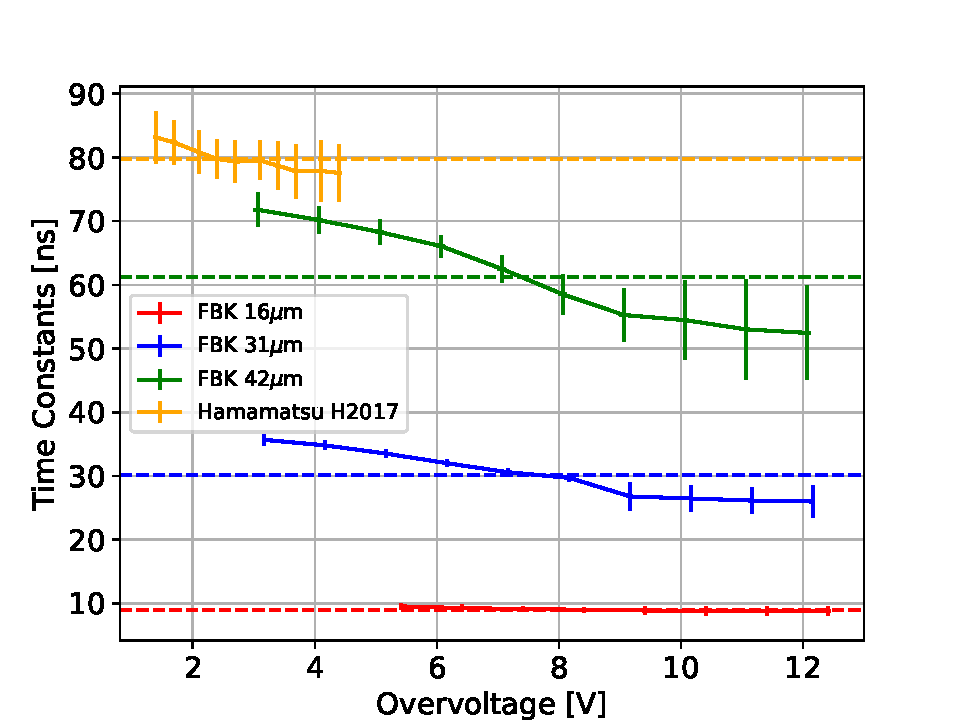
\includegraphics[width=\textwidth]{gfx/plots/WA/taulongs.pdf}
    \caption{$\tau_{long}$ as a function of $\Delta V$ for every detectors.}
    \label{fig:tau longs}
\end{figure}
\begin{table}[htbp]
\begin{tabular}{|c|c|c|c|c|}
\hline
\textbf{}                         & \textbf{FBK \SI{16}{\micro m}} & \textbf{FBK \SI{31}{\micro m} }        & \textbf{FBK \SI{42}{\micro m}} & \textbf{Hamamatsu H2017} \\ \hline
\textbf{$<\tau_{long}>$ {[}ns{]}} & $9 \pm 1.8$         & $30\pm 6$       & $61 \pm 12$        & $79.7 \pm 4$         \\ \hline
%\textbf{$C_d$}                    & $0.227\cdot 10^{-13}$  & $0.708\cdot 10^{-13}$ & $1.128\cdot 10^{-13}$  & $1.637\cdot 10^{-13}$    \\ \hline
\textbf{$R_Q$ {[}k$\Omega${]}}    & $396 \pm 87 $          & $422 \pm 93 $          & $497 \pm 109$           & $487\pm 19$             \\ \hline
\end{tabular}
\caption{$R_Q$ values for each detectors. With $20\%$ errors on $\tau_{long}$ (FBK) \& $2\%$ (for H2017) and $2\%$ errors on gain.}
\label{table:taulongs table}
\end{table}
% 1st results 
% tau long talk 
They were computed by measuring first the $\tau_{long}$ time constant with the waveform analysis. On Fig. \ref{fig:tau longs}, the different values as a function of overvoltage is shown for each detectors. A decrease of $\tau_{long}$ as $\Delta V$ increases is observable for all detectors.
In theory, $\tau_{long}$ should be constant, this results in large systematics errors of $20\%$ leading to measurement neither accurate nor satisfying.
%and should be further developed in a future work. 

% 4th comparison with manufacturer and guido. 
% fbk 
The manufacturer (FBK) \cite{StefanoMerzi2023PrivateCommunication} and Hamamatsu states a value of $R_Q = $ \SI{500}{\kilo \ohm}. 
% comparison with lois and guido 
The values for $R_Q$ are not perfectly \SI{500}{\kilo \ohm} due variations in the manufacture. For the FBK and Hamamatsu detectors, the IV measurements matches with the declared values with a spread below $5\%$ for the FBK. 
The measurements done by Loïs Niggli for the FBK detectors %\textbf{18\% span } 
\cite{NiggliLoisSECTIONIrradiation} are also compatible with what has been measured here. Also, the measurement in \cite{Girard2018CharacterisationDistributions} matches with the Hamamatsu too, with differences that can be due to the fact that the samples studied were different. 

% out look 
The measurement were not taken for all the possible channels, but this shows that the two methods presents similar results. The choice of one method to another depends on the aim of the measurement. Measuring with the IV curve allow to get the $\tau_{rec}$ which is equal to $\tau_{long}$. In the other way around, measuring first the $\tau_{long}$ with the waveform analysis leads to $R_Q$. Note that the IV measurement is way more easier to reproduce if the goal is to characterise more channels and having less systematic errors. The time constant method includes large errors from the gain but especially from the measured $\tau_{long}$. One could use the $R_Q$ values from the IV method to estimate the $\tau_{long}$ and compare it to the measured $\tau_{long}$ from the waveform analysis. 


\section{Breakdown Voltage}
\label{ch:Results:breakdown voltage}
This section presents the breakdown voltage measurements. Results are adjusted for a temperature of \SI{25.0}{\celsius}. In the Table. \ref{table:Vbds temp adjusted}, the measurement from the mean pulse amplitude described in \ref{ch:Experimental methods:breakdown voltage} are shown in the column "\textbf{WA}" and the fits are displayed in \ref{appendix:fig:Vbd fits}. One example is presented in Fig. \ref{fig:Vbd 31um chan6}. As comparison, the values from the $V_{bd}$ characterisation setup based on VATA64 taken by Guido Haefeli are shown in the column of the same name. 
\begin{figure}[htbp]
    \centering
    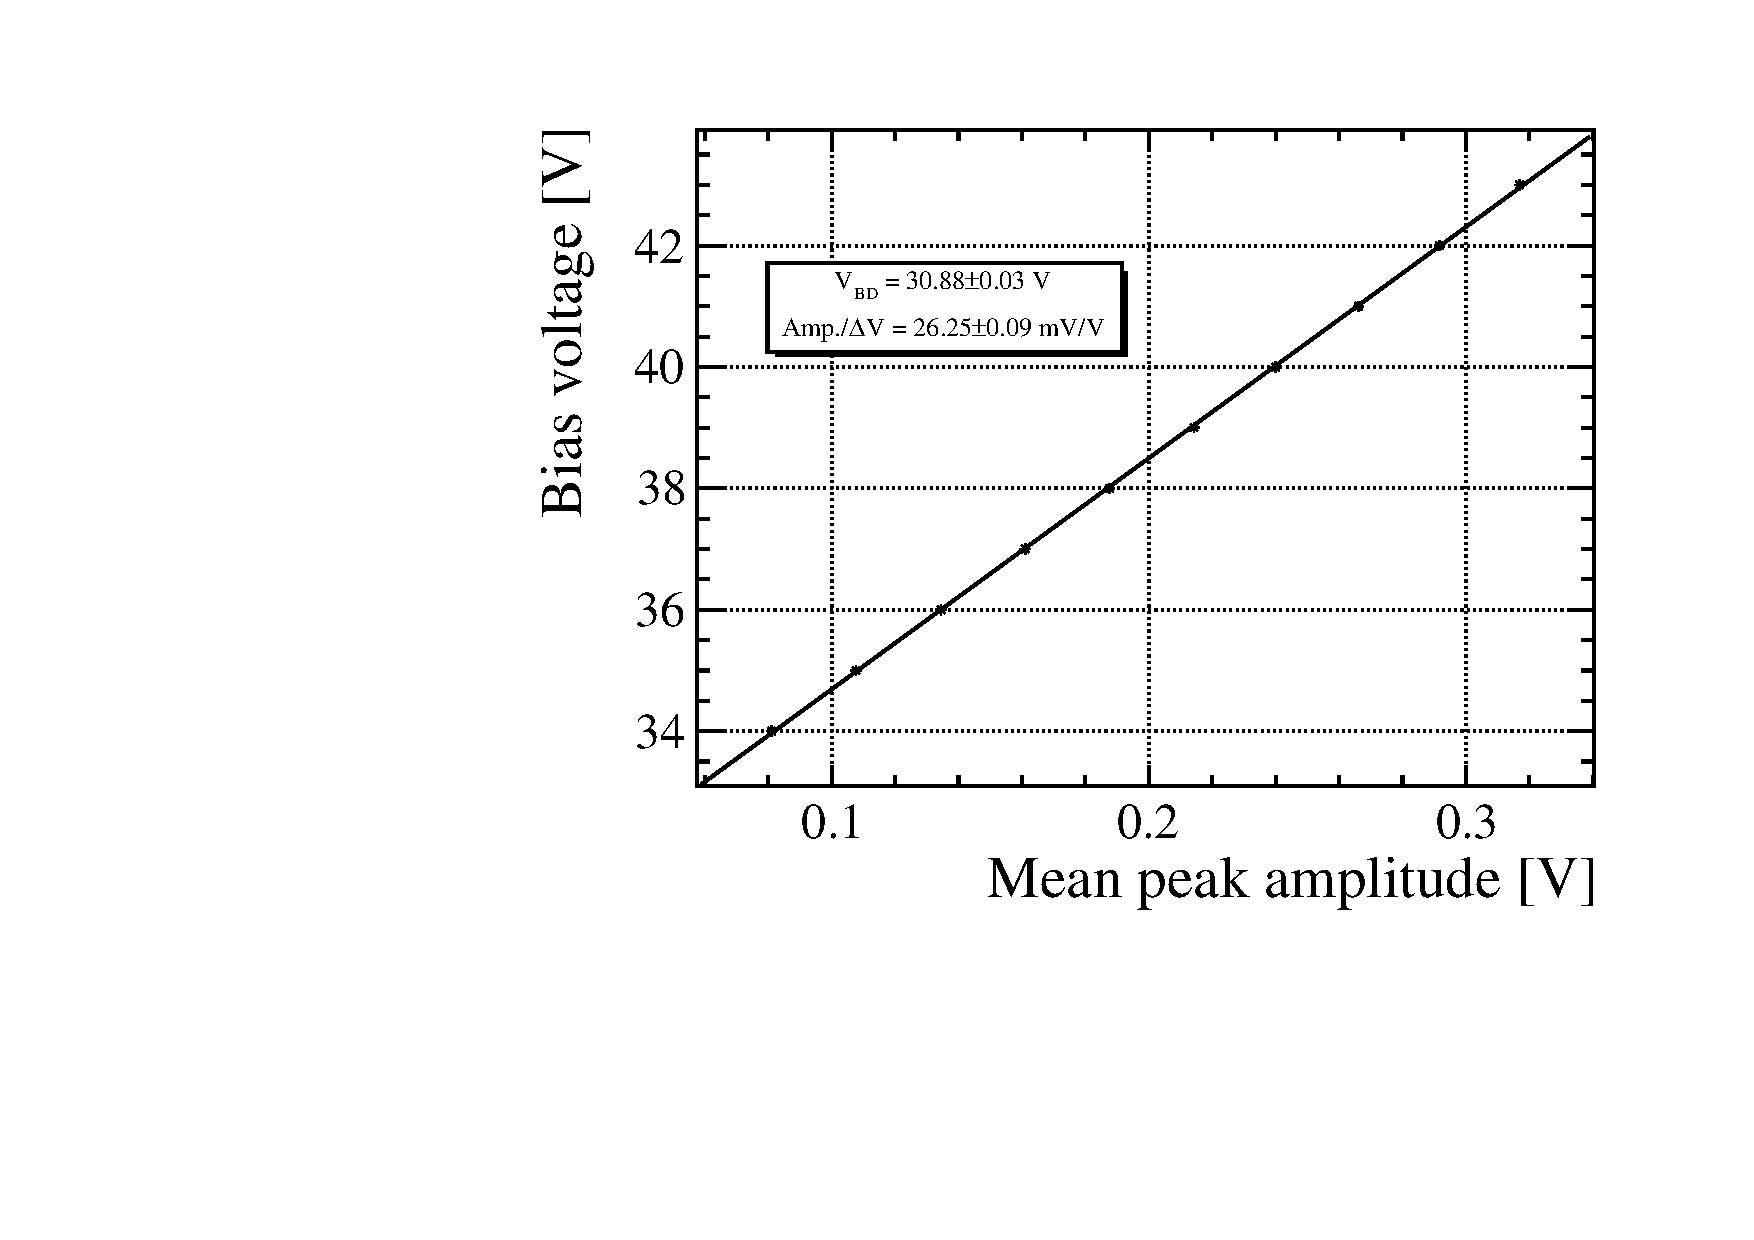
\includegraphics[width=0.7\textwidth]{gfx/plots/WA/31/Breakdown_voltage6.pdf}
    \caption{Breakdown voltage for the FBK \SI{31}{\micro m}, channel $6$.}
    \label{fig:Vbd 31um chan6}
\end{figure}

\begin{figure}[htbp]
  \centering
  \begin{subfigure}{0.48\textwidth}
    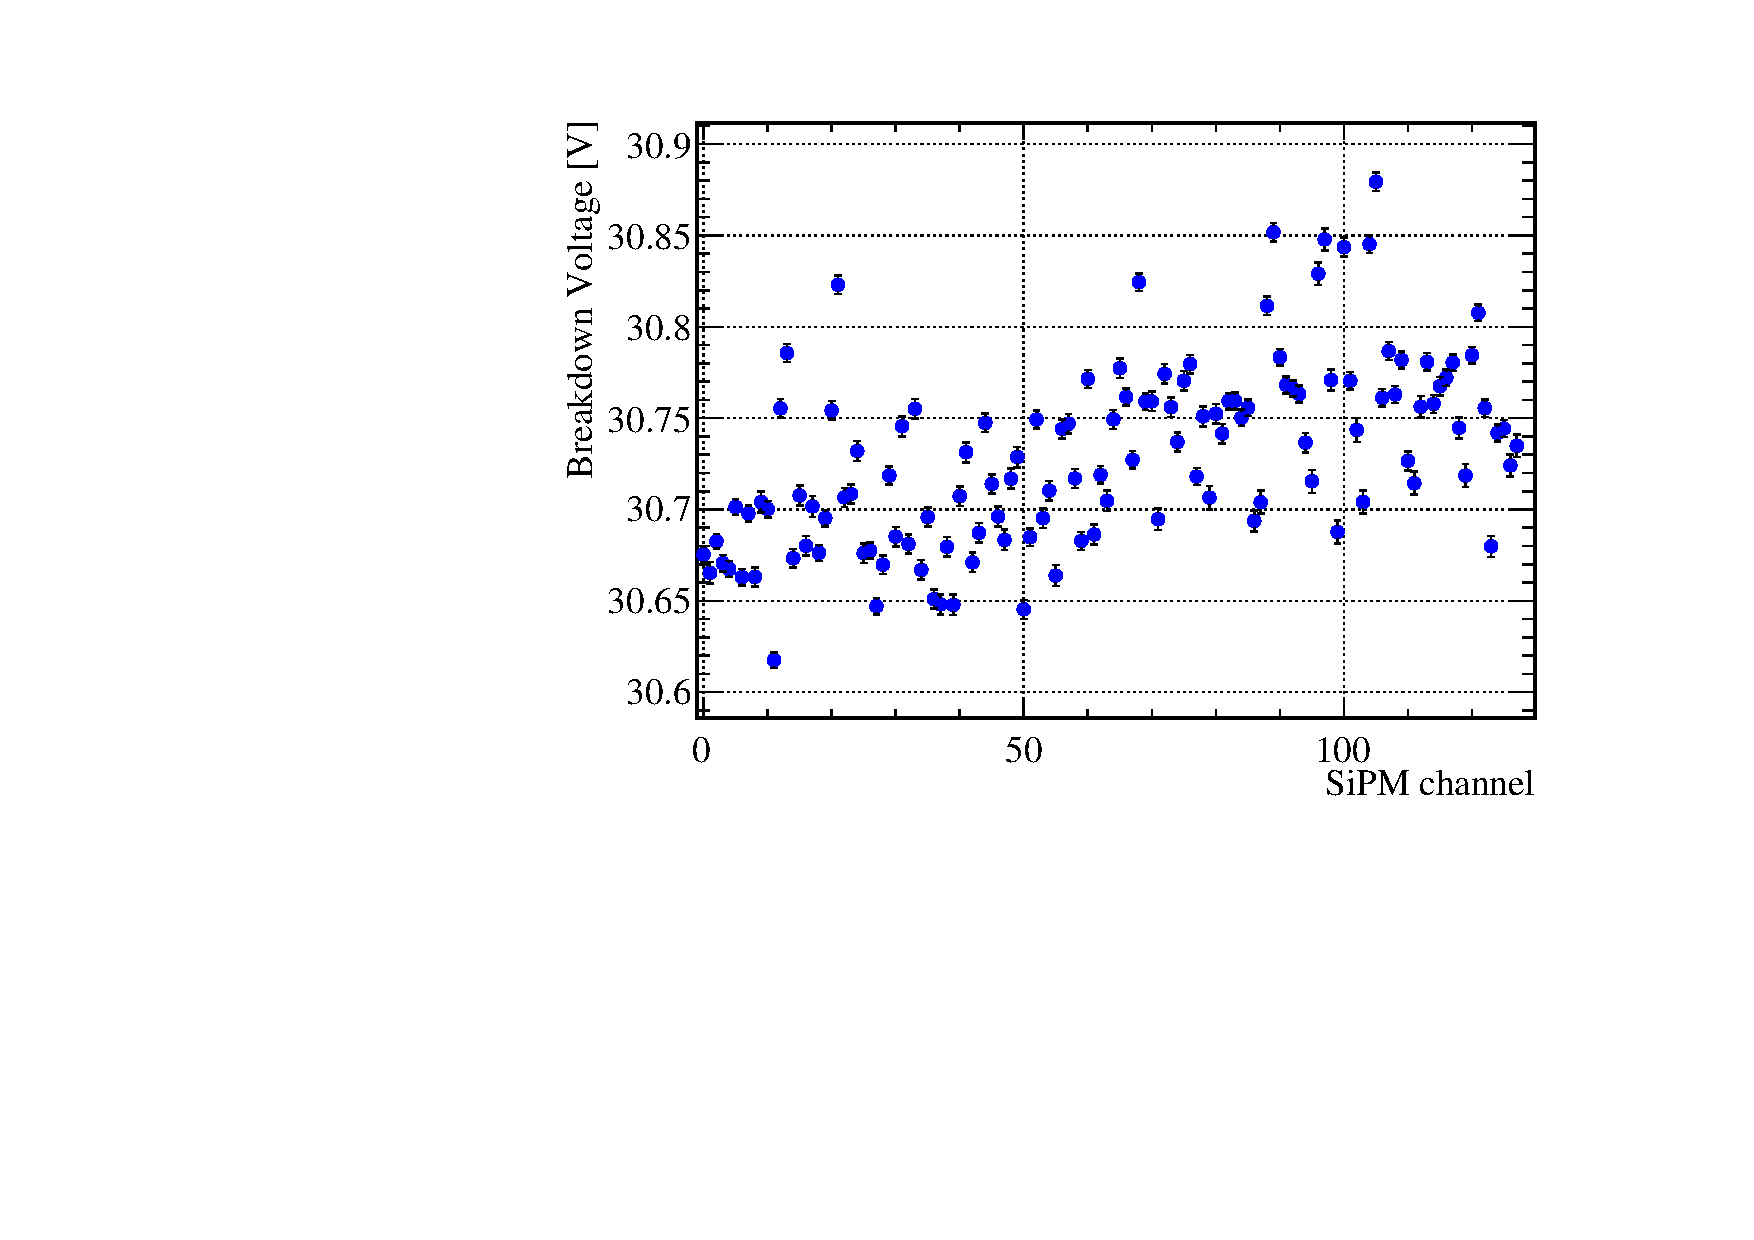
\includegraphics[width=\textwidth]{gfx/plots/WA/16/Vbd16.pdf}
    \caption{$V_{bd}$ \SI{16}{\micro m} sample $12$.}
    \label{fig:}
  \end{subfigure}
  \hfill
  \begin{subfigure}{0.48\textwidth}
    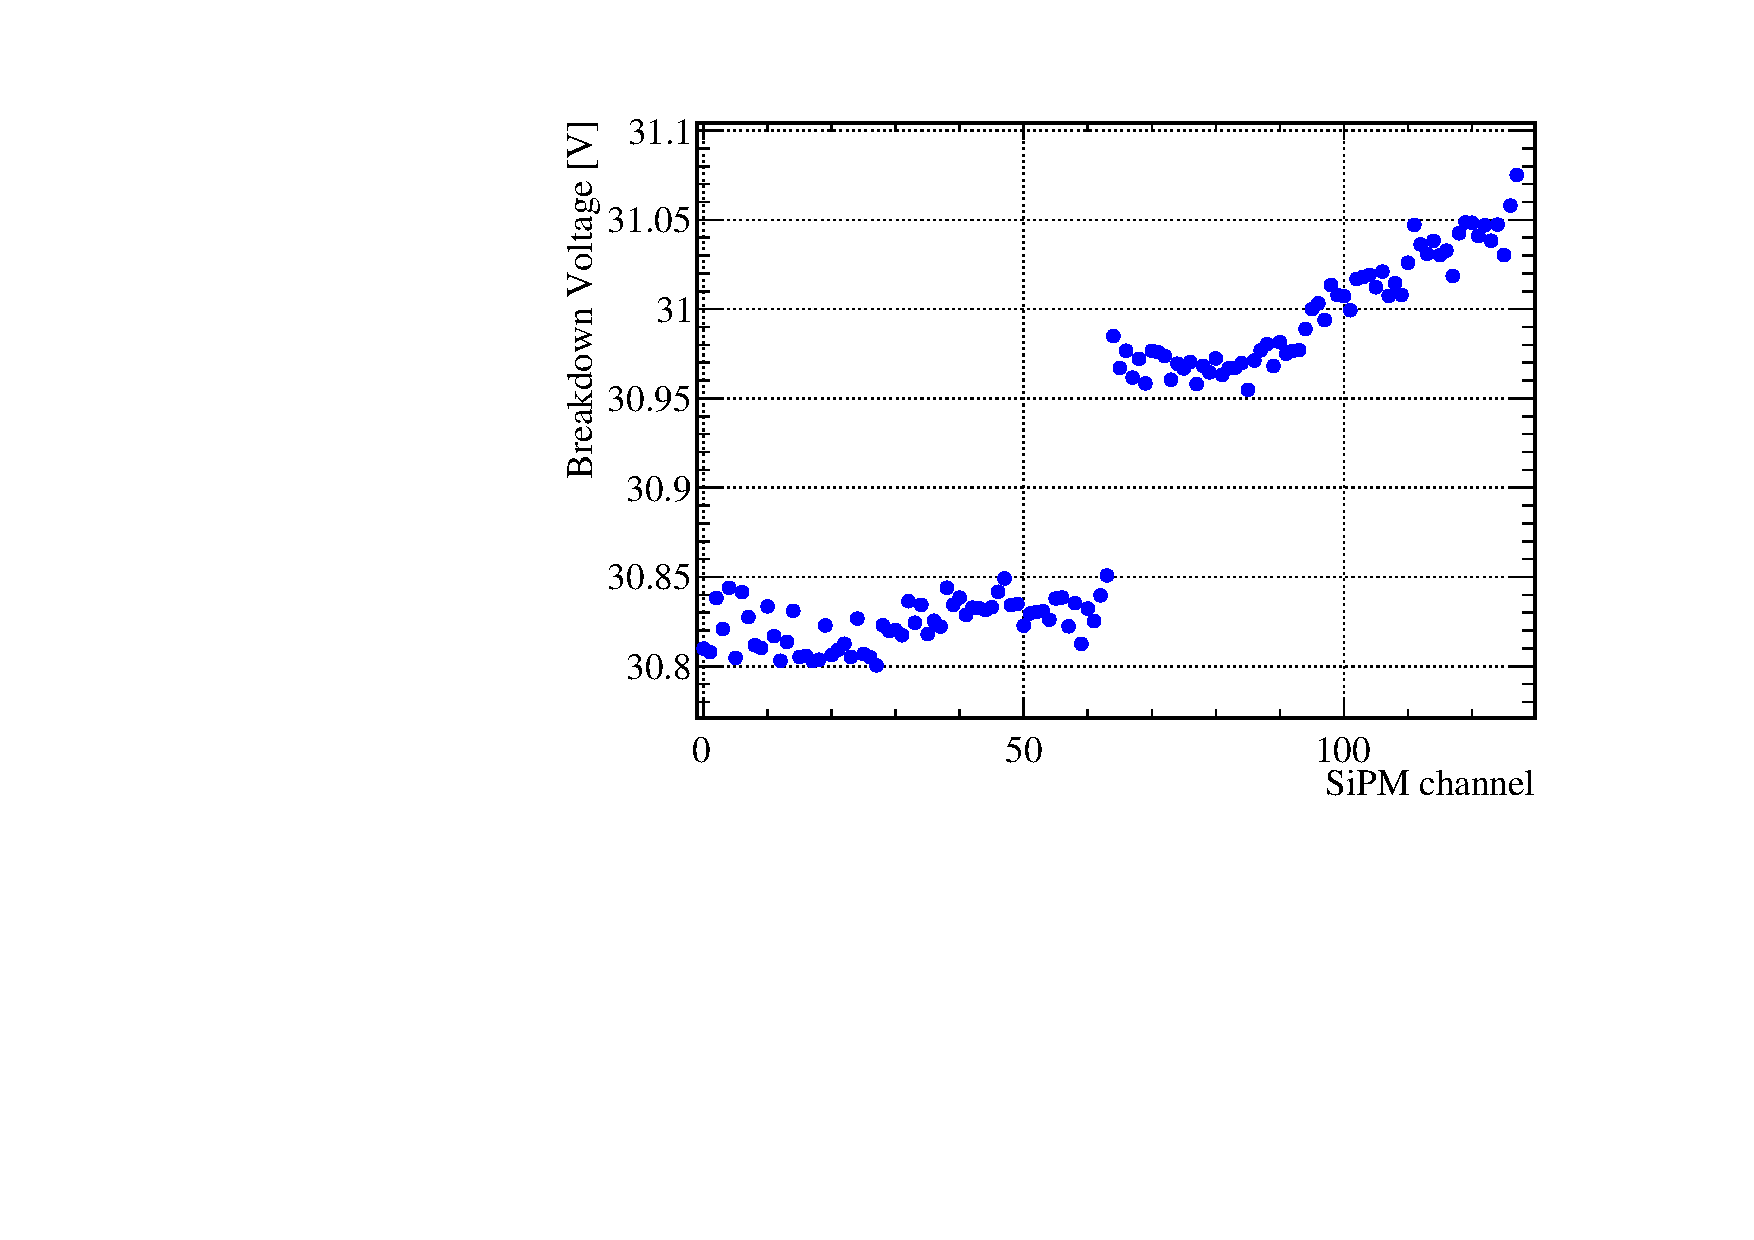
\includegraphics[width=\textwidth]{gfx/plots/WA/31/Vbd31.pdf}
    \caption{$V_{bd}$ \SI{31}{\micro m} sample $6$.}
    \label{fig:}
  \end{subfigure}
  \begin{subfigure}{0.48\textwidth}
    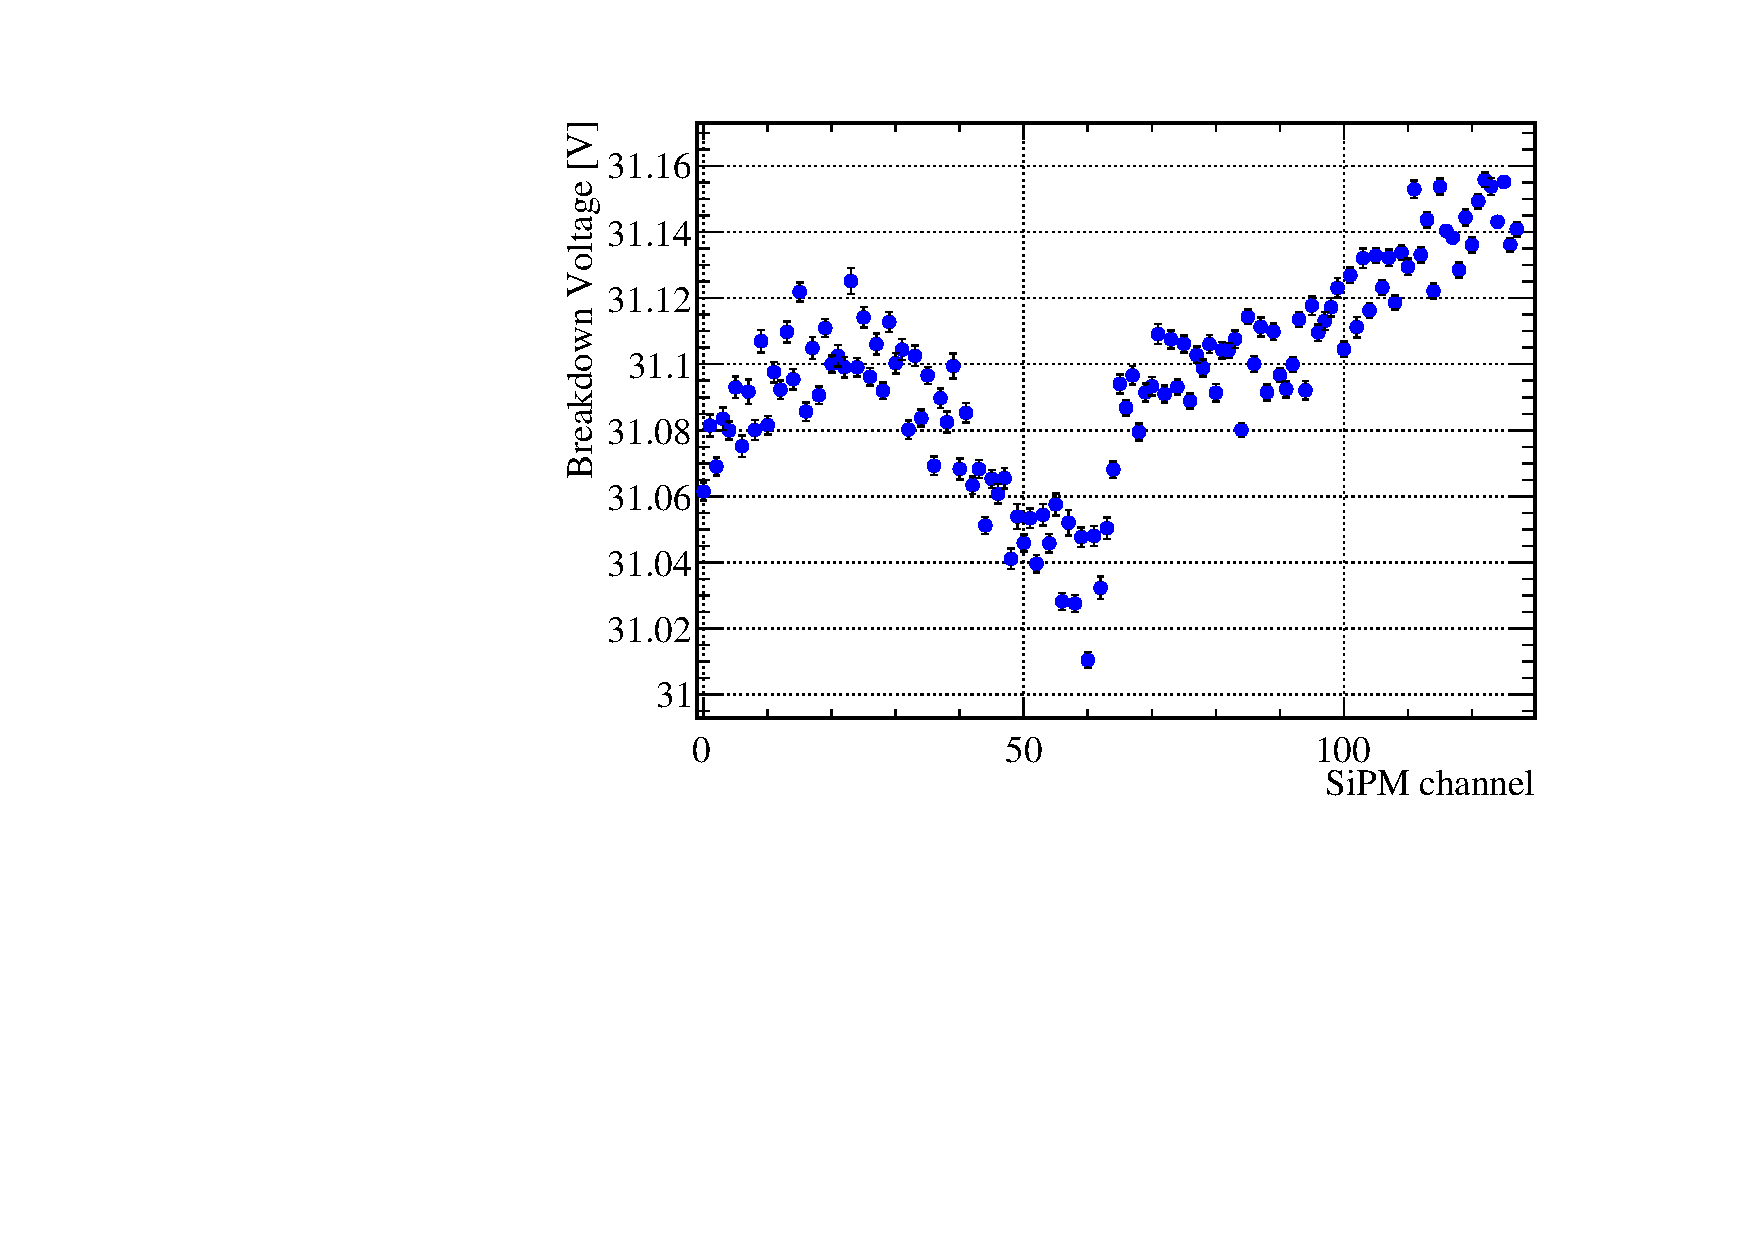
\includegraphics[width=\textwidth]{gfx/plots/WA/42/Vbd42.pdf}
    \caption{$V_{bd}$ \SI{42}{\micro m} sample $1$.}
    \label{fig:}
  \end{subfigure}
  \hfill
  \begin{subfigure}{0.48\textwidth}
    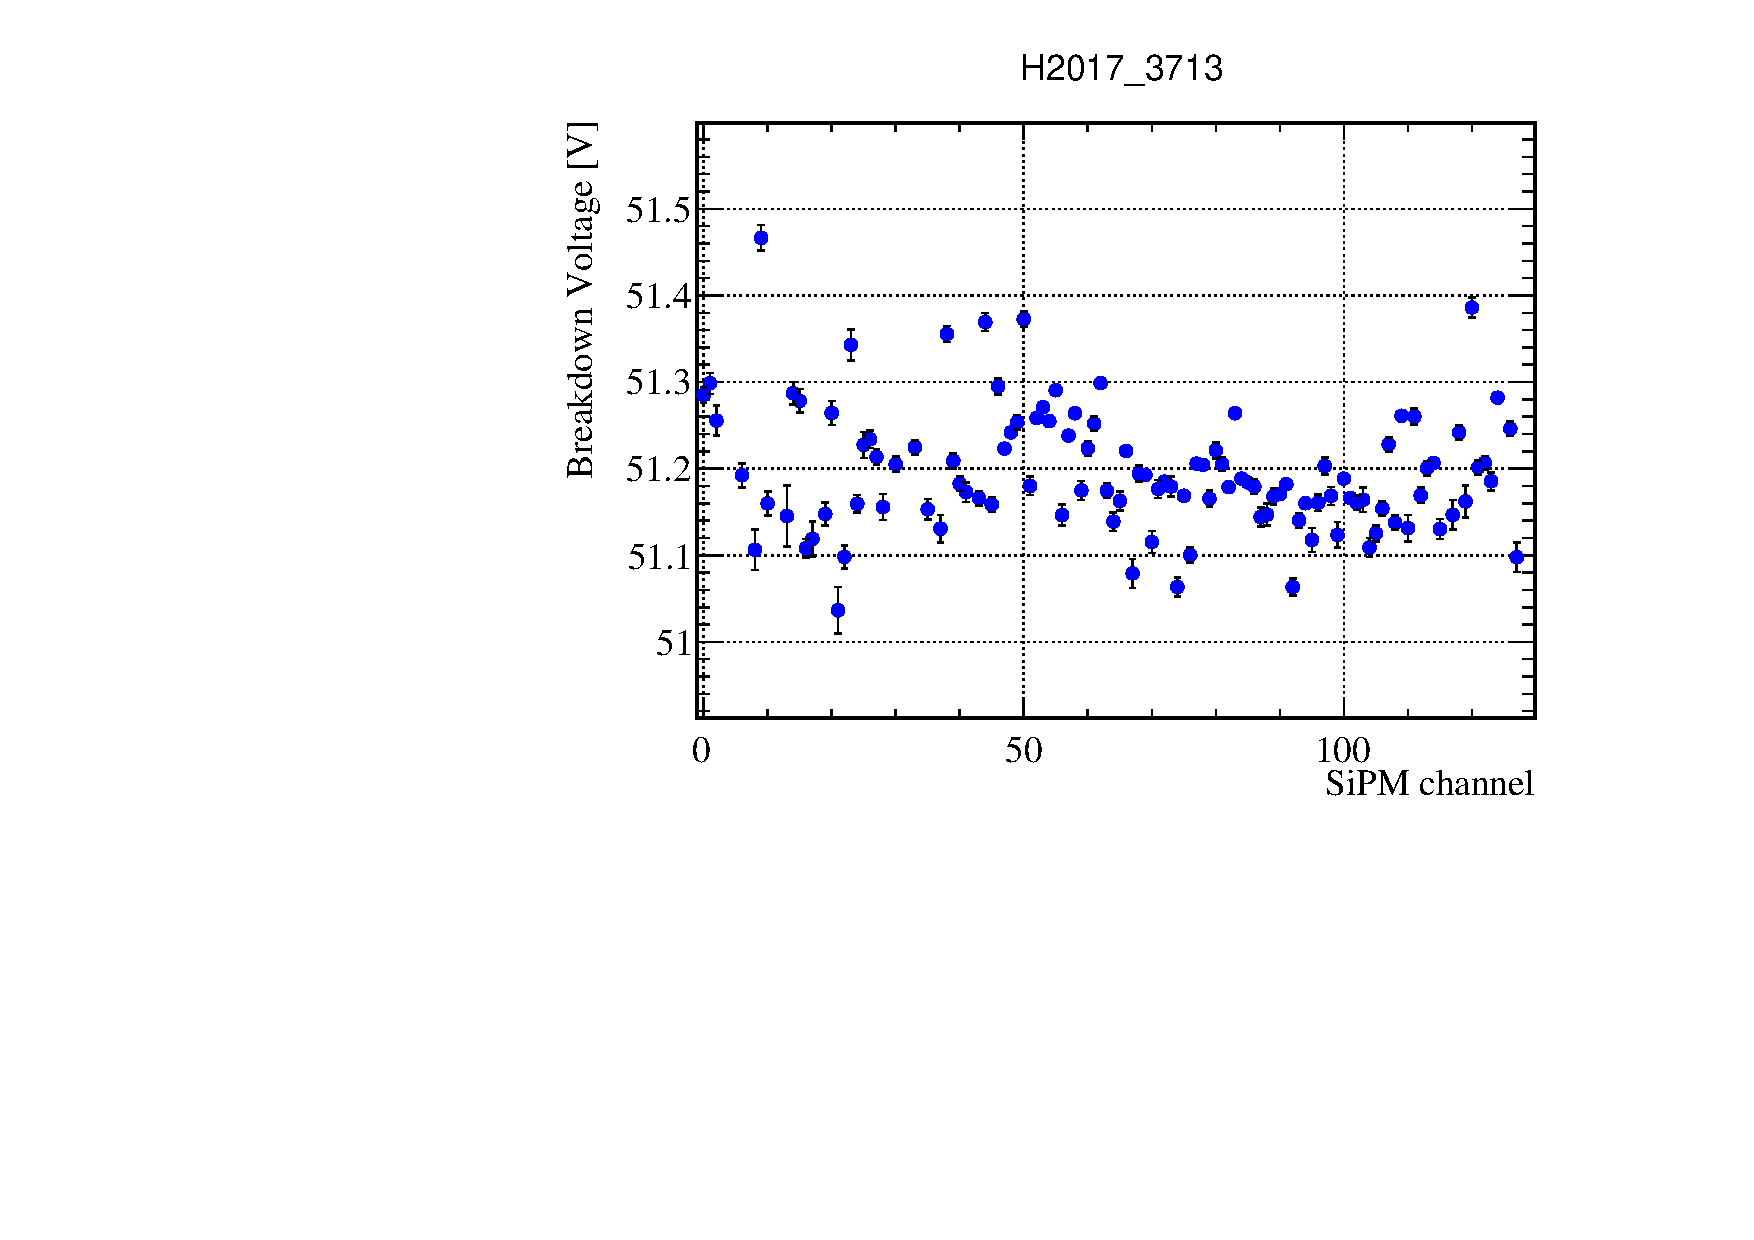
\includegraphics[width=\textwidth]{gfx/plots/WA/H2017/H2016_va64.pdf}
    \caption{$V_{bd}$ H2017.}
    \label{fig:}
  \end{subfigure}
  \caption{Plots of the $V_{bd}$ for all channels (\textbf{VATA64}) for the FBK detectors. }
  \label{fig:Vbd all channels Guido}
\end{figure}

\begin{table}[htbp]
\centering
\begin{tabular}{|c|cc|c|cc|}
\hline
                 & FBK \SI{16}{\micro m}                     & $V_{bd}$ [V] &                  & FBK \SI{31}{\micro m}                    & $V_{bd}$ [V] \\ \cline{2-3} \cline{5-6} 
\textbf{channel} & \multicolumn{1}{c|}{\textbf{WA}} & \textbf{VATA64}  & \textbf{channel} & \multicolumn{1}{c|}{\textbf{WA}} & \textbf{VATA64}  \\ \cline{2-3} \cline{5-6} 
\textbf{70}      & $30.6 \pm 0.3$     & $30.8\pm0.3$   & \textbf{6}       & $30.9\pm0.2$       & $30.9\pm 0.2$     \\
\textbf{86}      & $30.6\pm0.3$       & $30.7\pm 0.3$     & \textbf{36}      & $31.0\pm 0.2$      & $30.8\pm 0.2$     \\ \hline
\textbf{}        & FBK \SI{42}{\micro m}                    & $V_{bd}$ [V] & \textbf{}        & H2017                            & $V_{bd}$ [V] \\ \cline{2-3} \cline{5-6} 
\textbf{channel} & \multicolumn{1}{c|}{\textbf{WA}} & \textbf{VATA64}  & \textbf{channel} & \multicolumn{1}{c|}{\textbf{WA}} & \textbf{VATA64}  \\ \cline{2-3} \cline{5-6} 
\textbf{22}      & $30.9\pm 0.2$      & $31.1\pm 0.2$     & \textbf{54}      & $51.0 \pm 0.2$     &  $51.2\pm 0.2$            \\
\textbf{102}     & $31.0\pm 0.2$      & $31.1 \pm 0.2$      & \textbf{86}      & $51.0 \pm 0.2 $    &  $51.2\pm 0.2$            \\ \hline
\end{tabular}
\caption{$V_{bd}$ corrected with the temperature at \SI{25.0}{\celsius}.}
\label{table:Vbds temp adjusted}
\end{table}

%discussion 

As explained in section \ref{ch:background}, the breakdown voltage value varies from a channel to another and changes as a function of temperature. 
For the WA method, the temperature changed during the measurement. The air conditioner in the lab managed to start the measurement at \SI{25.0}{\celsius} but as overvoltage increases, so did the temperature (up to $26.0-26.5 ^\circ$C). Since this increase of temperature happens for each detectors and at the same amplitudes, the averaged temperature during the measurement is \SI{25.75}{\celsius}. One can then compute the correction associated to this temperature to have the results at \SI{25.0}{\celsius}. As section \ref{ch:background:SiPM:characterised detectors:FBKvsH} tells, the temperature dependency on $V_{bd}$ for the FBK detectors is \SI{32}{\milli V \per \celsius} and \SI{54}{\milli V \per \celsius} for the Hamamatsu. \\
\\
The plots shown in Fig. \ref{fig:Vbd all channels Guido} represent the measured value of $V_{bd}$ for all the channels. The spread in $V_{bd}$ is measured to be $ 0.26$ V, $0.27$V and $0.15$ V for the \SI{16}{\micro m}, \SI{31}{\micro m} and \SI{42}{\micro m} respectively. During the measurement (VATA64), the temperature for the \SI{16}{\micro m} and \SI{31}{\micro m} was \SI{24.7}{\celsius}n \SI{24.6}{\celsius} for the \SI{42}{\micro m} and \SI{25.0}{\celsius} for H2017. 
%The temperature adjustment is then  \SI{9.6}{\milli V} and \SI{12.8}{\milli V} respectively.
These measurements were done by Guido Haefeli and are used as comparison. The measured values (\textbf{WA}) show satisfying results limiting the difference with the \textbf{VATA64} method by less than \SI{200}{\milli V}. 

\section{Noise Classification}
\label{ch:Results:Noise Classification}
% intro 
Finding the correlated noise is necessary to characterize the SiPM. It allows for each detectors to define their operation range and helps in the computation of PDE and gain. Knowing the percentage of DiXT helps to correct measured quantities such as photo-current since DiXT peaks produce more photo-current than a 1 \ac{PE} pulse. But also AP and secondary peaks play a role in the current correction.
The measurement presented in Fig. \ref{fig:correlated noises + epoxy} shows the correlated noise as a function of overvoltage $\Delta V$ for the four FBK detectors, the Hamamatsu H2017. 
\\
The thresholds for classifying the different types of noise have been defined for the H2017, \SI{31}{\micro m} are available on Table \ref{table:thresholds wa}. \SI{16}{\micro m} has the exact same parameters except that the DeXT minimal time is \SI{15.0}{\nano s}. For the \SI{42}{\micro m}, the only change is AP [$ 0.5$, $ 0.85 $[. \SI{31}{\micro m} + epoxy detector had a lot of ringing  and secondary peaks making the classification difficult. To avoid an over correction of the PDE, the DiXT time threshold was increased to \SI{20}{\nano s} and the DeXT amplitude to \SI{0.9}{PE}.

\begin{table}[htbp]
\centering
\begin{tabular}{|c|c|c|c|}
\hline
\textbf{Threshold}      & \textbf{DiXT} & \textbf{DeXT}   & \textbf{AP}     \\ \hline
\textbf{Time [ns]}      & $\leq2.0$     & >$2.0$          & >$15.0$         \\ \hline
\textbf{Amplitude [PE]} & >$1.17$       & ]$ 0.85 $,$ 1.17 $] & [$ 0.6 $, $ 0.85 $[ \\ \hline
\end{tabular}
\caption{Thresholds for the noise classification.}
\label{table:thresholds wa}
\end{table}

To cross check that the thresholds are tuned properly, one can plot the waveform maximal amplitude as a function of their arrival time as in Fig. \ref{fig:peakamptime 42} for the \SI{42}{\micro m}: One can see the different noises, including secondaries than may be just due to misidentification.

\newgeometry{left=1.5cm,right=1.5cm,top=2cm,bottom=2cm}
\begin{figure}[htbp]
  \centering
  \begin{subfigure}{0.48\textwidth}
    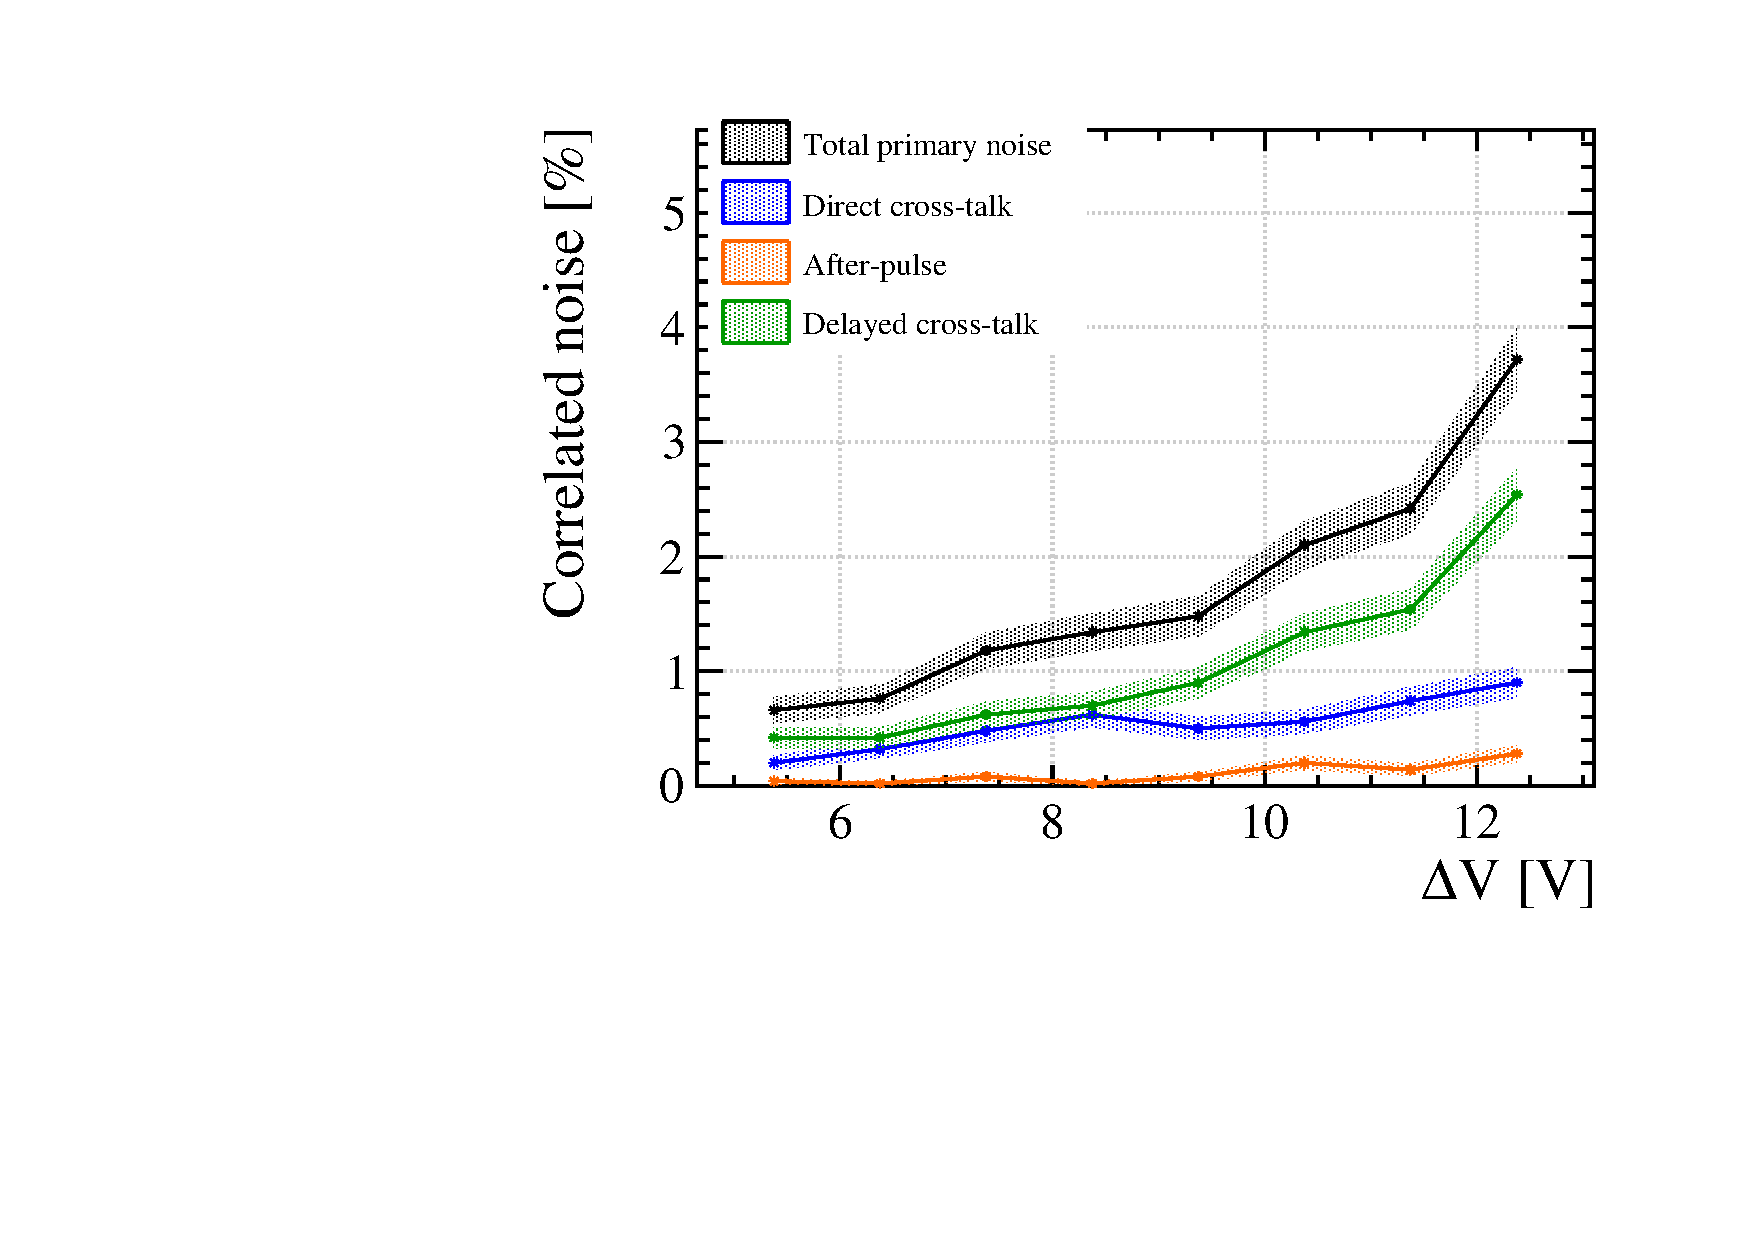
\includegraphics[width=1\linewidth]{gfx/plots/WA/16/CorrelatedNoise.pdf}
    \caption{FBK \SI{16}{\micro m}, channel $70$.}
    \label{fig:}
  \end{subfigure}
  \hfill
  \begin{subfigure}{0.48\textwidth}
    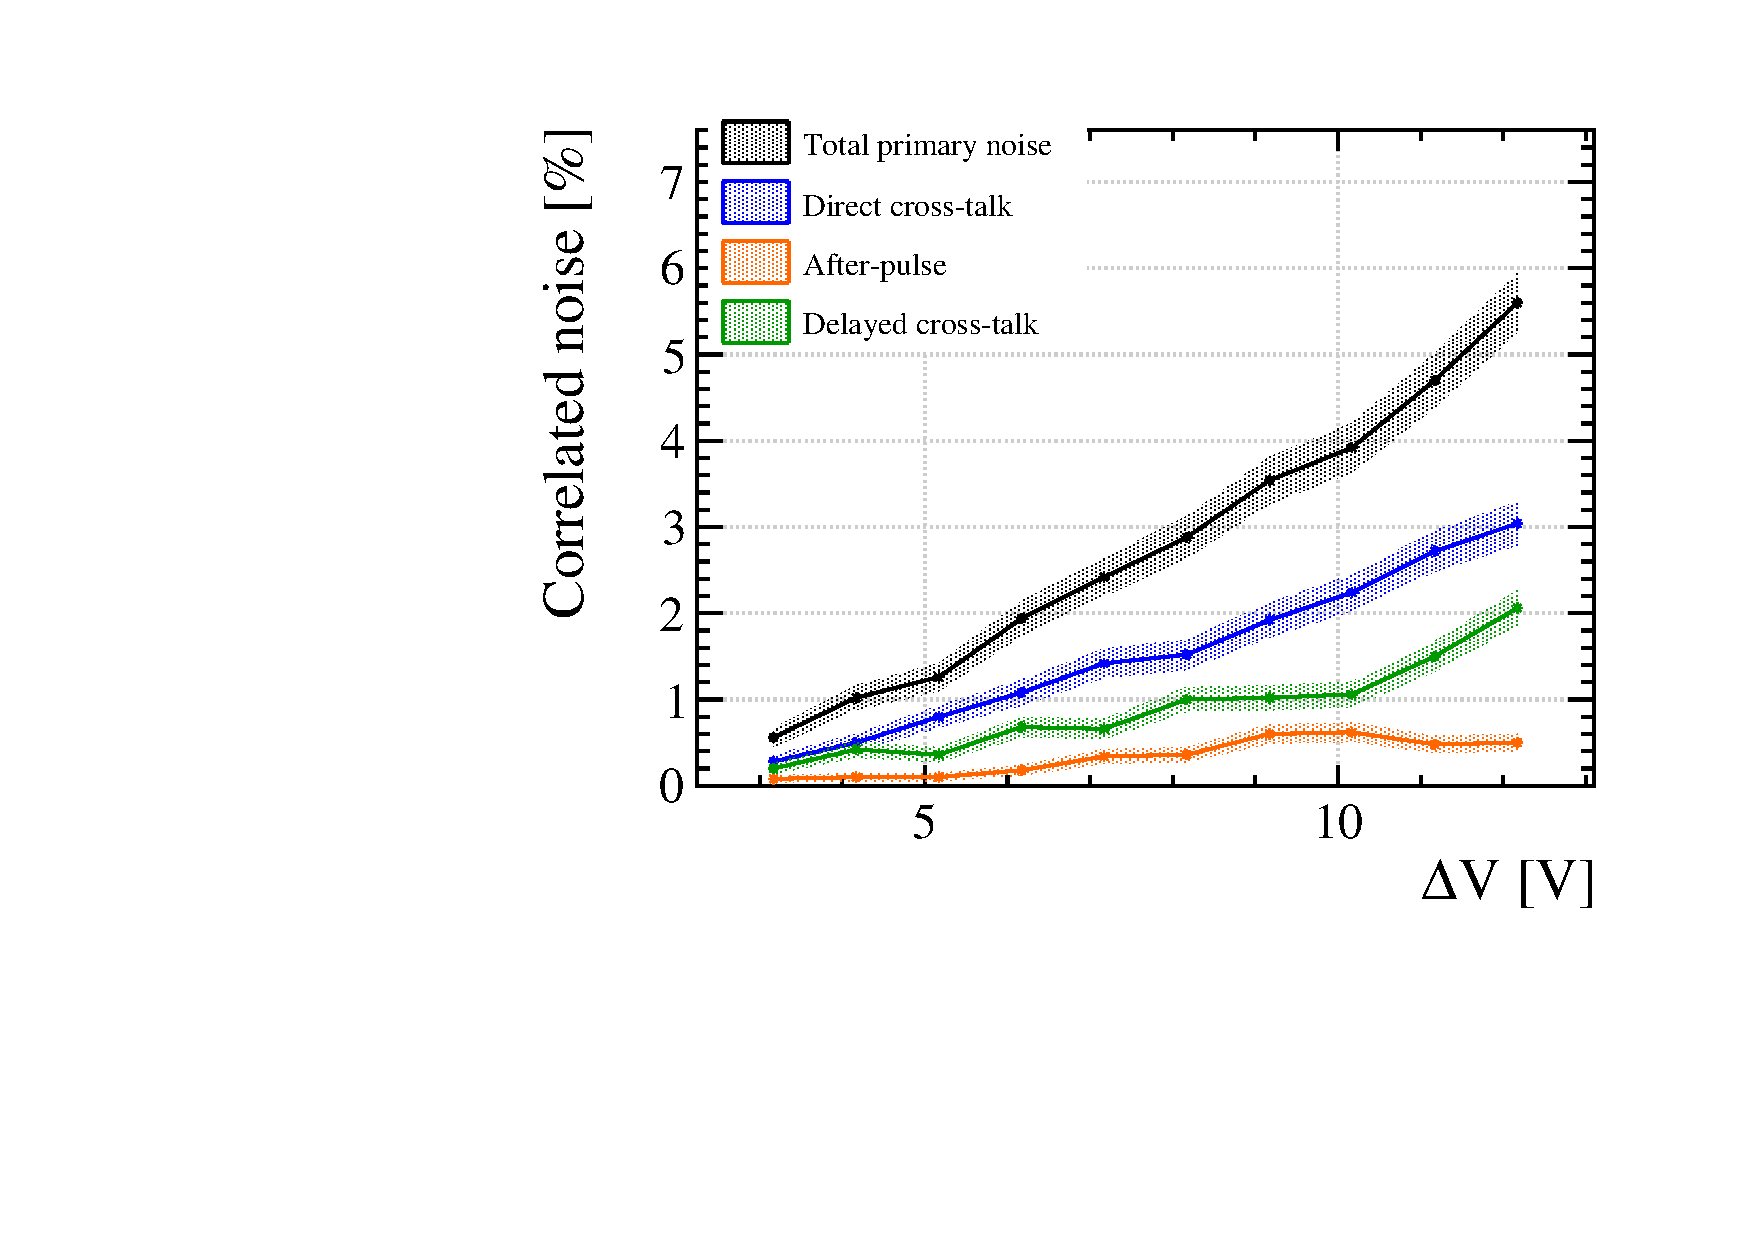
\includegraphics[width=1\linewidth]{gfx/plots/WA/31/CorrelatedNoise.pdf}
    \caption{FBK \SI{31}{\micro m}, channel $86$.}
    \label{fig:}
  \end{subfigure}
  \hfill
  \begin{subfigure}{0.48\textwidth}
    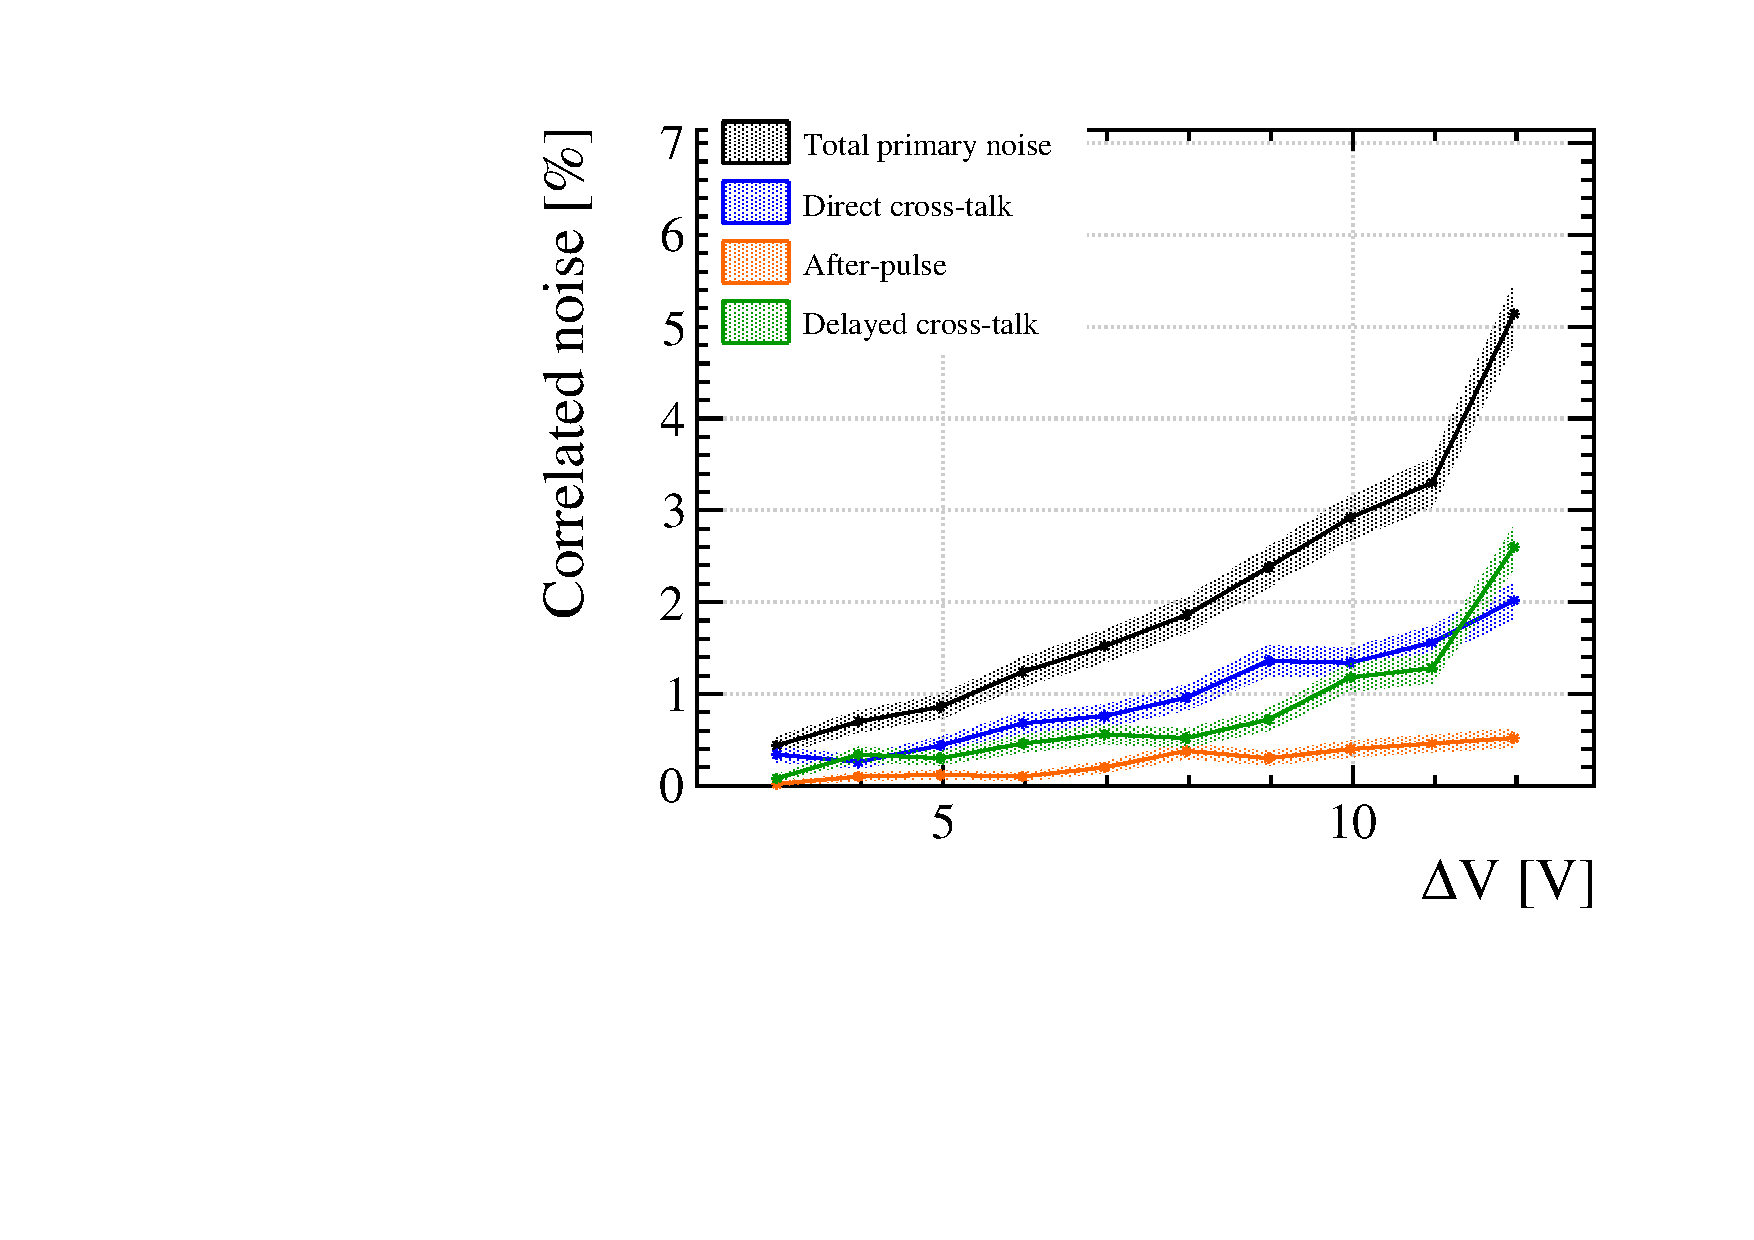
\includegraphics[width=1\linewidth]{gfx/plots/WA/42/CorrelatedNoise.pdf}
    \caption{FBK \SI{42}{\micro m}, channel $54$.}
    \label{fig:}
  \end{subfigure}
  \hfill
   \begin{subfigure}{0.48\textwidth}
    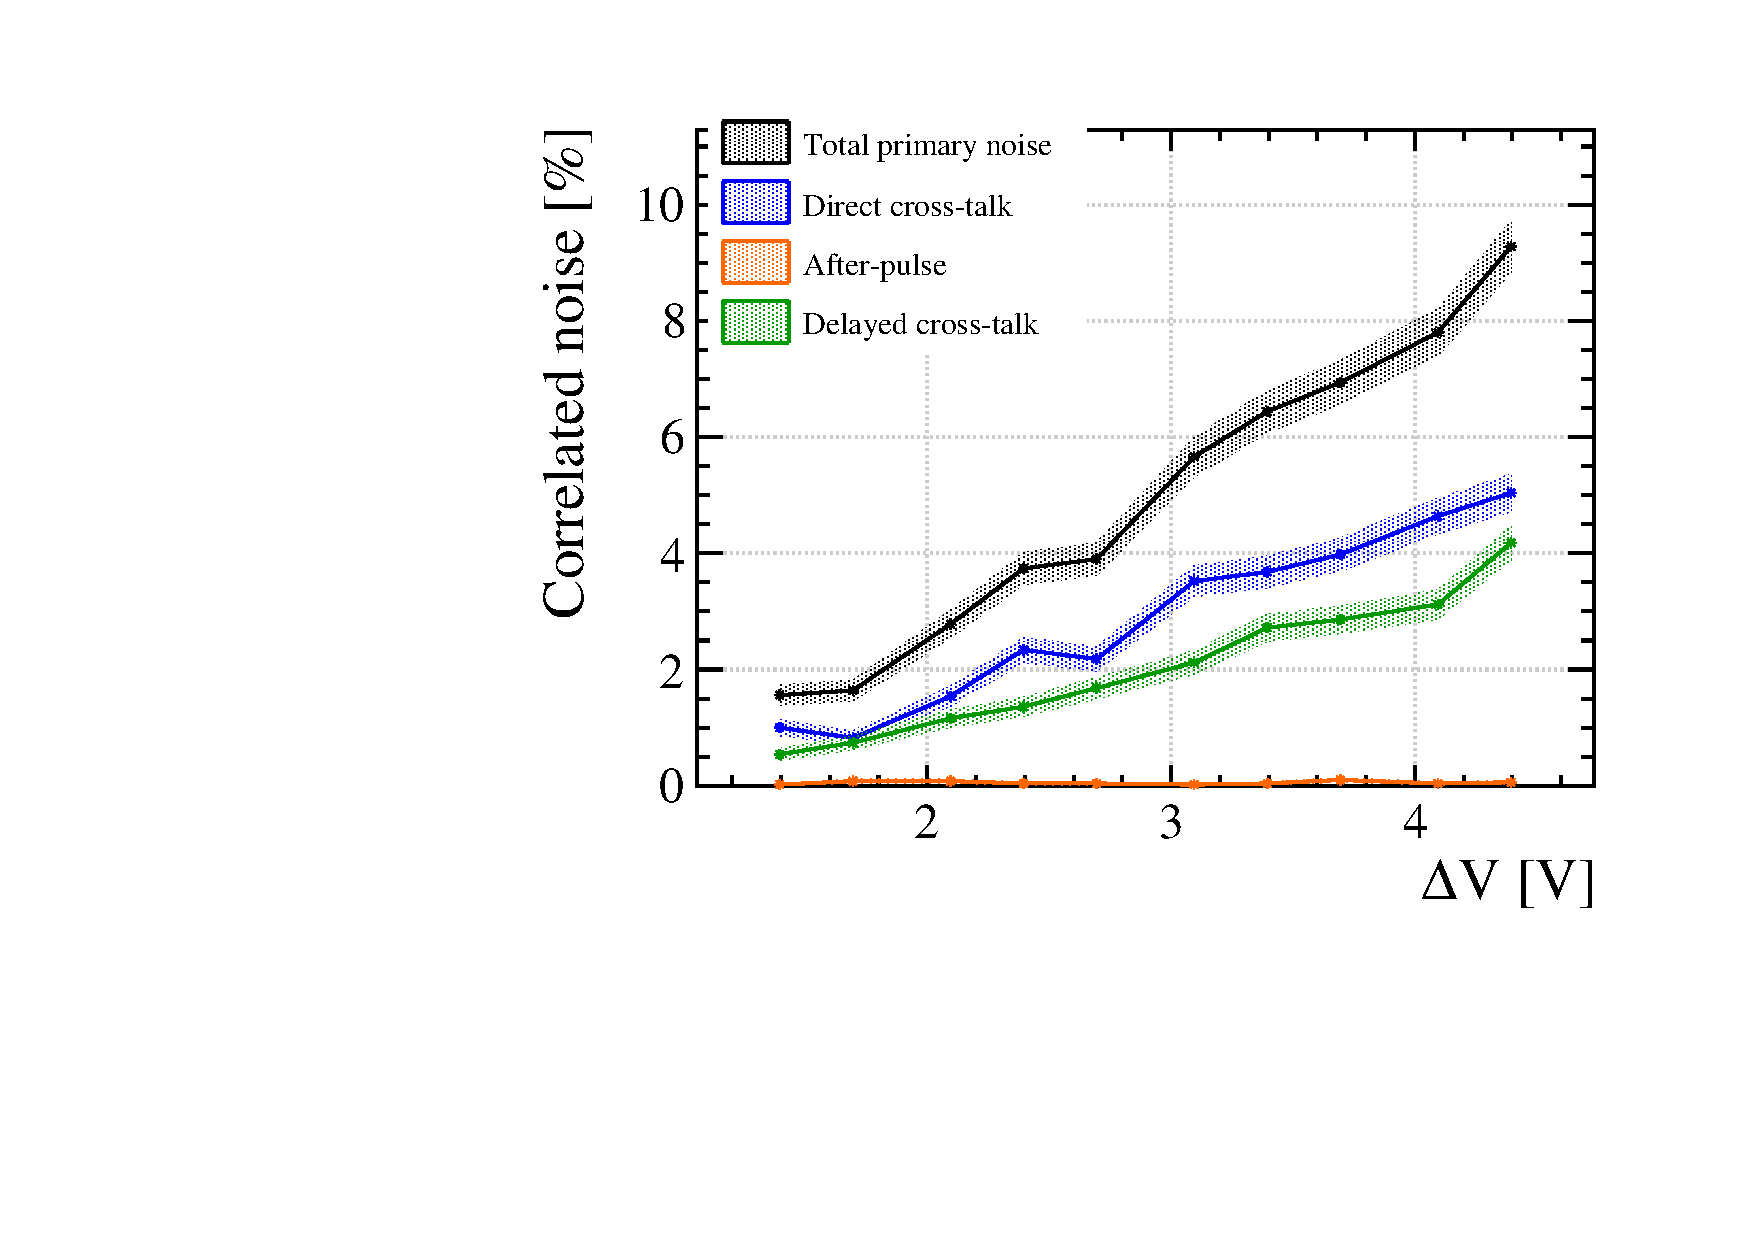
\includegraphics[width=1\linewidth]{gfx/plots/WA/H2017/CorrelatedNoise.pdf}
    \caption{H2017, channel $54$.}
  \end{subfigure}
  \hfill
   \begin{subfigure}{0.48\textwidth}
    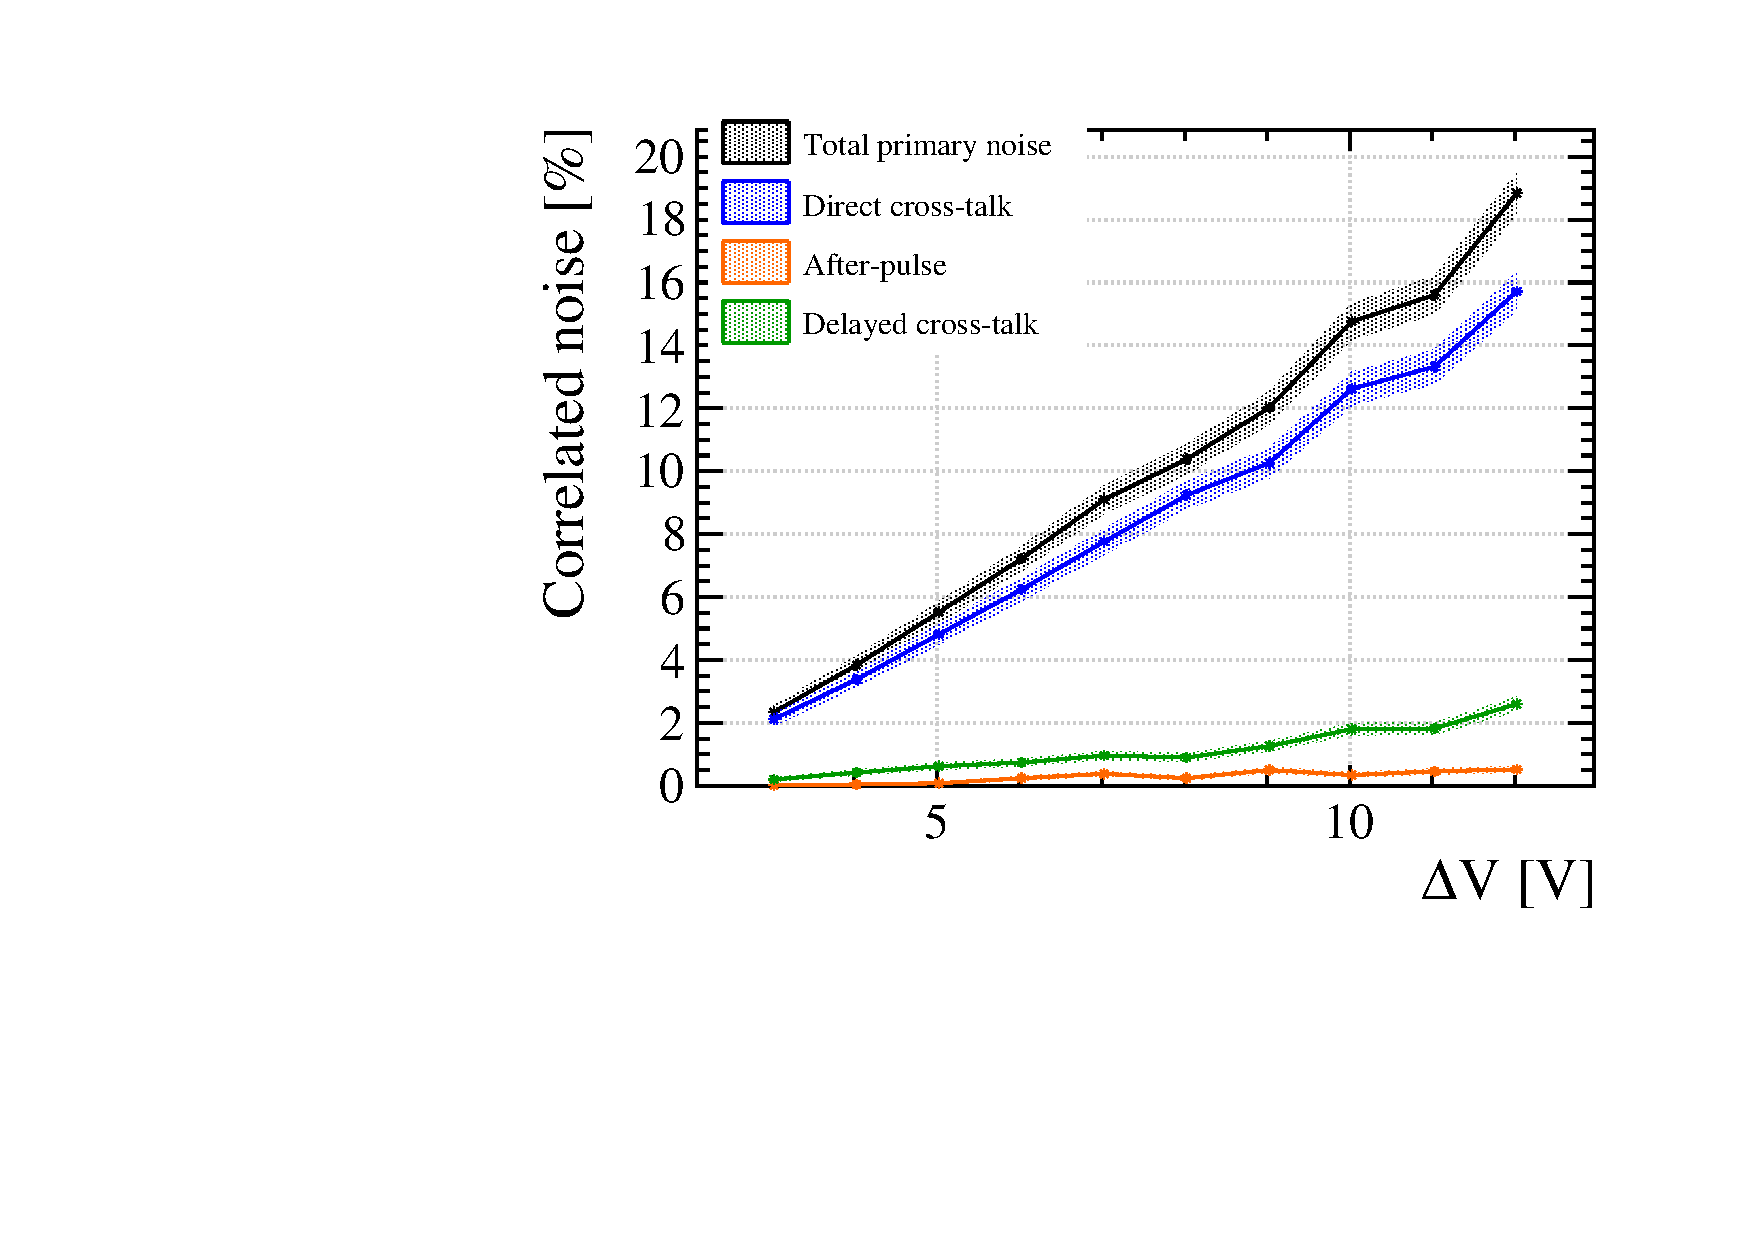
\includegraphics[width=1\linewidth]{gfx/plots/WA/31epoxy/CorrelatedNoise.pdf}
    \caption{FBK \SI{31}{\micro m} + epoxy, channel $22$.}
  \end{subfigure}
\caption{Correlated noise of the FBK \SI{16}{\micro m} (a), \SI{31}{\micro m} (b), \SI{42}{\micro m} (c), H2017 (d) and FBK \SI{31}{\micro m} + epoxy layer (e) SiPM. }
\label{fig:correlated noises + epoxy}
\end{figure}

\begin{figure}[htbp]
    \centering
       \begin{subfigure}{0.48\textwidth}
        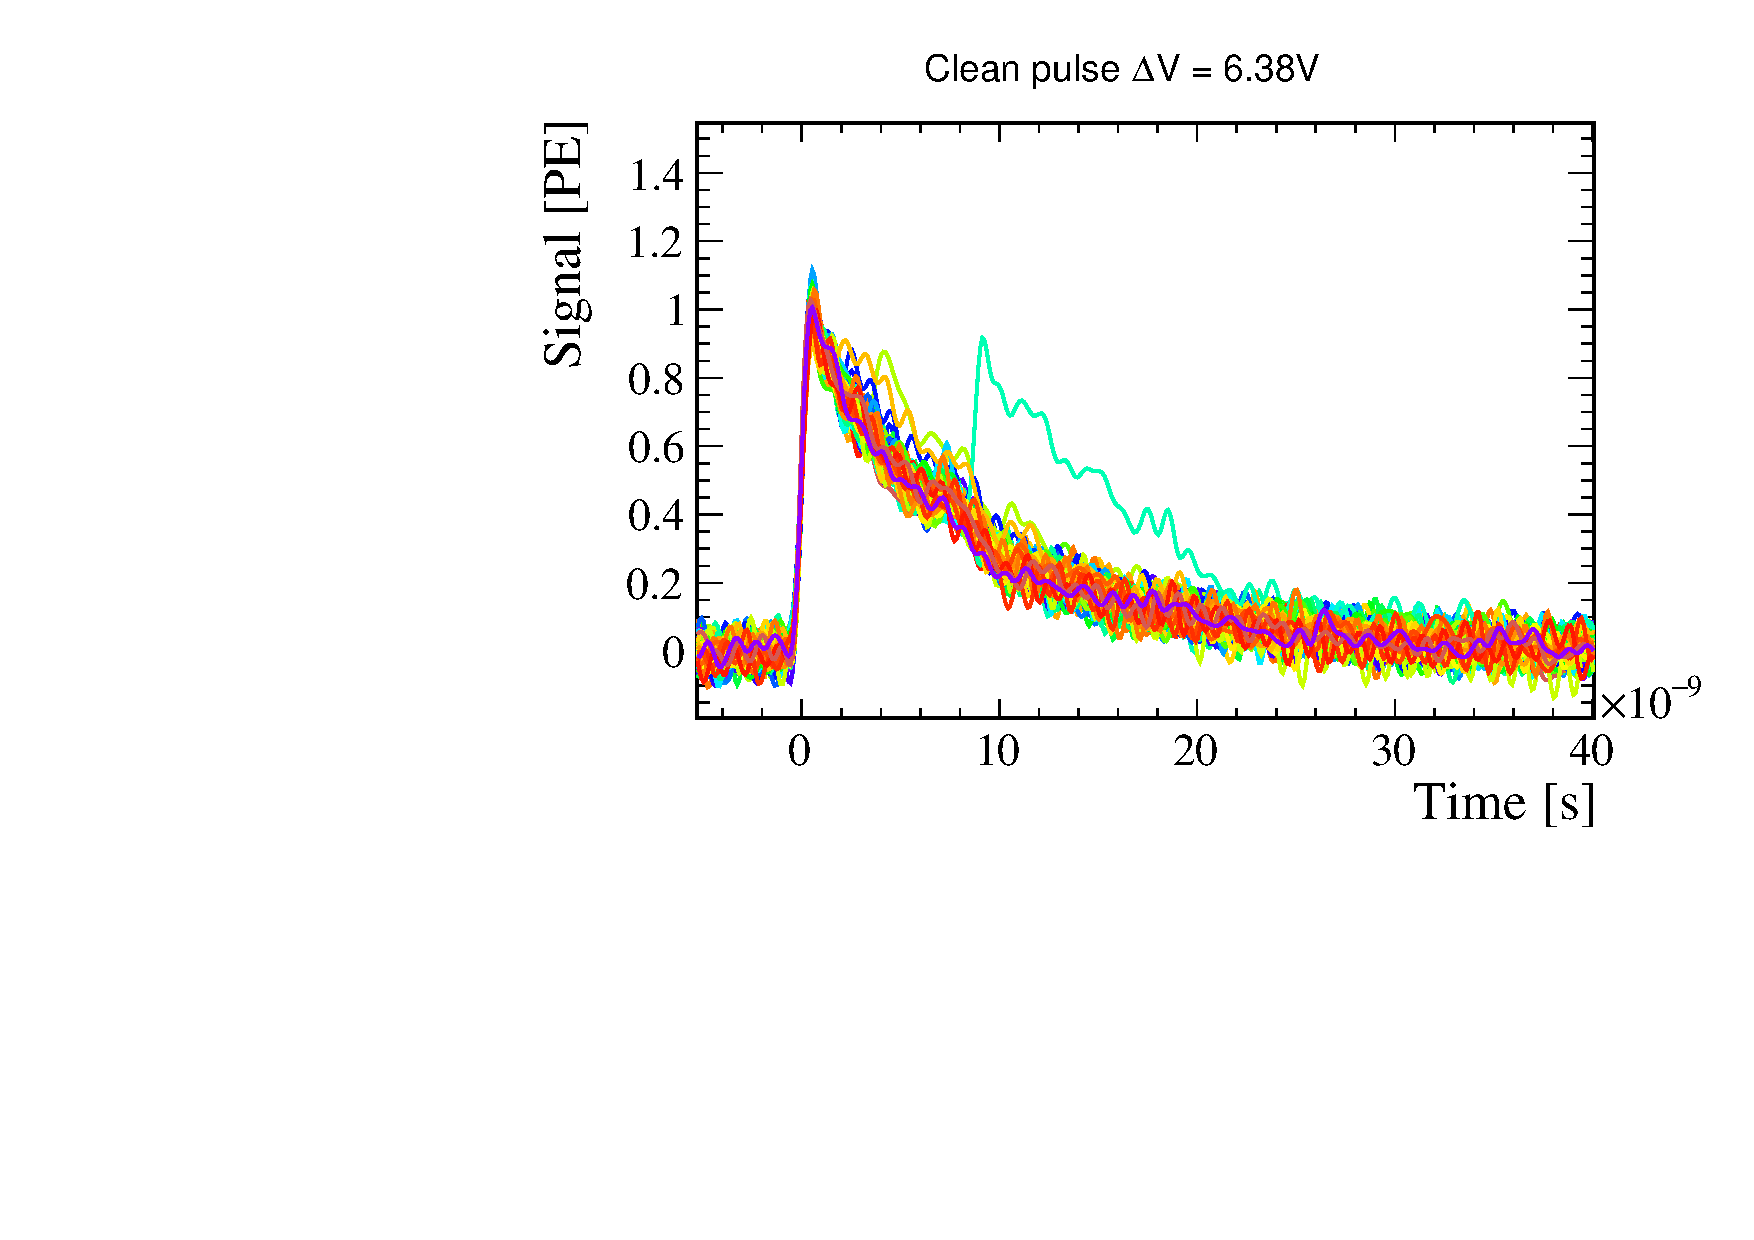
\includegraphics[width=1\linewidth]{gfx/plots/WA/16/clwf16.pdf}
        \caption{}
      \end{subfigure}
      \hfill
       \begin{subfigure}{0.48\textwidth}
        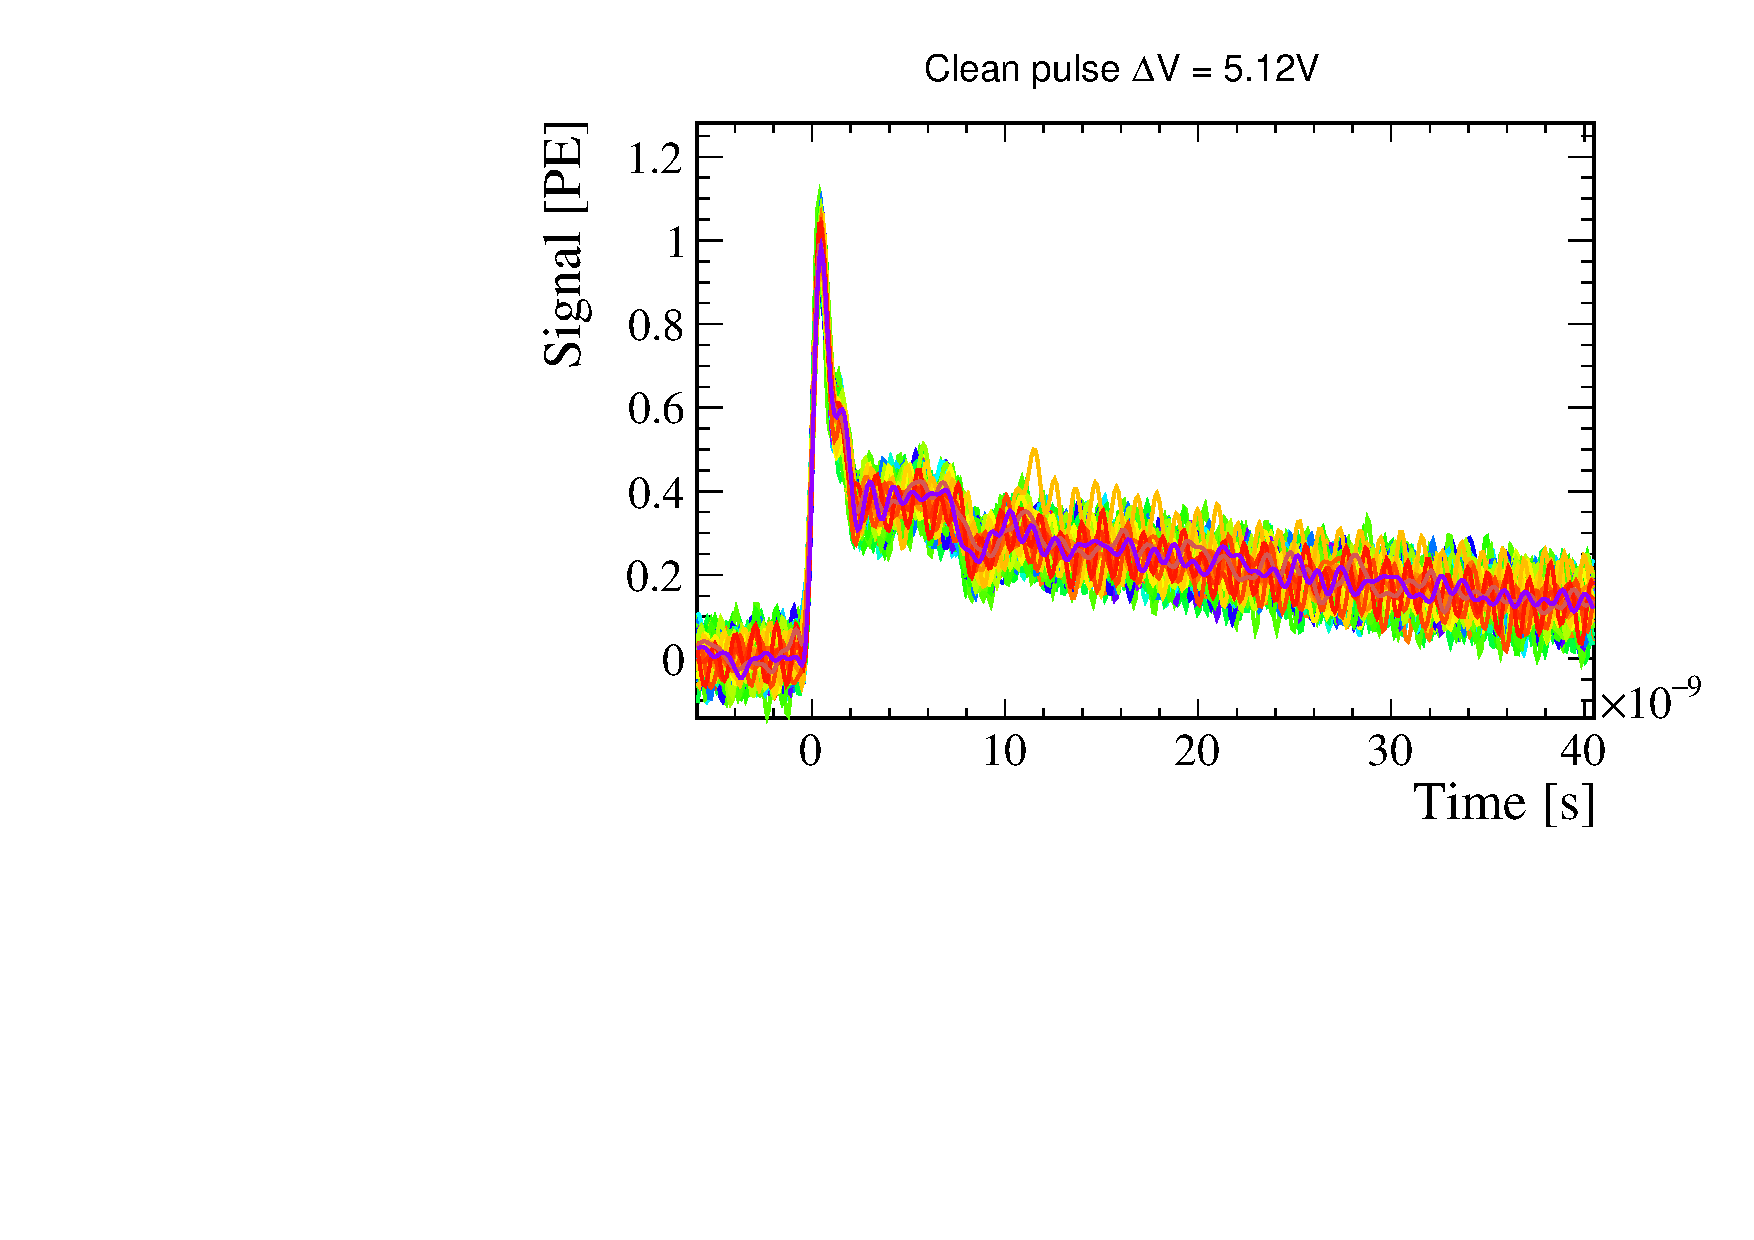
\includegraphics[width=1\linewidth]{gfx/plots/WA/31/clwf31.pdf}
        \caption{}
      \end{subfigure}
      \hfill
       \begin{subfigure}{0.48\textwidth}
        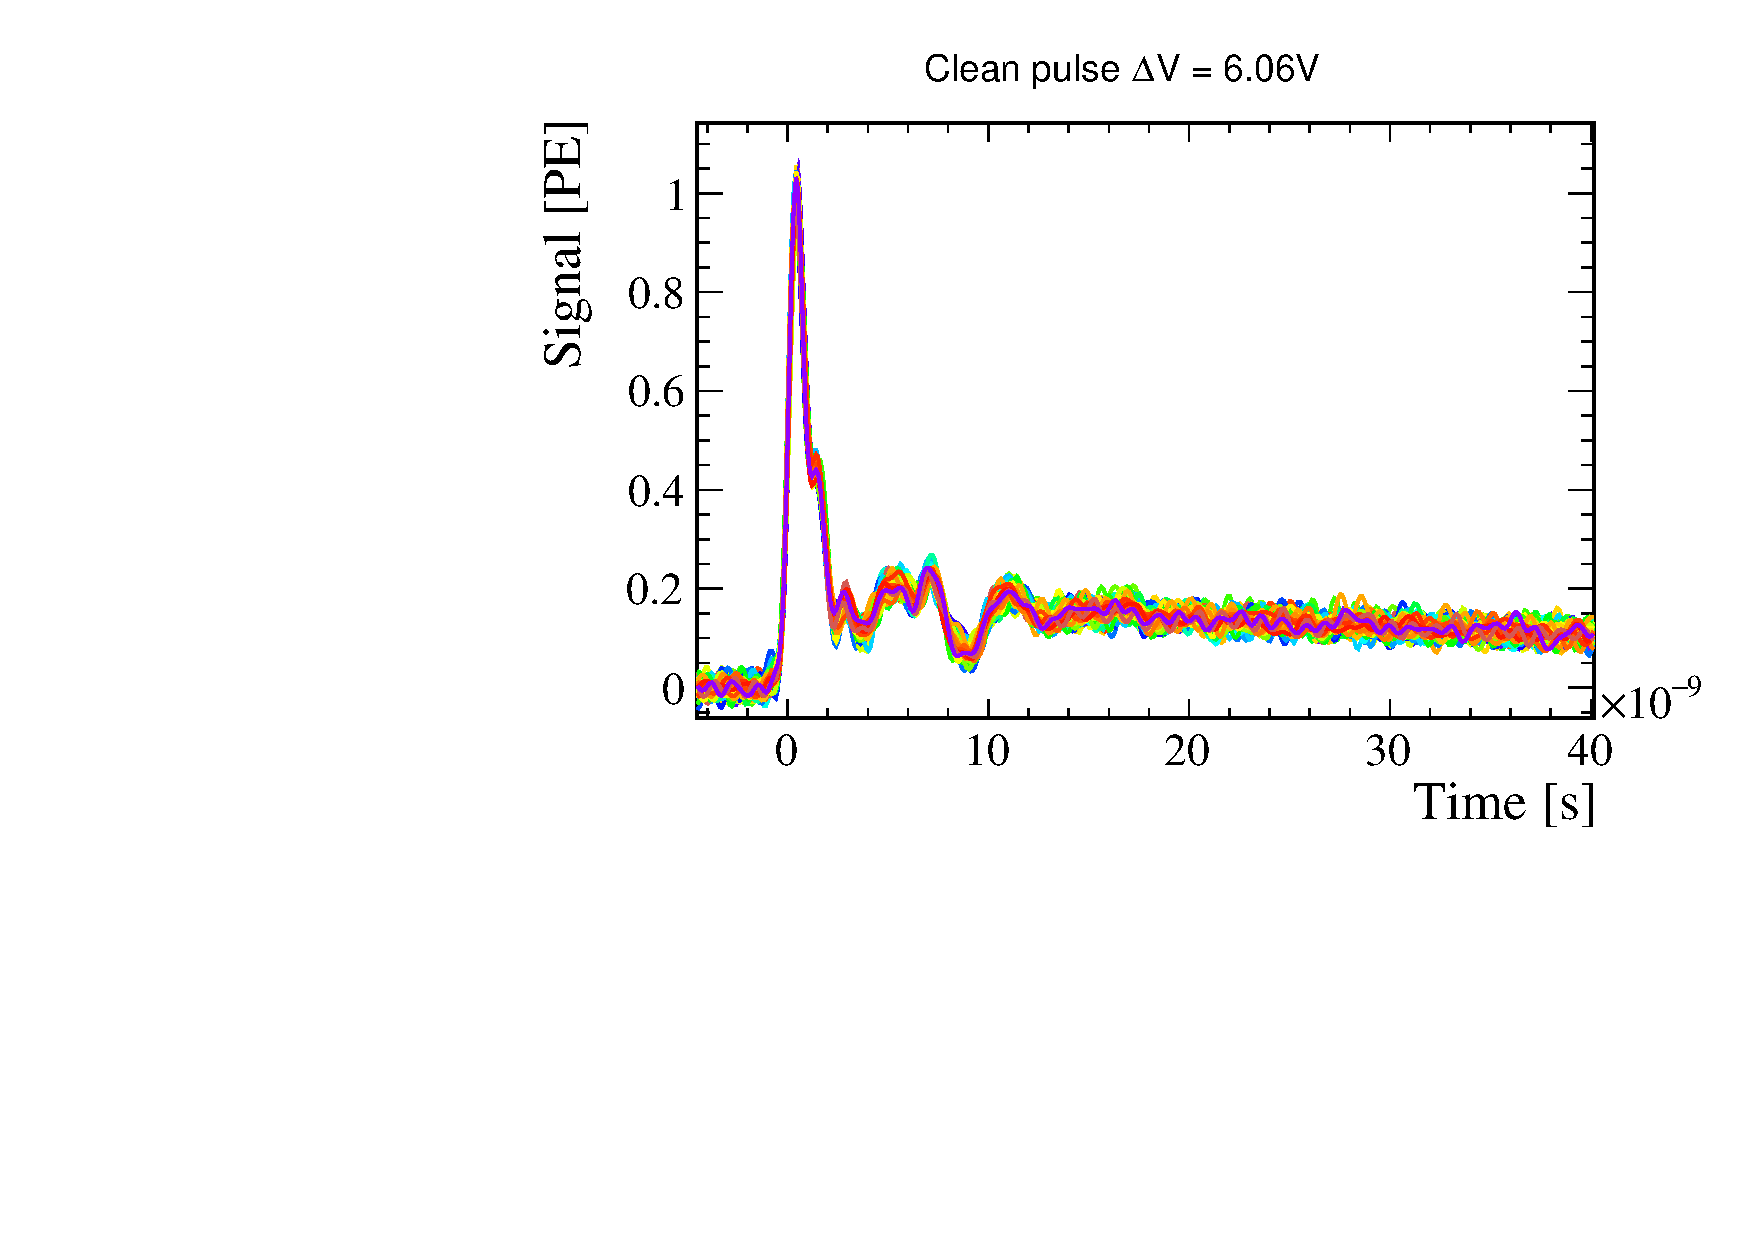
\includegraphics[width=1\linewidth]{gfx/plots/WA/42/clwf42.pdf}
        \caption{}
      \end{subfigure}
      \hfill
       \begin{subfigure}{0.48\textwidth}
        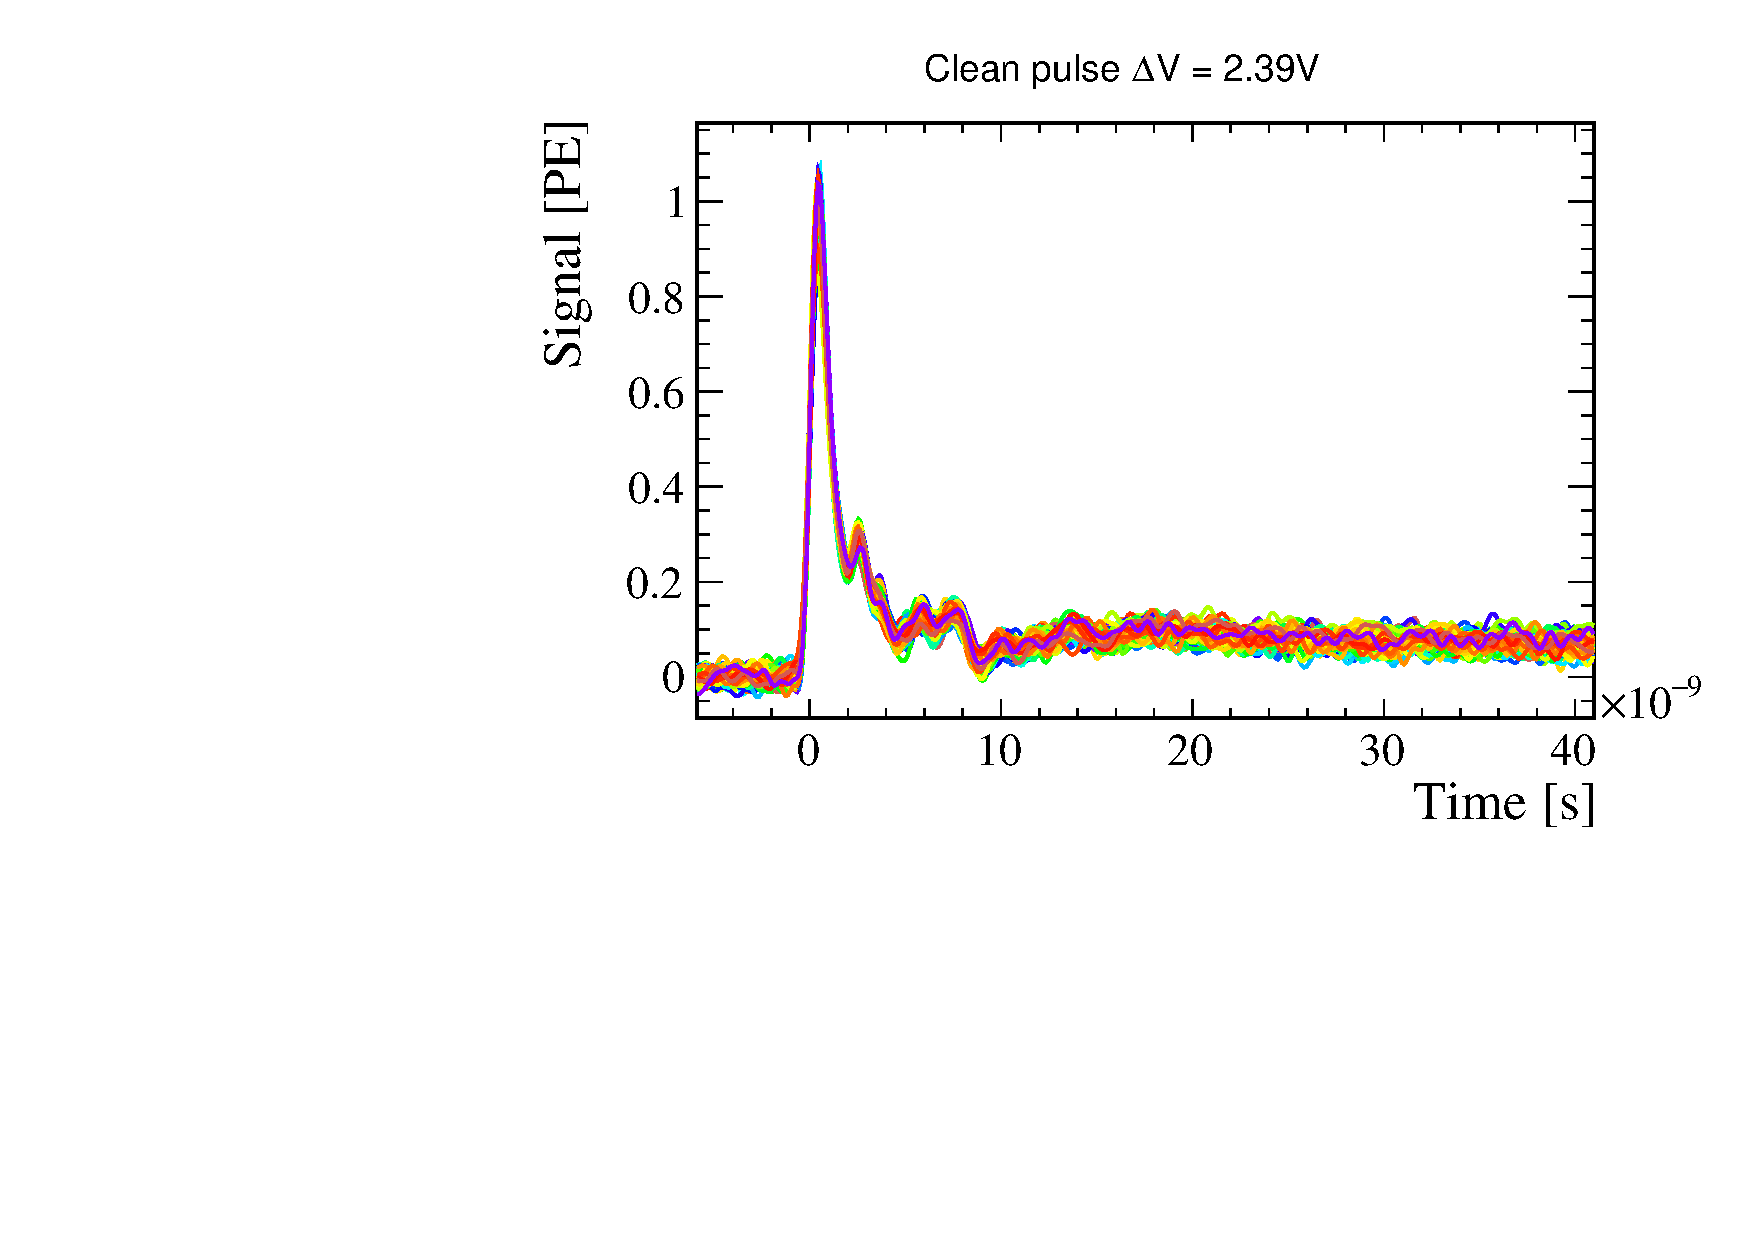
\includegraphics[width=1\linewidth]{gfx/plots/WA/H2017/clwfh2017.pdf}
        \caption{}
      \end{subfigure}
    \caption{Clean waveforms for the FBK \SI{16}{\micro m} (a), \SI{31}{\micro m} (b), \SI{42}{\micro m} (c) and Hamamatsu H2017 (d).}
    \label{fig:pulse shape clean waveforms}
\end{figure}

\restoregeometry

\begin{figure}[htbp]
    \centering
    \begin{subfigure}{0.7\textwidth}
        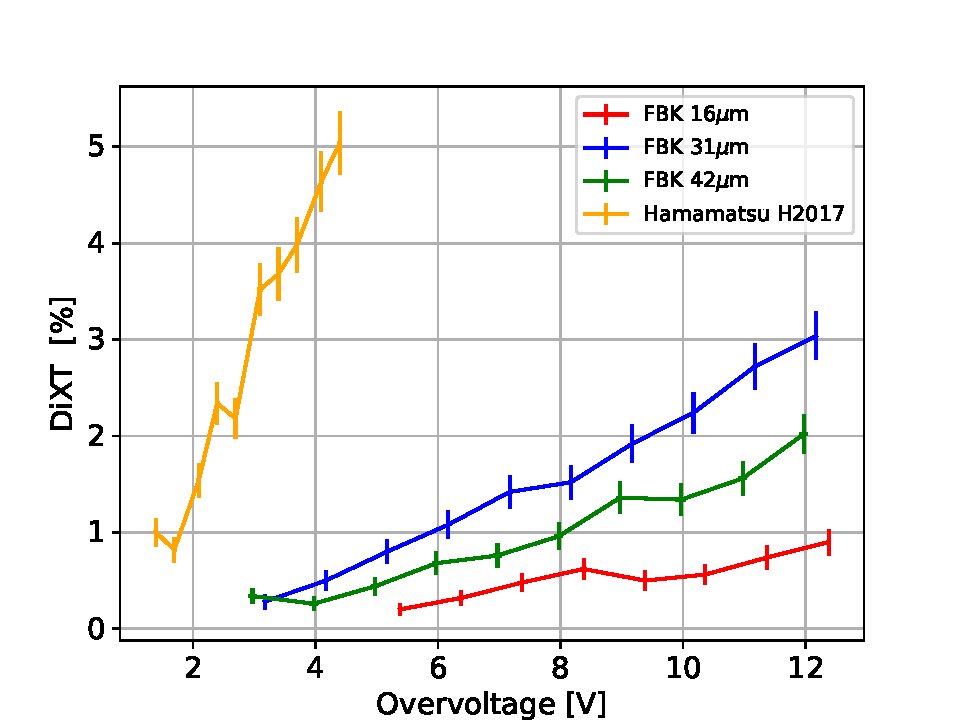
\includegraphics[width=\textwidth]{gfx/plots/WA/DiXTs_wo_epoxy.pdf}
        \caption{}
    \end{subfigure}
    \hfill
    \begin{subfigure}{0.7\textwidth}
        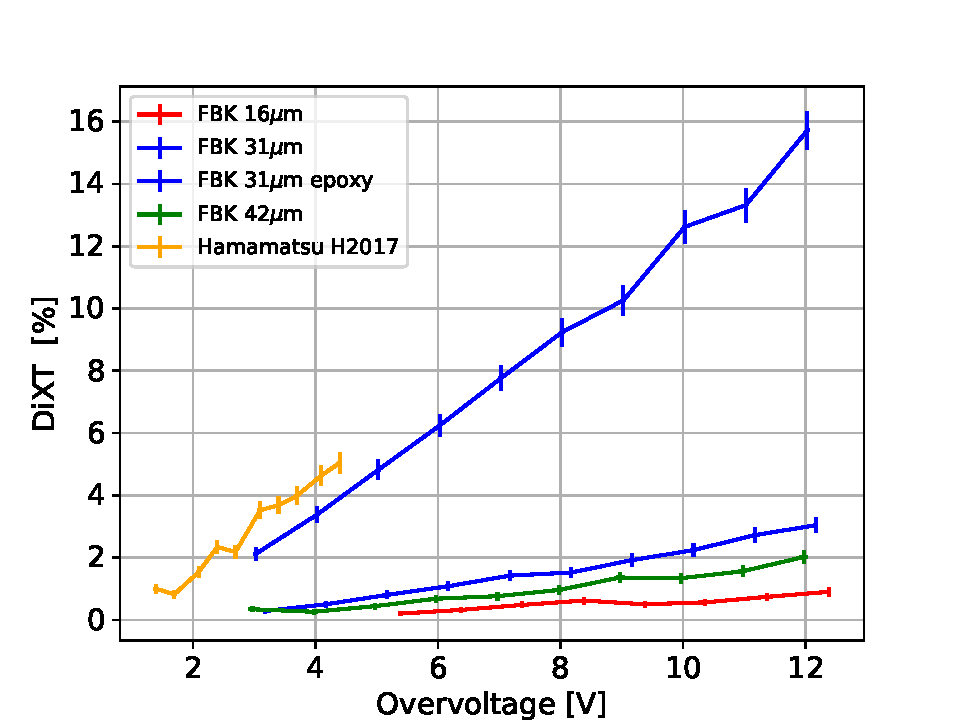
\includegraphics[width=\textwidth]{gfx/plots/WA/DiXTs.pdf}
        \caption{}
    \end{subfigure} 
    \caption{DiXT for the different four studied detectors (a) and with the \SI{31}{\micro m} with the epoxy layer (b).}
    \label{fig:DiXT detectors}
\end{figure}


% fbk and hamamatsu
The first observation one can make about the FBK detectors is their very low correlated noise even at high overvoltage. At $\Delta V= 12$ V, the FBK have $4\%$ to $6\%$ of total correlated noise. The Hamamatsu cannot operate in this region, but at its maximal operation range (around $\Delta V= 5$ V), the Hamamatsu is at $\approx 9.5\%$ of total correlated noise. At this $\Delta V$ the FBK detectors have $8$ to $12$ times less correlated noise. Having a higher operation range without increasing the correlated noise helps in improving the PDE. This difference is highlighted by Fig. \ref{fig:DiXT detectors} (a) where the DiXT is very low the for the FBK detectors. Operating at high PDE reduces the errors on $V_{bd}$ since we work in wider operation range. 
\\
The FBK \SI{16}{\micro m} has more DeXT than DiXT, which is not the case for the two other detectors from FBK. This may be due to a misidentification between direct and delayed cross talk. The pulse shapes for the four detectors are very different, and shown in Fig. \ref{fig:pulse shape clean waveforms}. One can see on the \SI{16}{\micro m} (a) that one signal is misidentified as 'clean' (in pale blue). Also, since the pixel sizes are smaller for the \SI{16}{\micro m} and \SI{31}{\micro m}, the signal amplitude is also smaller resulting in a lower signal to noise ratio. It is clearly visible on Fig. \ref{fig:pulse shape clean waveforms} (a) \& (b) where the baseline is way thicker than for the bigger pixel sizes (c) \& (d).\\ 
%31um epoxy talk 
\\
An interesting comparison between the FBK \SI{31}{\micro m} and its version with the epoxy layer can be done. Correlated noise plots are shown in Fig. \ref{fig:correlated noises + epoxy} (b) \& (e) respectively. The addition of an epoxy layer increases the total correlated noise by a factor of $6$ for all the overvoltage range. This result is explained by the fact that most of the noise comes from external cross talk. The photons issued from an avalanche by bremsstrahlung may be reflected by the epoxy layer, allowing this photon to hit another neighbour pixel causing external cross talk. Delayed cross talk is also increased.

%\begin{table}[]
%\begin{tabular}{|c|c|c|c|c|}
%\hline
%Detector                            & FBK \SI{16}{\micro m}   & FBK \SI{31}{\micro m} & FBK \SI{42}{\micro m} & H2017         \\ \hline
%Operation range$\cdot \Delta V$ [V] & [$5.4$-$12.4$] & [$3$-$12$]   & [$3$-$12$]   & [$0.8$-$4.6$] \\ \hline
%\end{tabular}
%\caption{Operation range for the studied detectors.}
%\label{table:operation ranges}
%\end{table}

\section{Gain}
\label{ch:Results:Gain}


The gain results are shown in Fig. \ref{fig:Gain fit for all detectors} and presented per unit of overvoltage.

Difficulties in the measurements have been encountered especially at low operation voltages for the FBK detectors. As explained in section \ref{ch:Results:Noise Classification}, the noise is very present at low $\Delta V$ for small pixel size (smaller pulse amplitude). 

\begin{figure}[htbp]
    \centering
    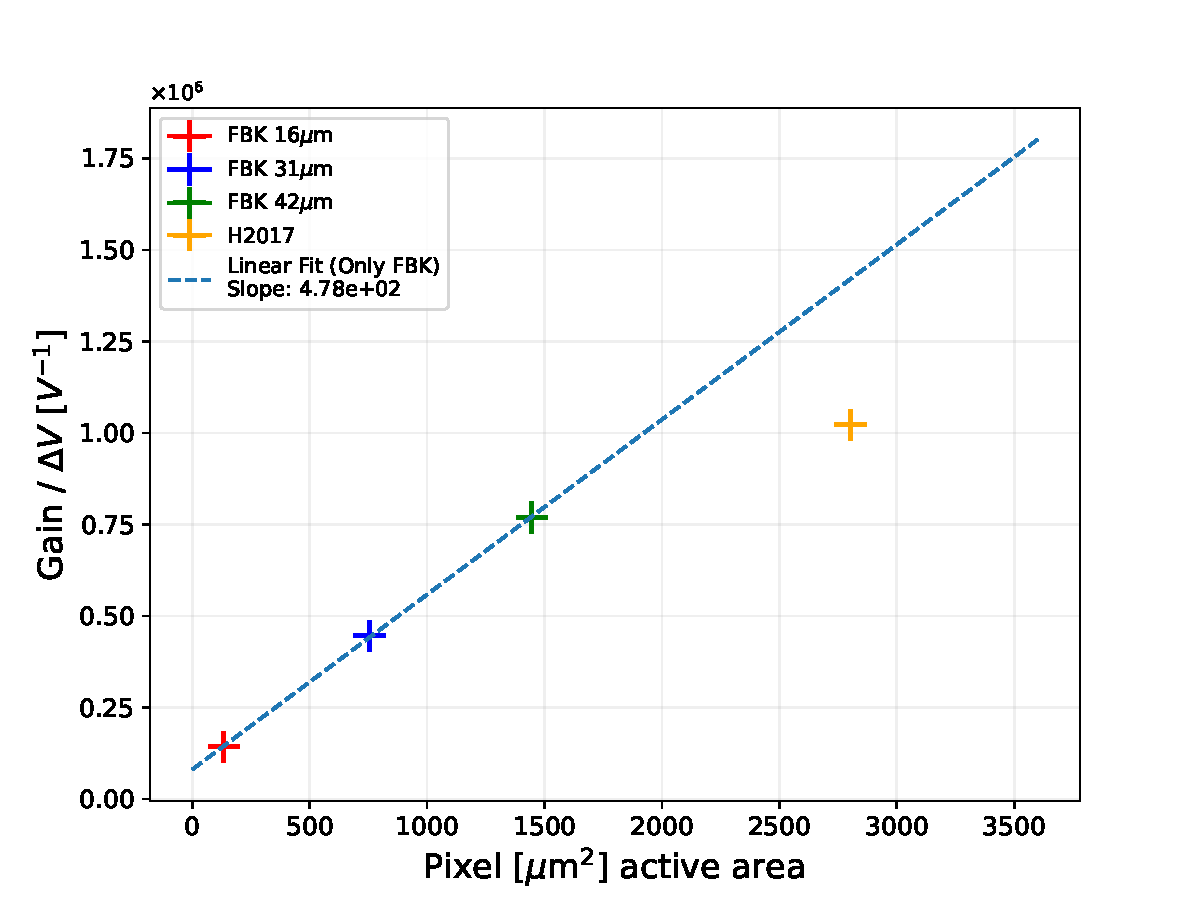
\includegraphics[width=0.8\textwidth]{gfx/plots/Gain/Gain(pixel size)_area.pdf}
    \caption{Relation between the gain and the pixel active area.}
    \label{fig:gain(area)}
\end{figure}


The first observation is that the measured value for the Hamamatsu H2017 matches with \cite{Girard2018CharacterisationDistributions}. 
\\
The smaller the pixel size, the smaller the gain. This is confirmed by the measurement where the FBK \SI{16}{\micro m} has the smallest gain value, followed by the \SI{31}{\micro m} and then \SI{42}{\micro m}. The reason why the gain depends on the pixel size is purely physical; the more active area (hence pixel size), the more electron-hole pair will be created during the avalanche and hence more current is produced. 
An interesting comparison is shown in Fig. \ref{fig:gain(area)}. Here, the gain as a function of the active area. Ideally, it would be a good choice to represent the gain as a function of the total active volume, but the thickness of the layers is not known. The surface plot is still valid at first approximation since the 3 samples from FBK analyzed are from the same wafer (W1). The thickness of the sample vary only due to some disparities but the process of adding the thin layers is considered homogeneous. A linear relation is clearly visible on Fig. \ref{fig:gain(area)} and confirms the gain dependency to the active volume. The Hamamatsu is shown as comparison and of course do not have the same dependency since it is not the same technology, wafer and process of fabrication. \\
\\
These gain measurements also provide inputs on the $V_{bd}$, the $V_{offset}$ represents the difference between $V_{bd,WA}$ from the waveform analysis and $V_{bd,G}$ by quantifying this difference at the extrapolation to zero of the fit. Significant differences from \SI{-0.8}{\volt} to \SI{+0.3}{\volt} showed that the $V_{WA,bd}$ may not be accurate enough especially for the H2017 where the gain is well fitted. Nevertheless, the gain measurement of the FBK are less precise, and we will see later \ref{ch:Results:PDE} that is has less influence on the PDE. 

\newgeometry{left=0.8cm,right=0.8cm,top=2cm,bottom=2cm}

\begin{figure}[htbp]
  \centering
  \begin{subfigure}{0.48\textwidth}
    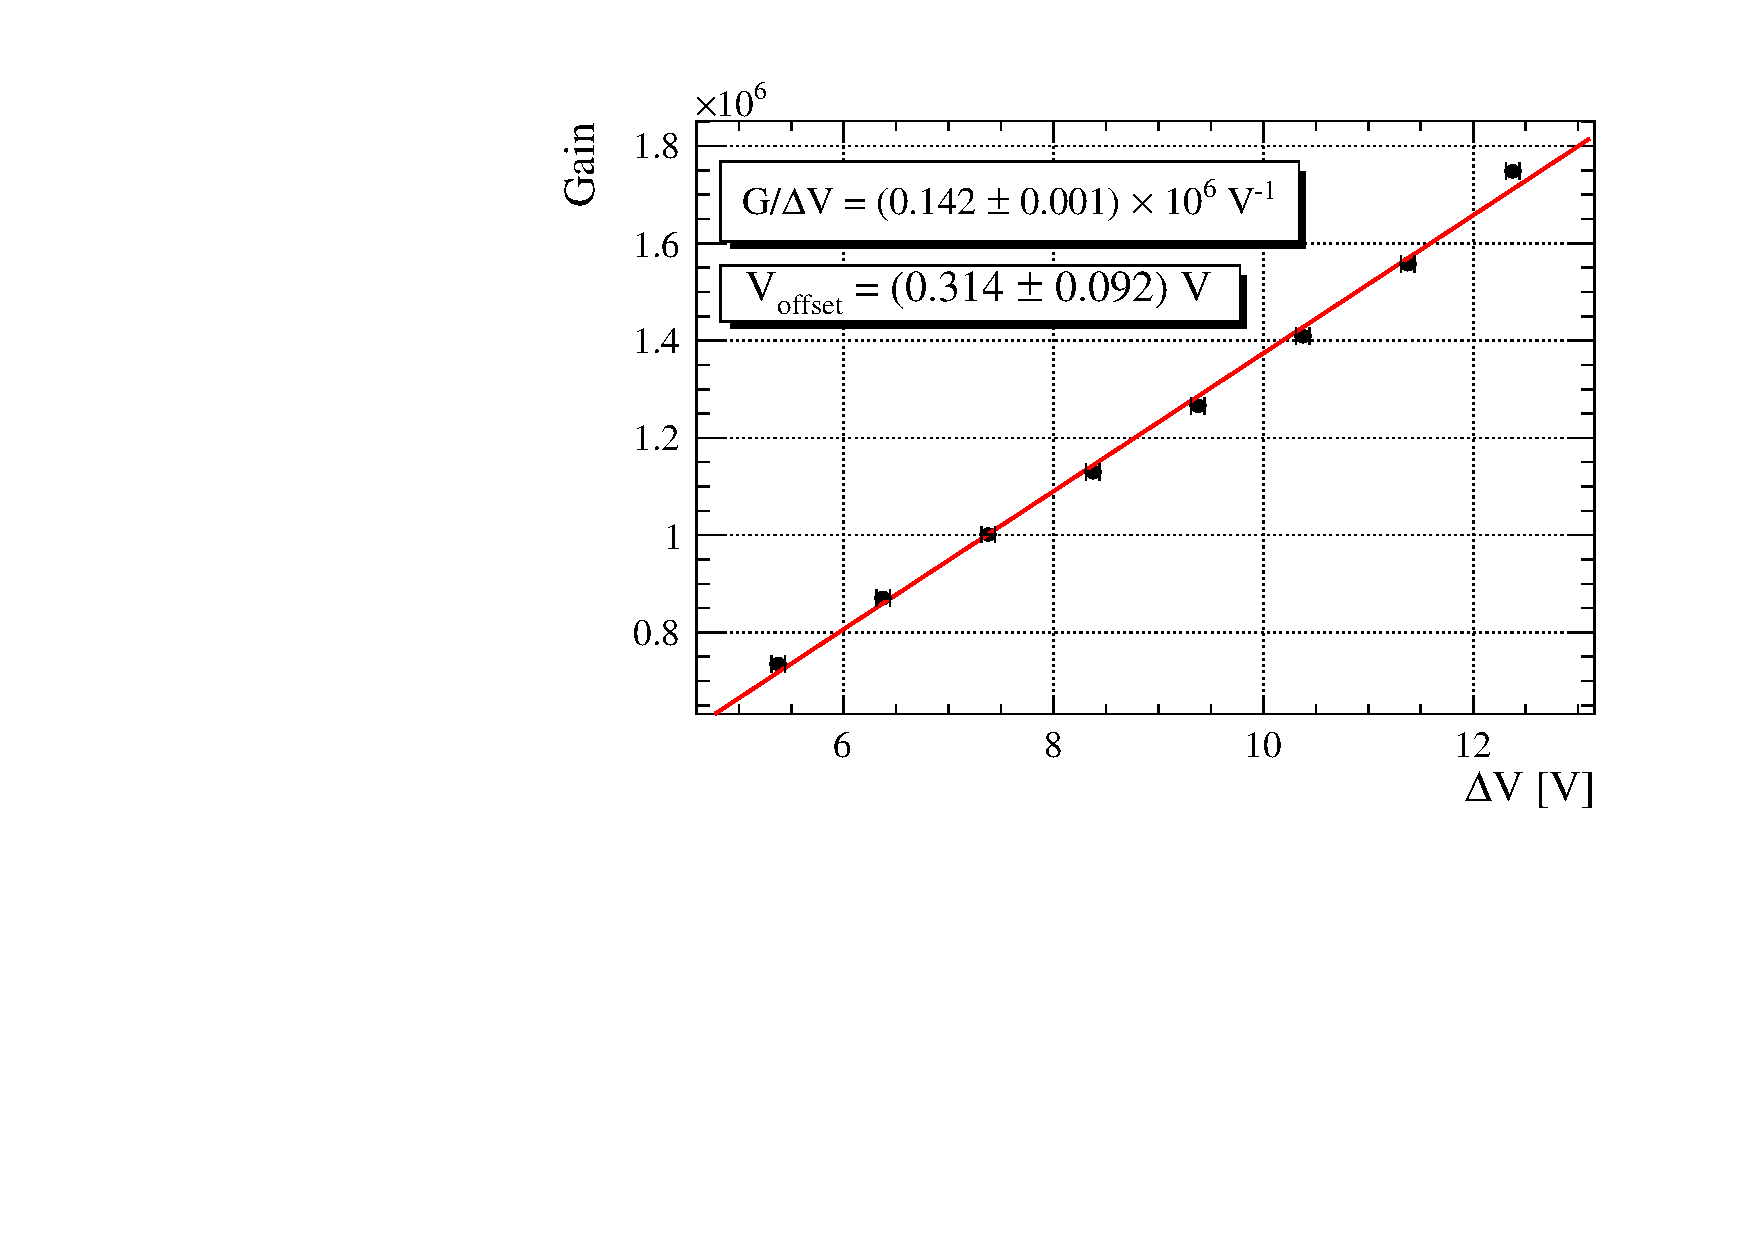
\includegraphics[width=\textwidth]{gfx/plots/Gain/16/Gain.pdf}
    \caption{FBK \SI{16}{\micro m}, channel $70$.}
    \label{fig:16 gain}
  \end{subfigure}
  \hfill
  \begin{subfigure}{0.48\textwidth}
    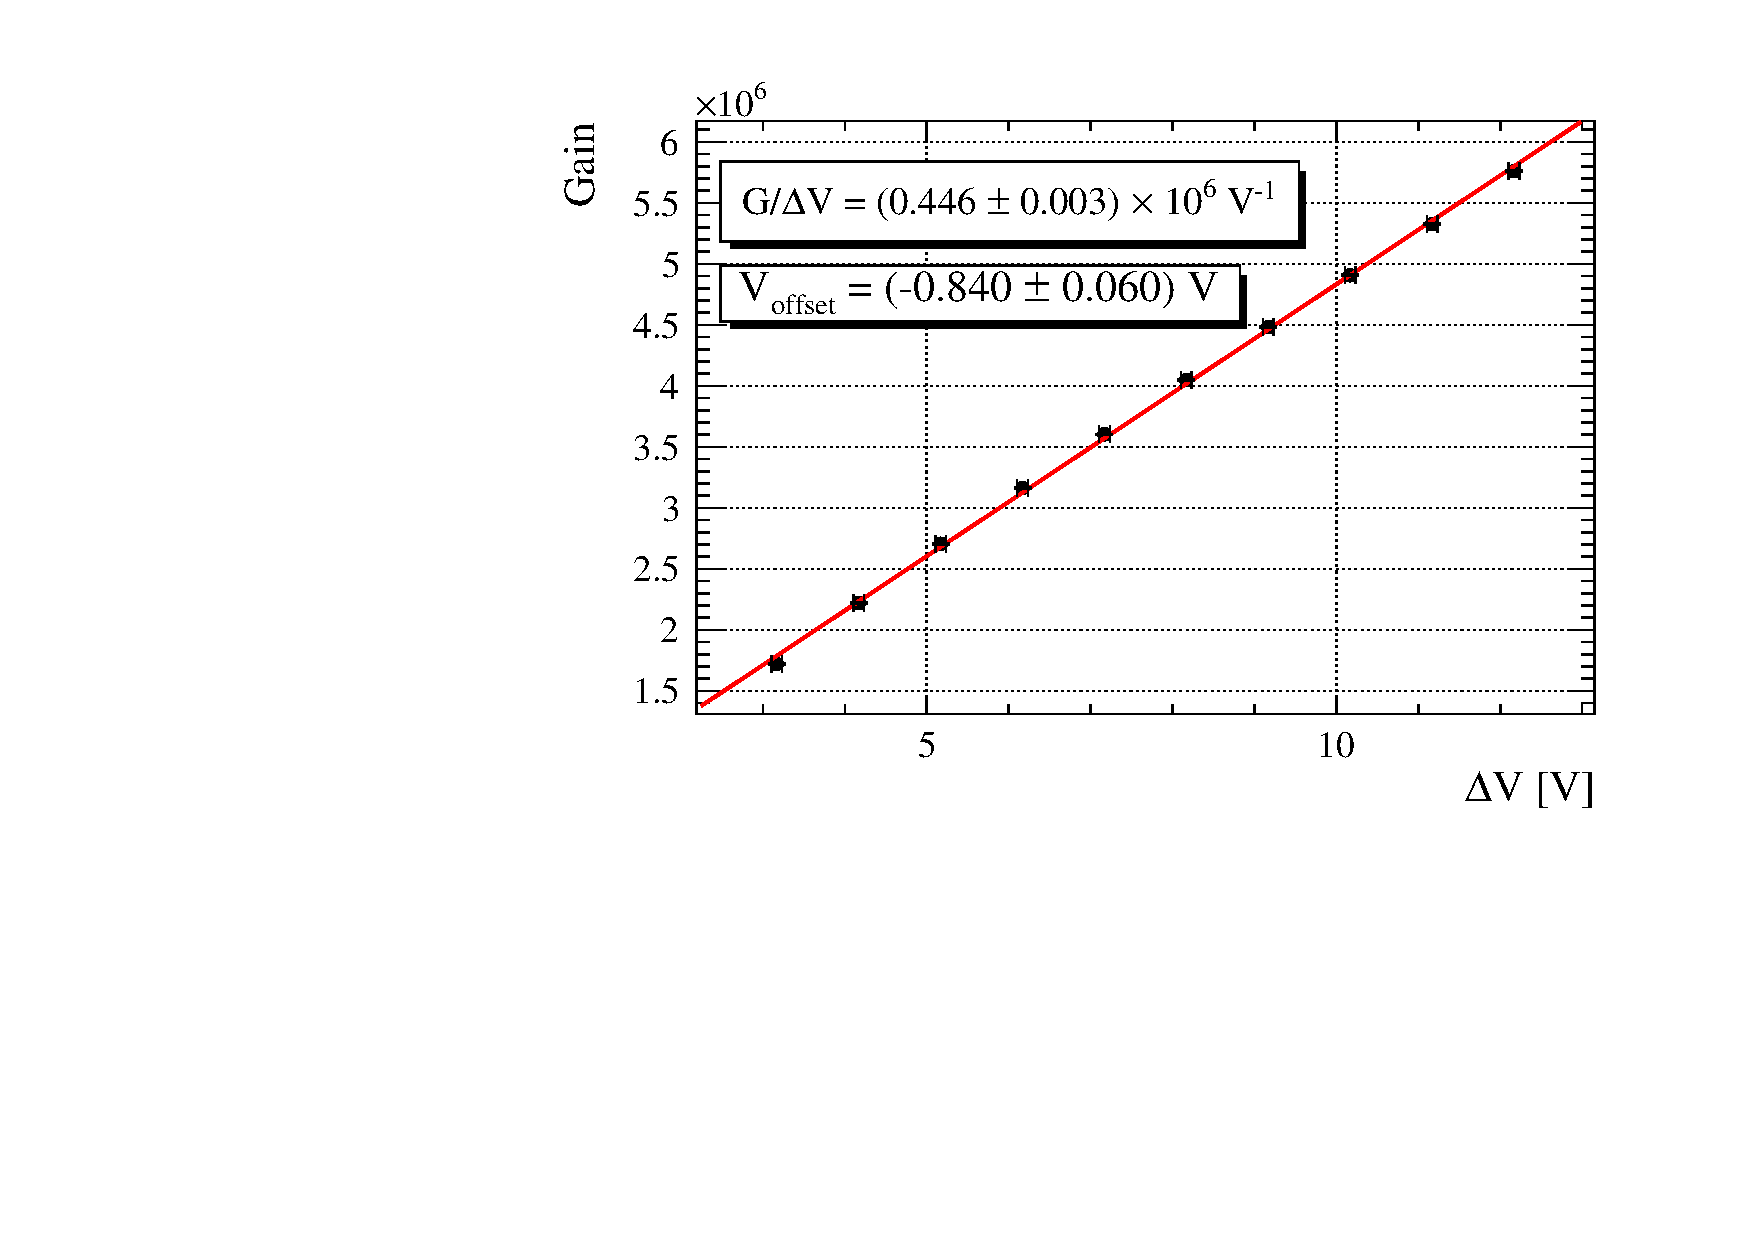
\includegraphics[width=\textwidth]{gfx/plots/Gain/31/Gain.pdf}
    \caption{FBK \SI{31}{\micro m}, channel $86$.}
    \label{fig:31 gain}
  \end{subfigure}
    \begin{subfigure}{0.48\textwidth}
    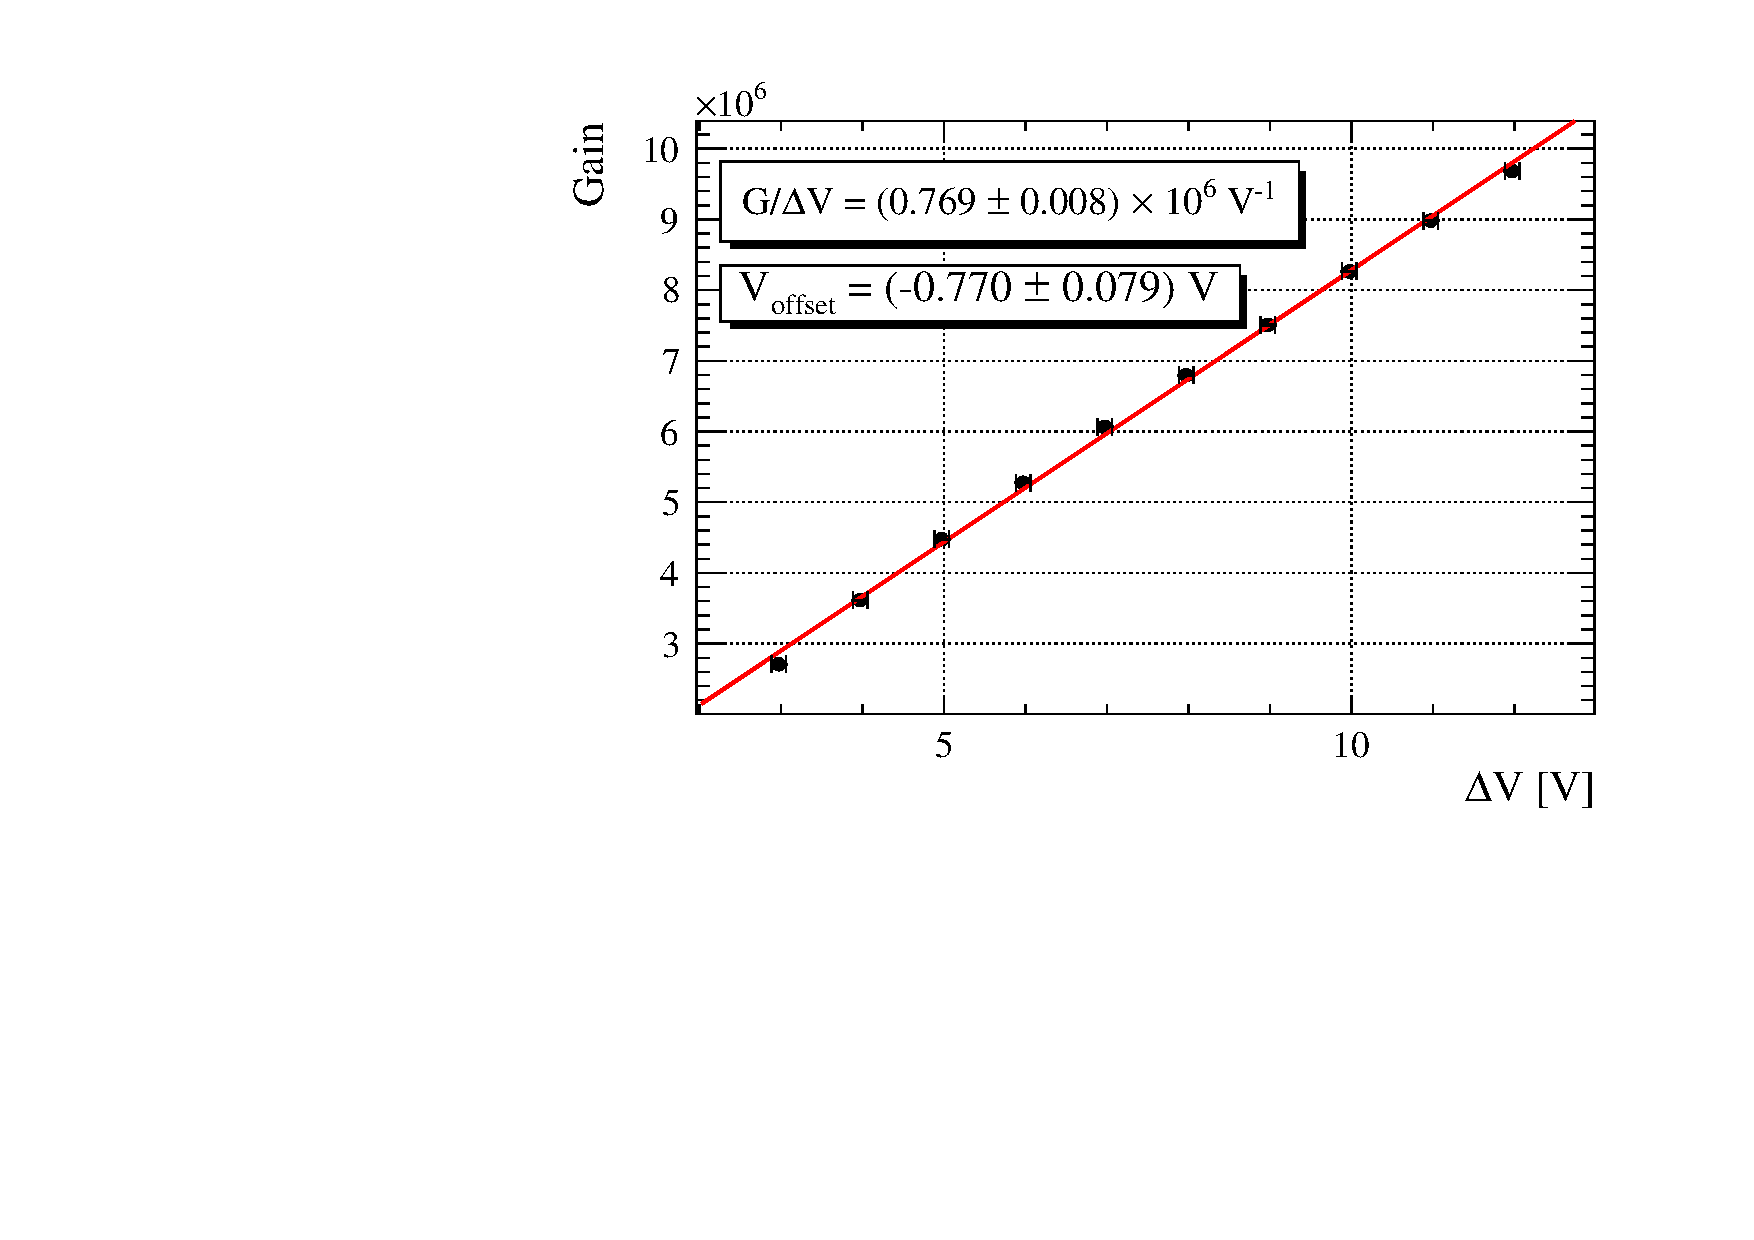
\includegraphics[width=\textwidth]{gfx/plots/Gain/42/Gain.pdf}
    \caption{FBK \SI{42}{\micro m}, channel $22$.}
    \label{fig:42 gain }
  \end{subfigure}
  \hfill
  \begin{subfigure}{0.48\textwidth}
    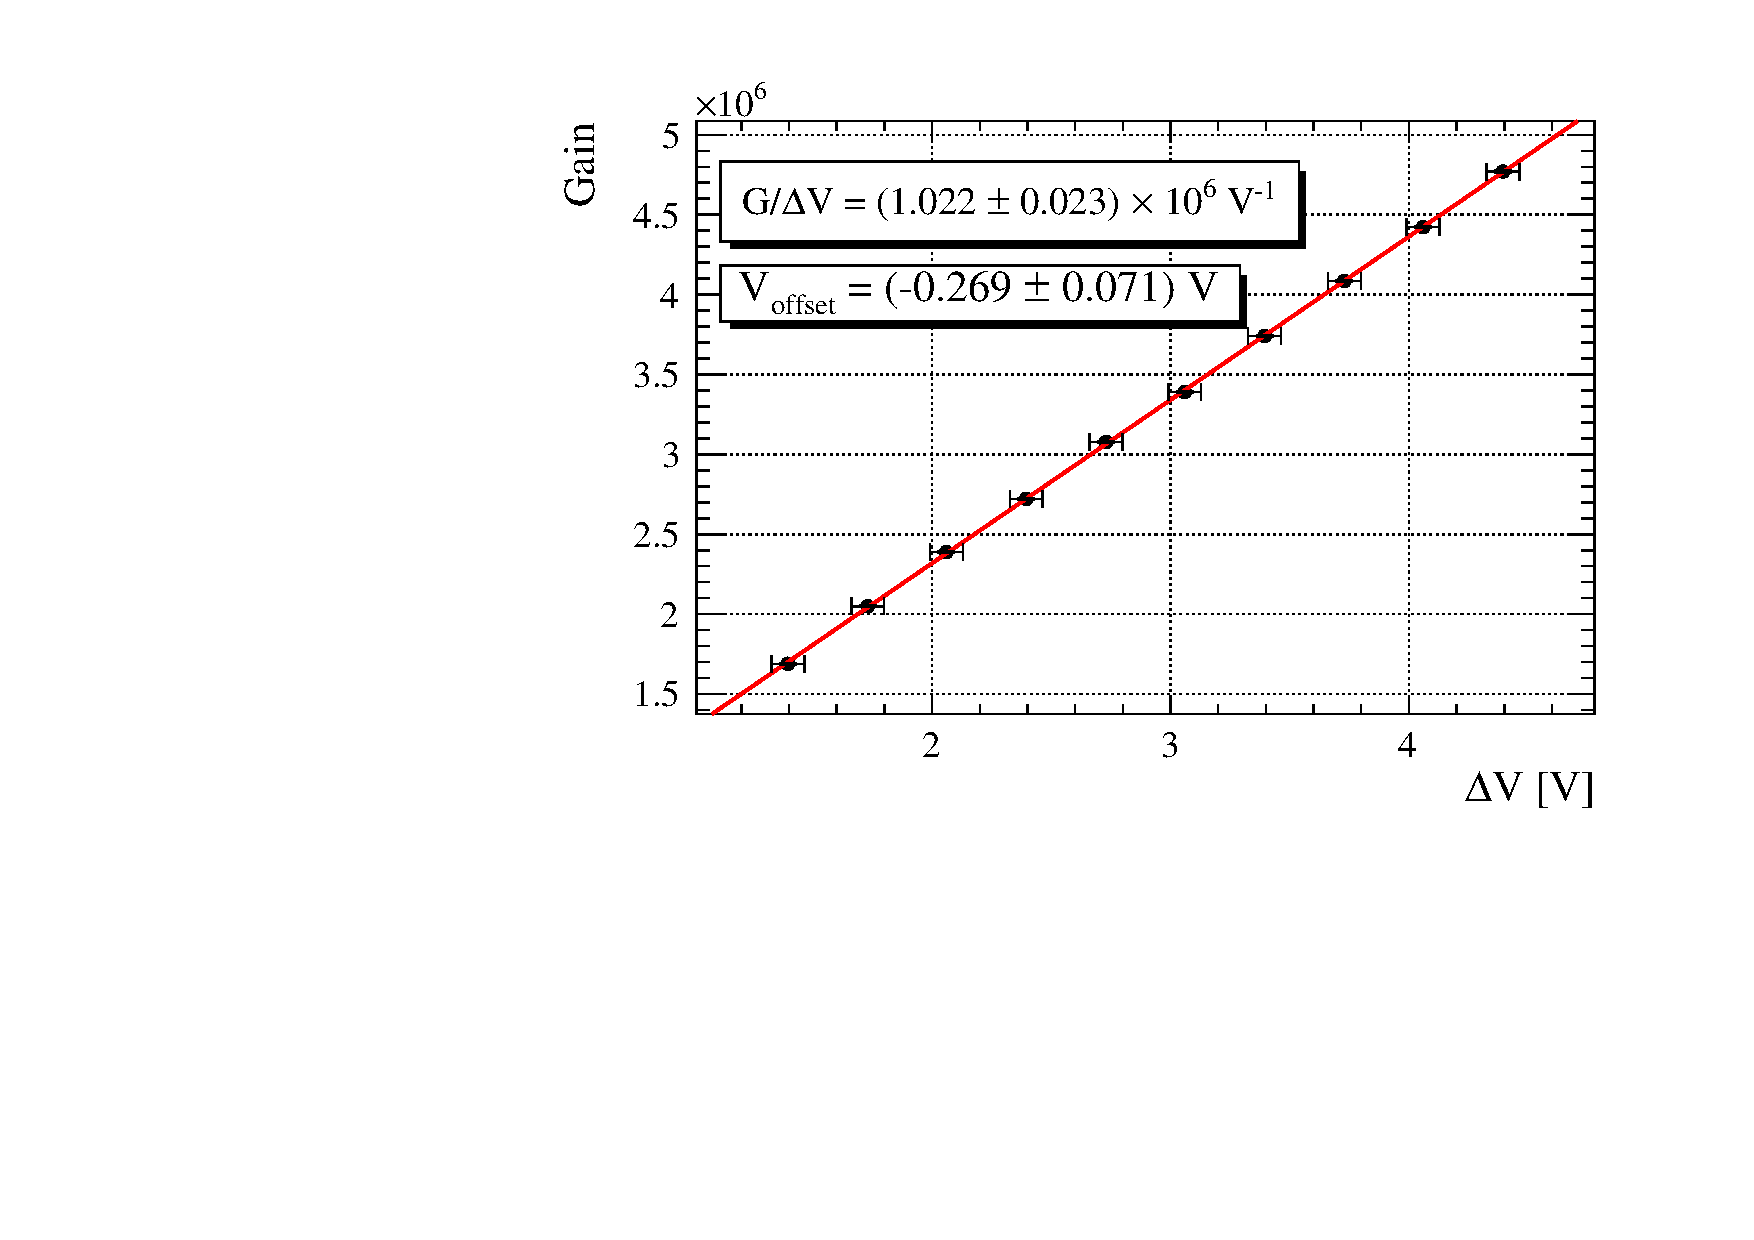
\includegraphics[width=\textwidth]{gfx/plots/Gain/H2017/Gain.pdf}
    \caption{H2017, channel $70$.}
    \label{fig:H2017 gain }
  \end{subfigure}
  \hfill
  \begin{subfigure}{0.48\textwidth}
    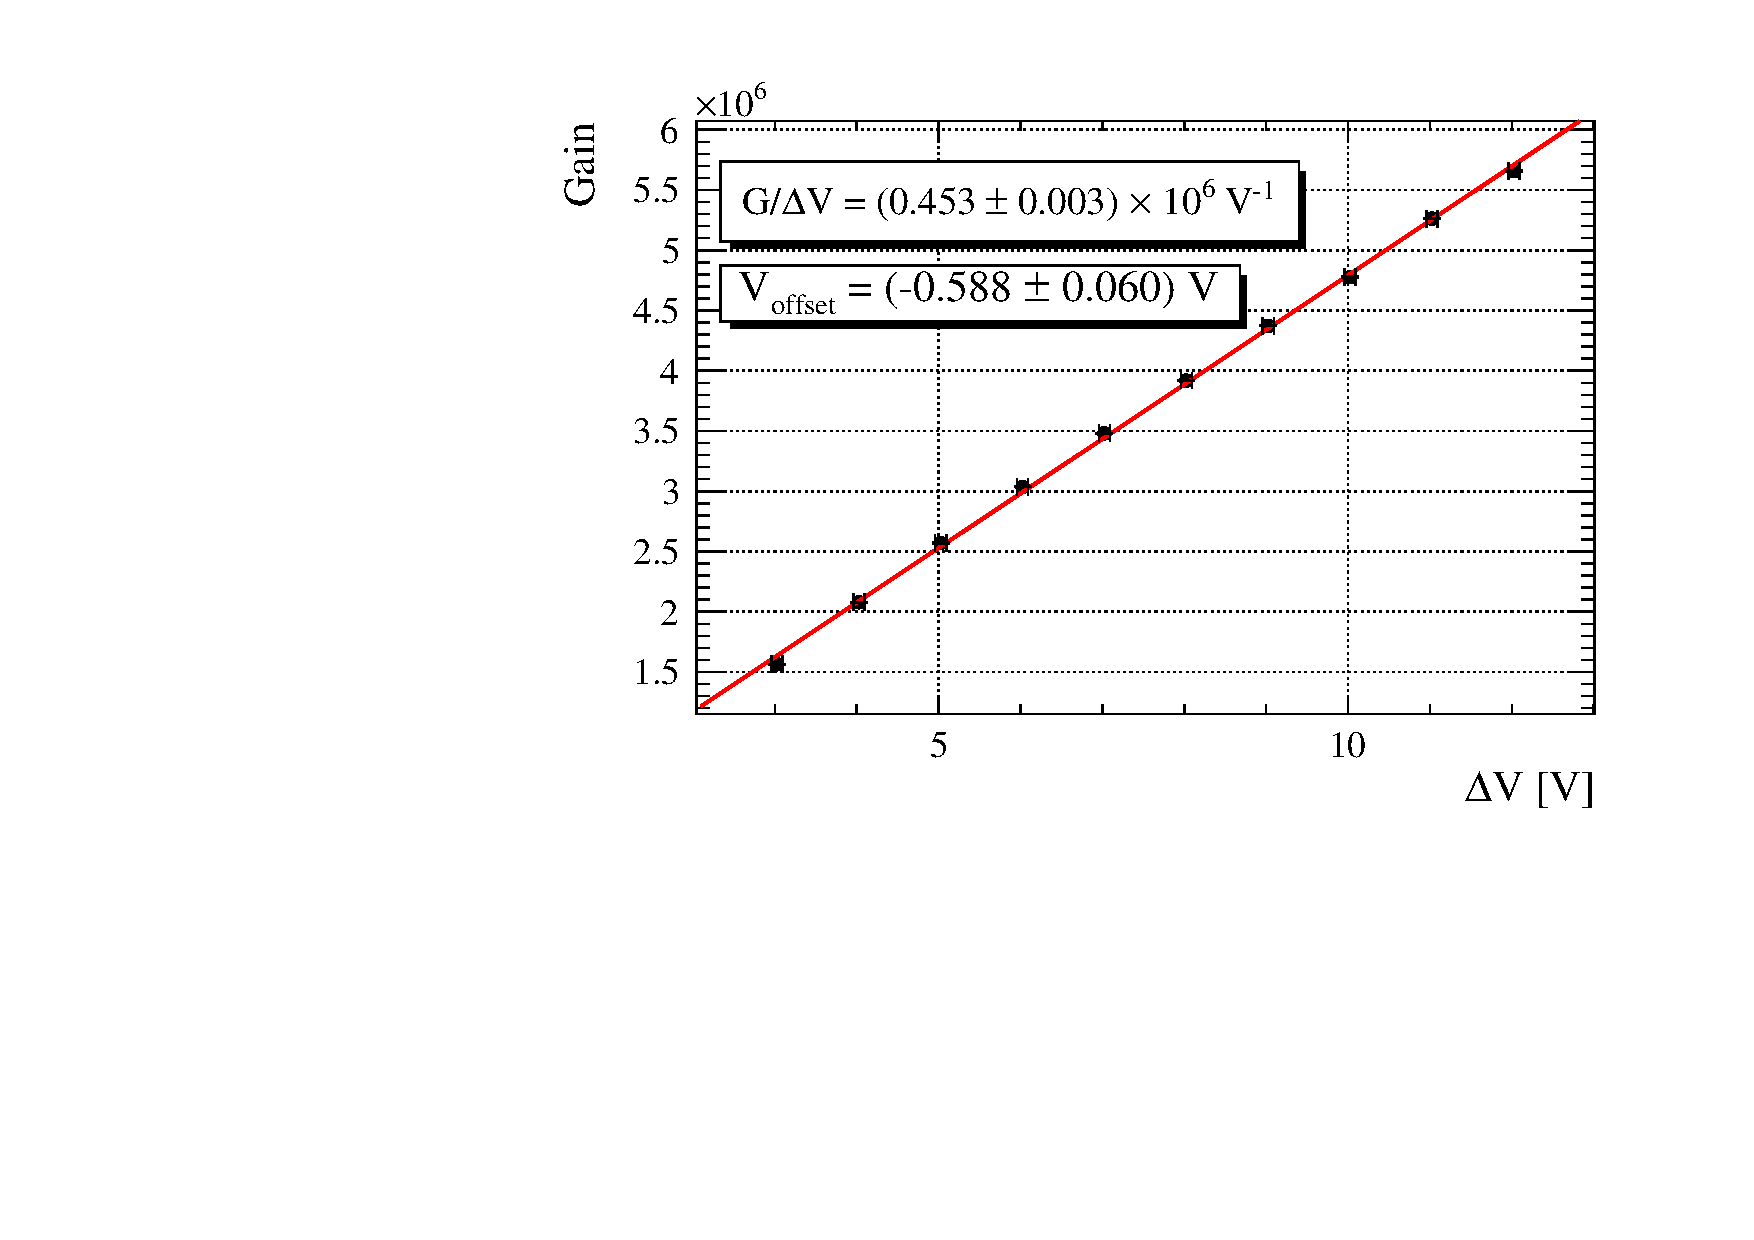
\includegraphics[width=\textwidth]{gfx/plots/Gain/31epoxy/Gain.pdf}
    \caption{FBK \SI{31}{\micro m}+ epoxy , channel $54$.}
    \label{fig:31 epoxy gain}
  \end{subfigure}
  \hfill
  \caption{Plots of the gain fit for all the studied detectors. }
  \label{fig:Gain fit for all detectors}
\end{figure}

\restoregeometry


\section{Photo-detection efficiency}
\label{ch:Results:PDE}
The PDE is measured as a function of both overvoltages and wavelengths. Measurements for $10$ different overvoltages and $50$ wavelength are performed. The PDE for the FBK \SI{16}{\micro m}, \SI{31}{\micro m}, \SI{42}{\micro m} and Hamamatsu H2017 are in Fig. \ref{fig:pde 16um}, Fig. \ref{fig:pde 31um}, Fig. \ref{fig:pde 42um} and \ref{fig:pde H2017} respectively. The PDE of the the \SI{31}{\micro m} with an epoxy layer is shown in \ref{fig:pde 31epoxy}.
On Fig. \ref{fig:pde comp epoxy} is shown for one wavelength (a) the PDE as a function of overvoltage and for one $\Delta V = 10.02$ V (b), the PDE as a function of $\lambda$ for the \SI{31}{\micro m} with and without the epoxy coating. \\
\\
The current method needs the gain measurement and then more errors are induced by this method compared to the rate. 
Is it observed that the current method underestimate the PDE relatively to the rate method by $2\%$ to $8.5\%$ of the rate PDE value at $\Delta V=12 $ V for the FBK. The maximal difference is in the \SI{42}{\micro m}. \\
\\
For the FBK bare die detectors, one can see the PDE oscillating as $\lambda$ increases. The amplitude of these oscillations is around $5\%$ of the absolute PDE value. 
One explication possible for these oscillations could be explained by optical interference in the \ac{ARC} on top of the detector. Reflected photons within the media layer could interfere constructively and destructively resulting in oscillations of the PDE. 
\\
% PDE as delta V 
As predicted by the theory, increasing the overvoltage increases the PDE but only in the operation range. Beyond, it saturates and stops increasing. This is another way of defining the operation range of the detectors. Some figures showed a decrease of the PDE by $2\%$ but this could be explained by an over correction of the noise, especially at low overvoltage where the errors in the correlated noise are bigger. 
%of a detectors and the result shown in Table. \ref{table:operation ranges}, can be confirmed or refined.
\\
%The peak sensitivity wavelength is measured of $\lambda_p = 475$nm for both current and frequency methods, which is similar to the measured $\lambda_p \approx 480$nm in \cite{Girard2018CharacterisationDistributions}. There is still a difference compared to the announced value of $450$ nm \cite{SurfaceArray}.
\\
% H2017 comparison 
Results for the Hamamatsu H2017 are shown in Fig. \ref{fig:pde H2017} and match with the measurement in  especially at high overvoltage \cite{Girard2018CharacterisationDistributions}. Some differences are noticeable, if we look at $\Delta V = 3.5$V, the maximal PDE value in \cite{Girard2018CharacterisationDistributions} is $44 \%$ whereas in \ref{fig:pde H2017}, it reaches $38\%$.
The PIN Diode calibration is a major cause of uncertainties due to errors on the calibration, also the light diffuser is not the same as in \cite{Girard2018CharacterisationDistributions}. Following this, we have not pursued these calibration uncertainties since what concerns us  for R\&D is more the differences of PDE between FBK and Hamamatsu. 
Another hint on these differences could be due the oscilloscope which has a lower band with than in \cite{Girard2018CharacterisationDistributions}. A \SI{300}{\milli V} error on $V_{bd}$ could shift the overvoltage axis (on the PDE$(\Delta V)$ plots) such that the absolute PDE value changes by several points ($1$ to $3\%$). This error is not visible on the FBK because the relative error on $V_{bd}$ is reduce due to the higher operation range.\\
\\
% epoxy talk 
In the SciFi tracker, the detectors will be installed at the output of the fibres. Since the FBK have been studied bare die, another sample of the \SI{31}{\micro m} was studied with an epoxy layer as additional coating. The results on the PDE are visible on Fig. \ref{fig:pde 31epoxy} and one can clearly see that the oscillations are cancelled. %The peak sensitivity for the FBK NUV-HD is announced around $\lambda_p= 400$nm \cite{} and the measurement are partially in agreement with this, even though measurement below $400$nm should be done to confirm it. Nevertheless, since the light coming from the SciFi is not below $400$nm, this information is not relevant for us. 
One can notice on the plots of the PDE as a function of $\Delta V$ (left plot) that at very high $\Delta V$, the efficiency saturates reaching a maximal value of $45\%$ at $\Delta V=12 $ V. The comparison with the bare die detector and with the epoxy layer for one overvoltage is shown in Fig. \ref{fig:pde comp epoxy}. We notice that the epoxy version behaves as the mean value of the oscillations. 
% general comments about SiPMs
It is observed that the detectors with smaller pixels has a smaller PDE because of their lower FF. 

\newgeometry{left=0.5cm,right=0.5cm,top=1.5cm,bottom=1.5cm}
\begin{landscape}
\begin{figure}[htbp]
    \centering
    \begin{subfigure}{0.65\textwidth}
        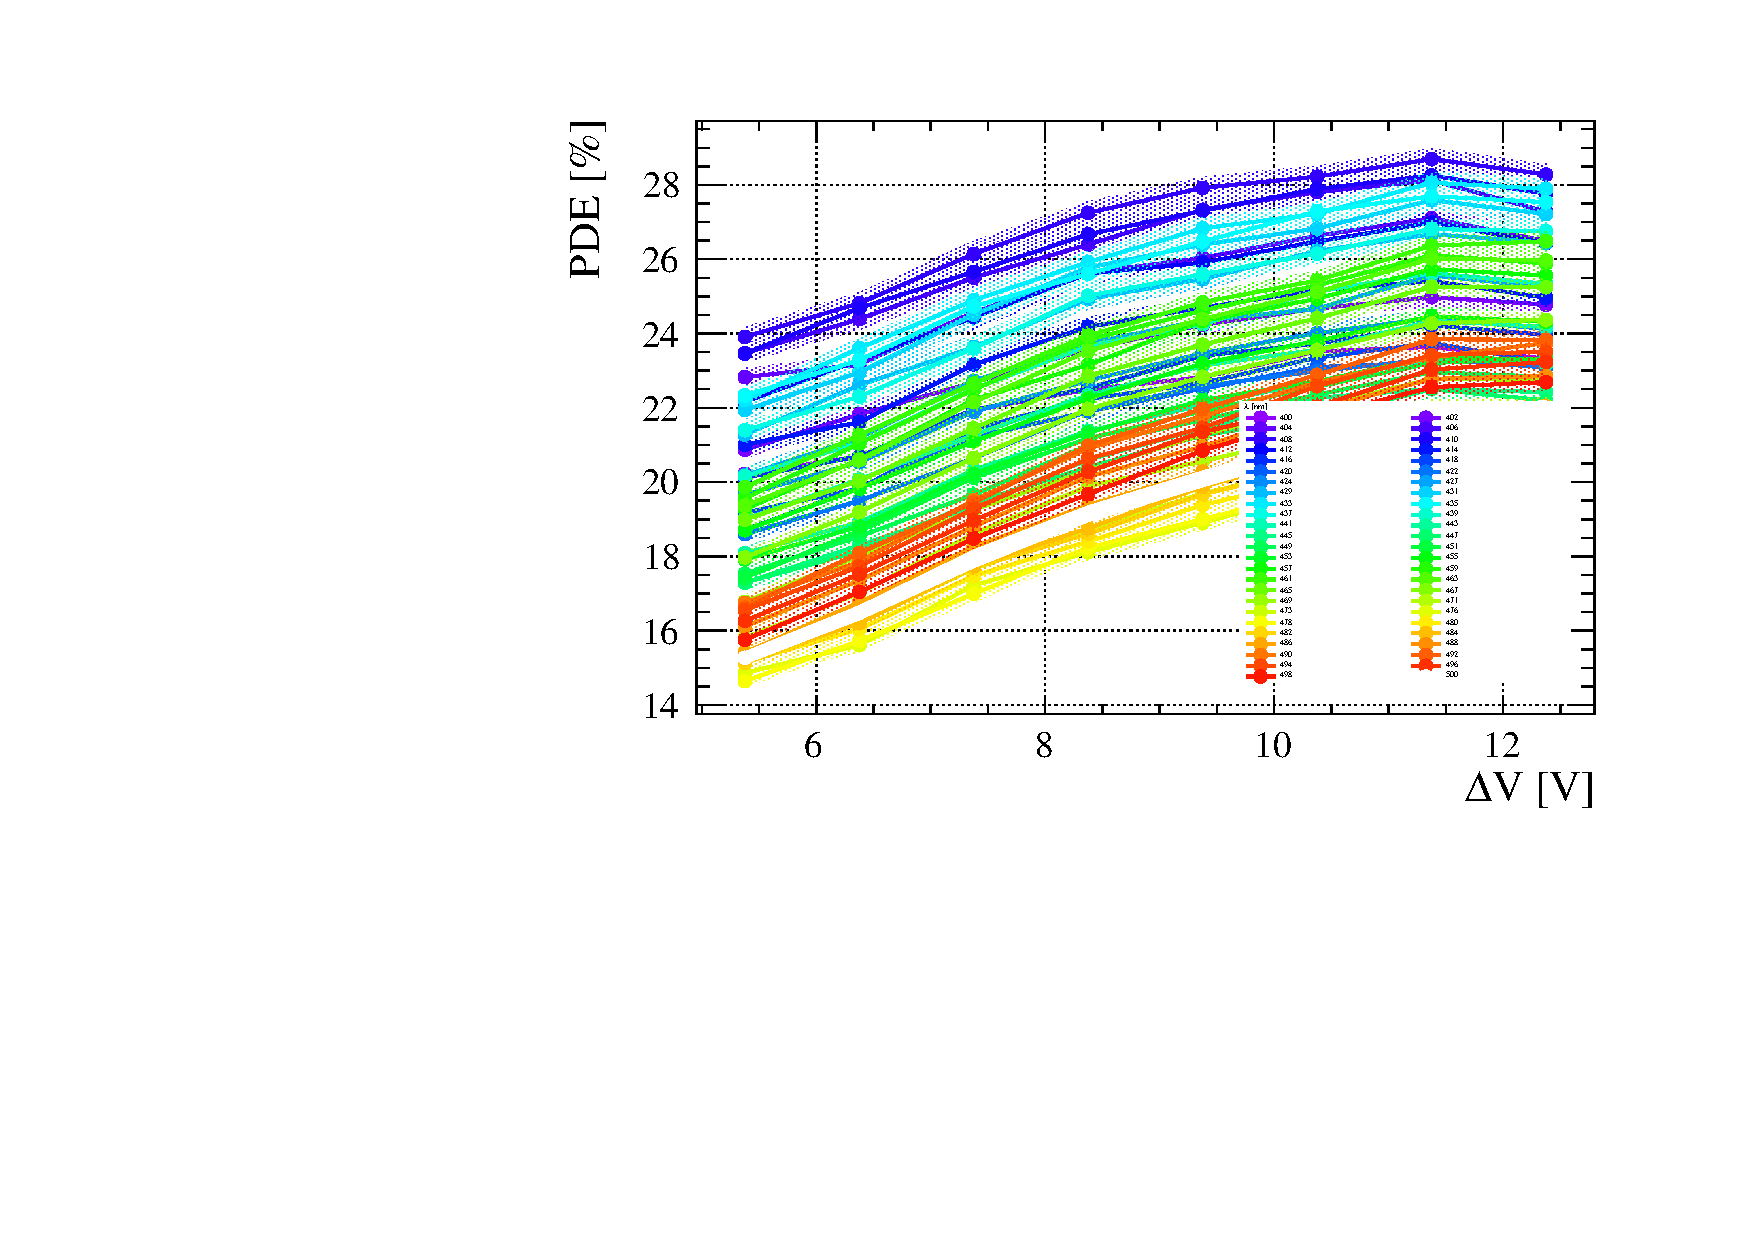
\includegraphics[width=\linewidth]{gfx/plots/PDE/16/c_Current_Bias.pdf}  
        \caption{Current}
    \end{subfigure}
    %\hfill
    \begin{subfigure}{0.65\textwidth}
        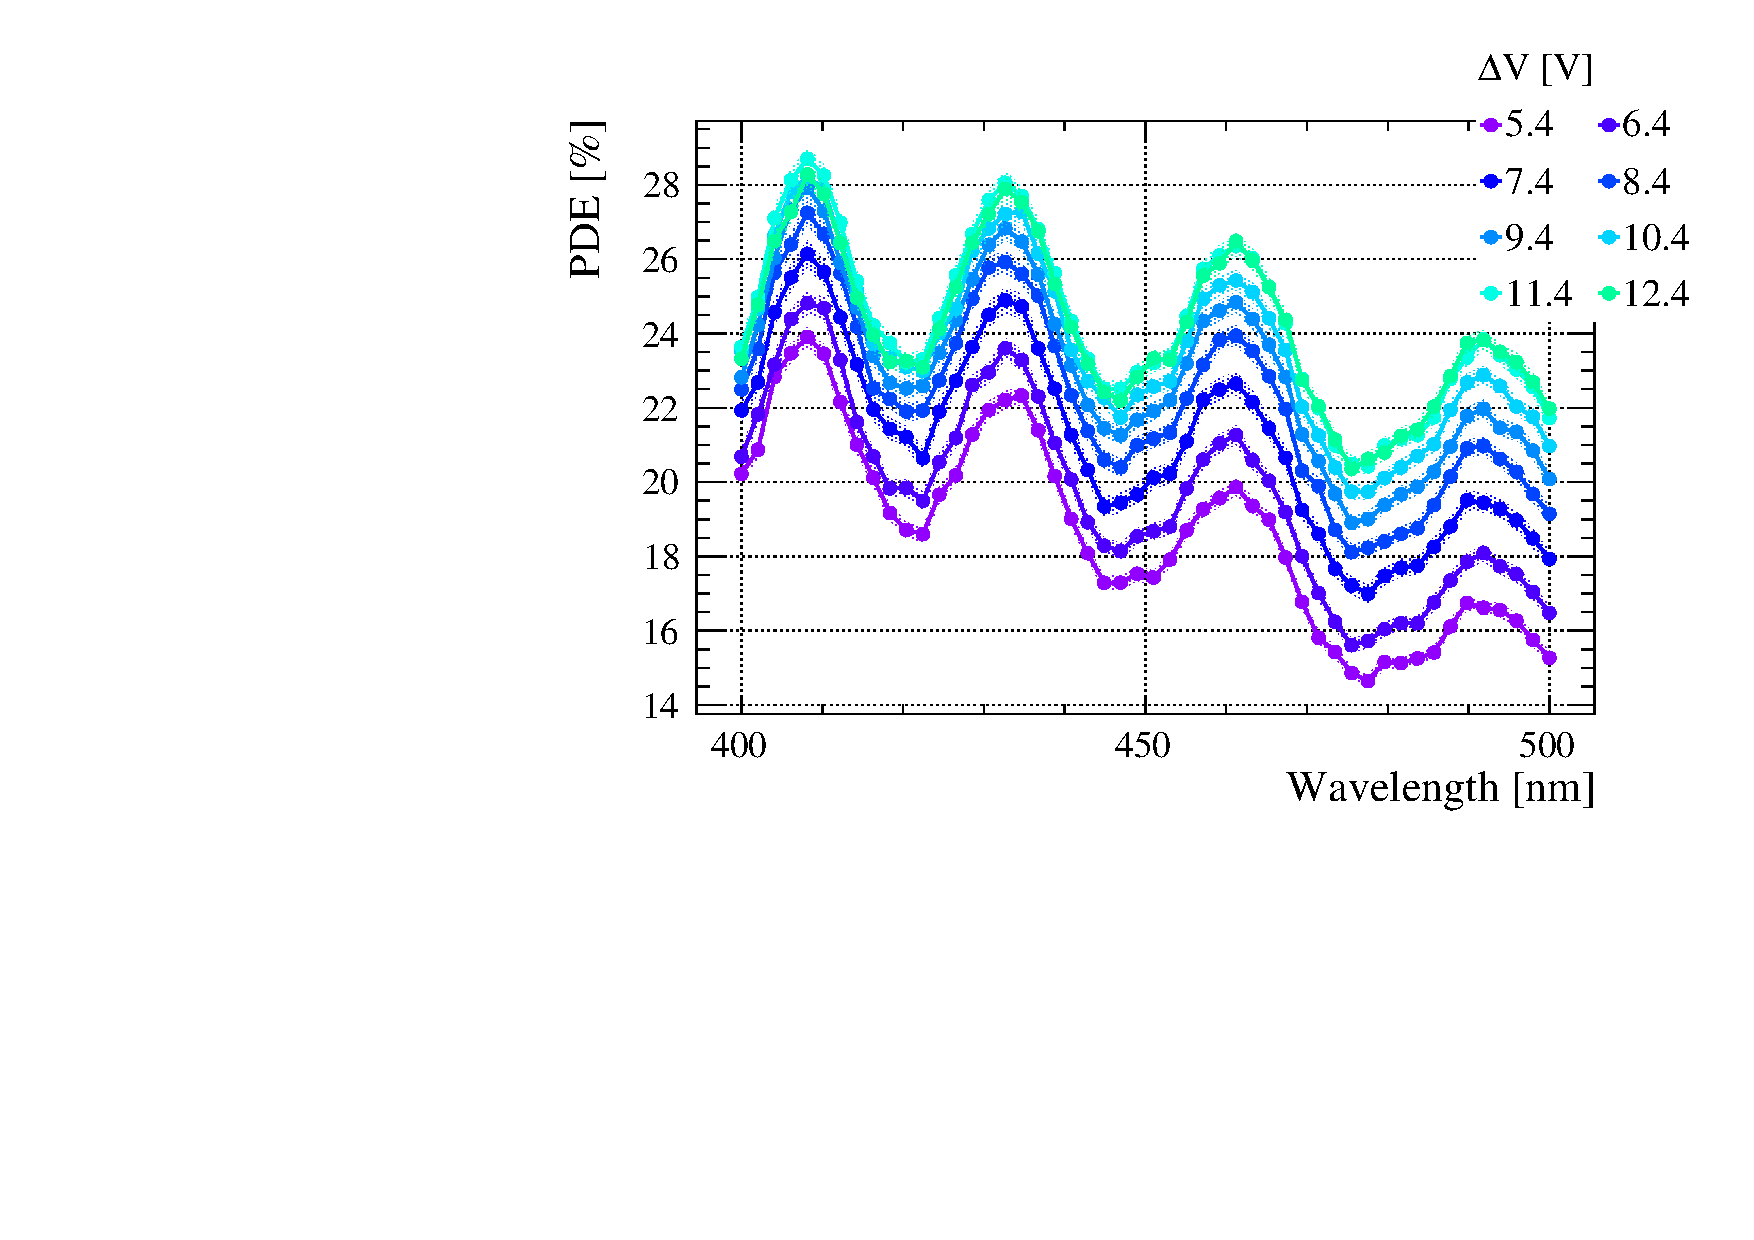
\includegraphics[width=\linewidth]{gfx/plots/PDE/16/c_Current_Wavelength.pdf}  
        \caption{Current}
    \end{subfigure}
    \\
    \begin{subfigure}{0.65\textwidth}
        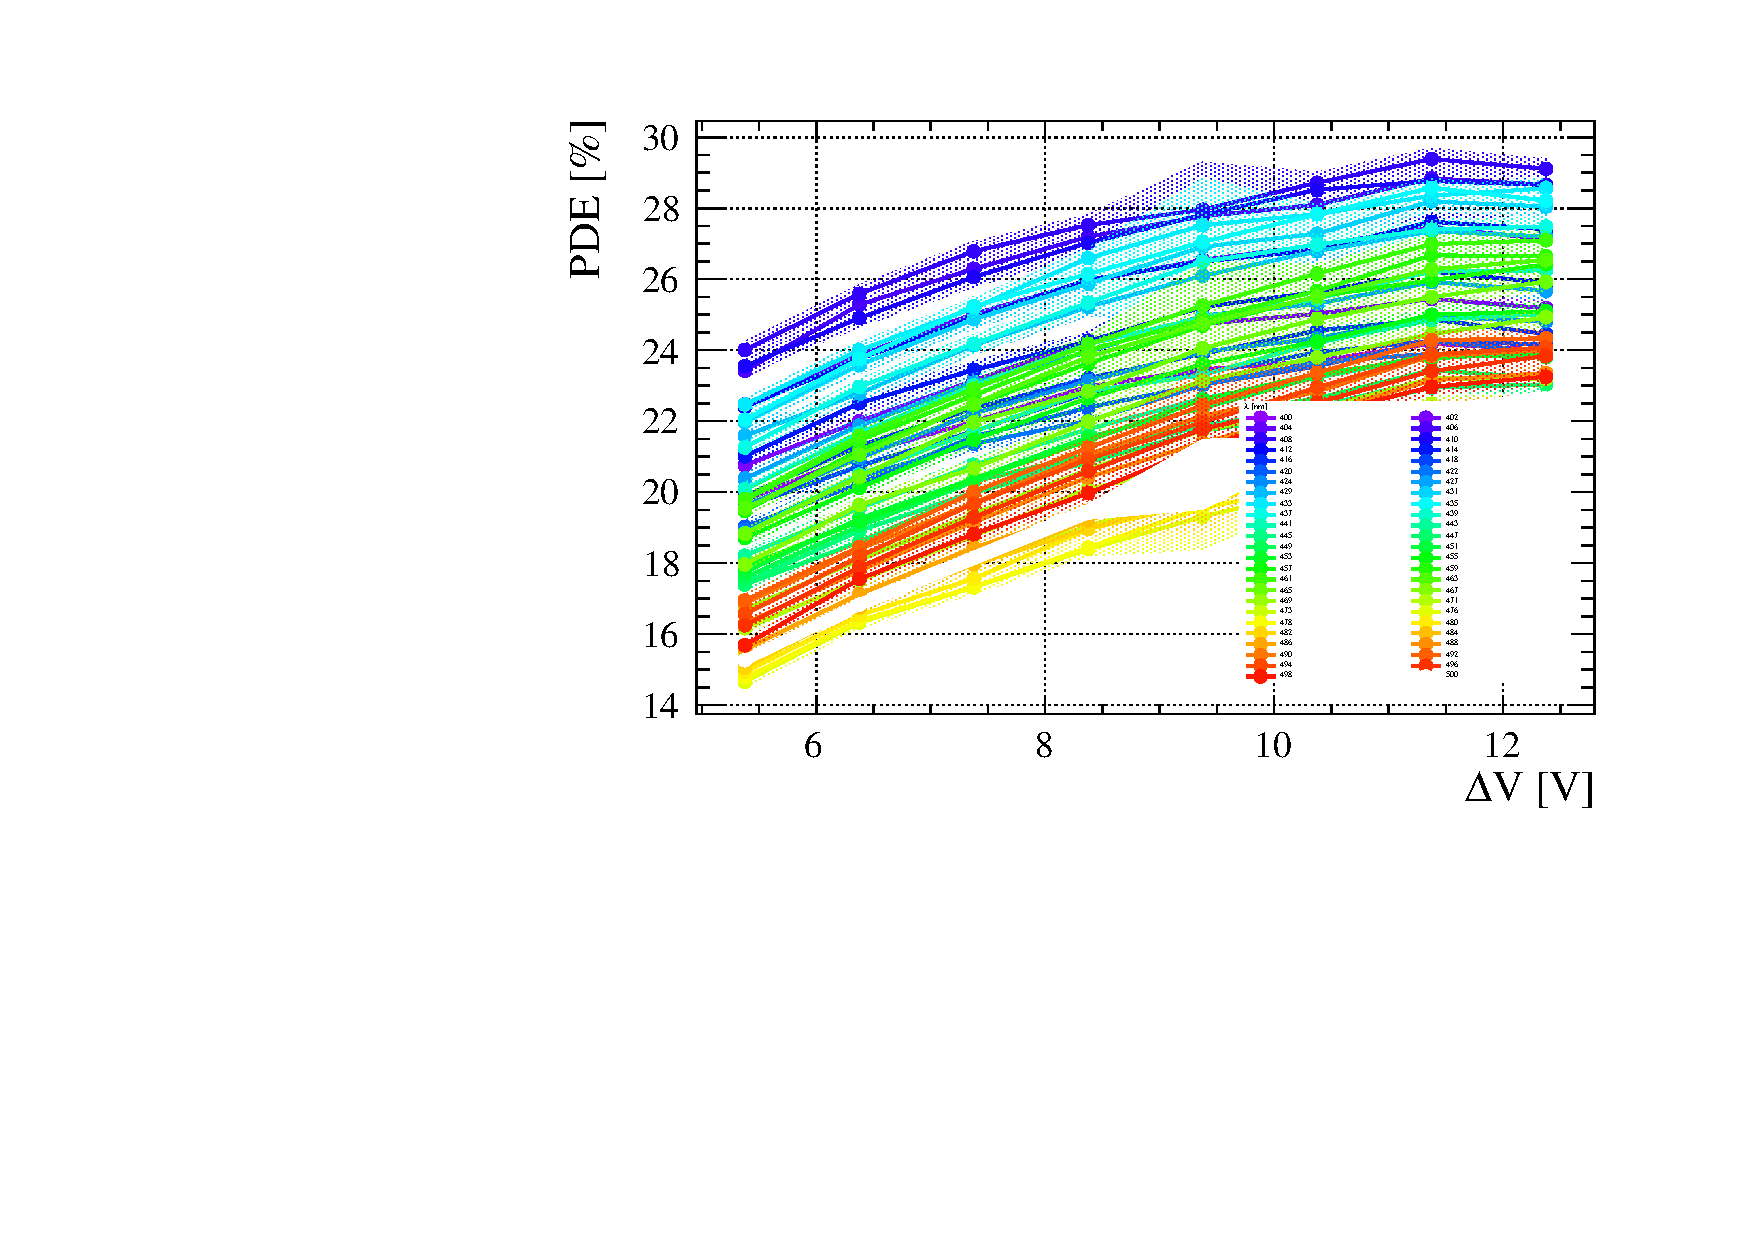
\includegraphics[width=\linewidth]{gfx/plots/PDE/16/c_Freq_Bias.pdf}    
        \caption{Rate}
    \end{subfigure}
    %\hfill
    \begin{subfigure}{0.65\textwidth}
        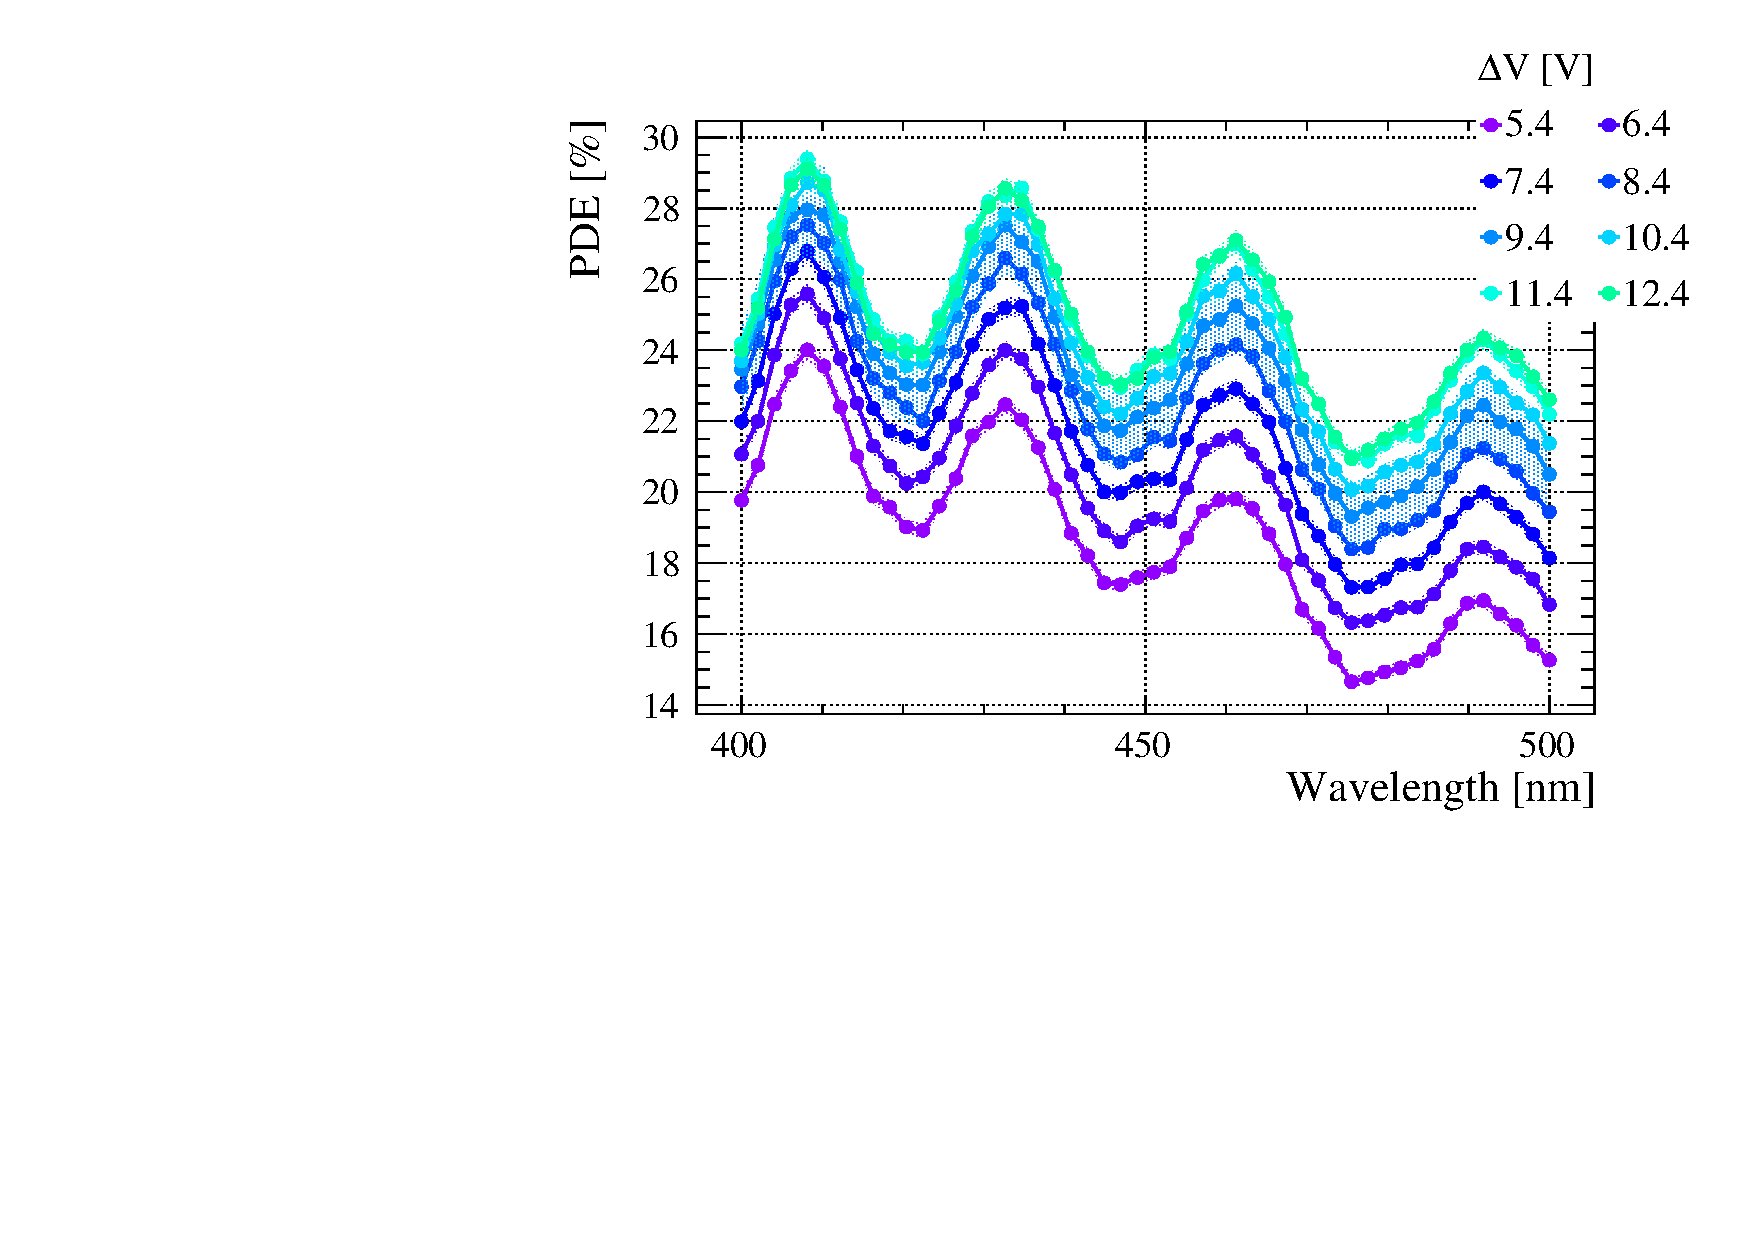
\includegraphics[width=\linewidth]{gfx/plots/PDE/16/c_Freq_Wavelength.pdf} 
        \caption{Rate}
    \end{subfigure}
    \caption{PDE of the FBK \SI{16}{\micro m}.}
    \label{fig:pde 16um}
\end{figure}

\end{landscape}

\begin{landscape}
\begin{figure}[htbp]
    \centering
    \begin{subfigure}{0.65\textwidth}
        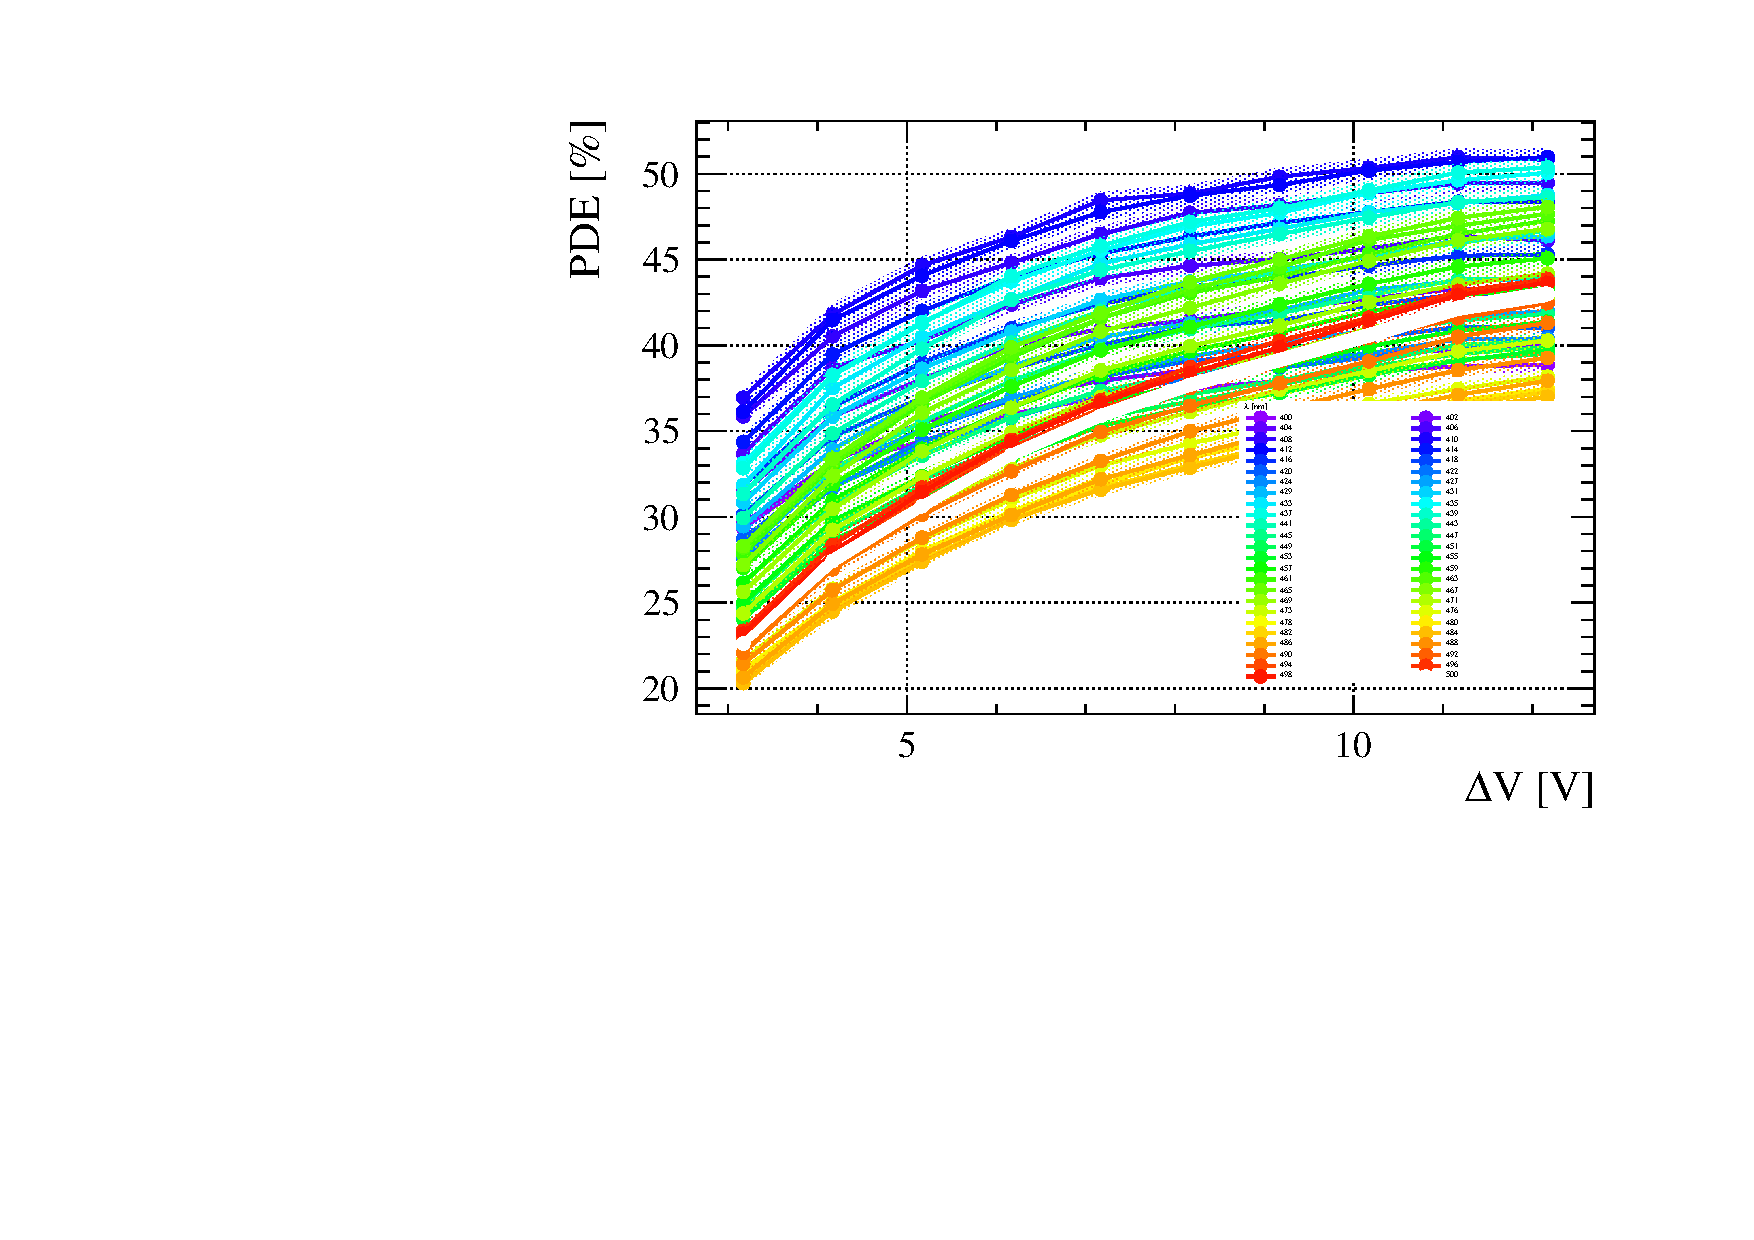
\includegraphics[width=\linewidth]{gfx/plots/PDE/31/c_Current_Bias.pdf}  
        \caption{Current}
    \end{subfigure}
    %\hfill
    \begin{subfigure}{0.65\textwidth}
        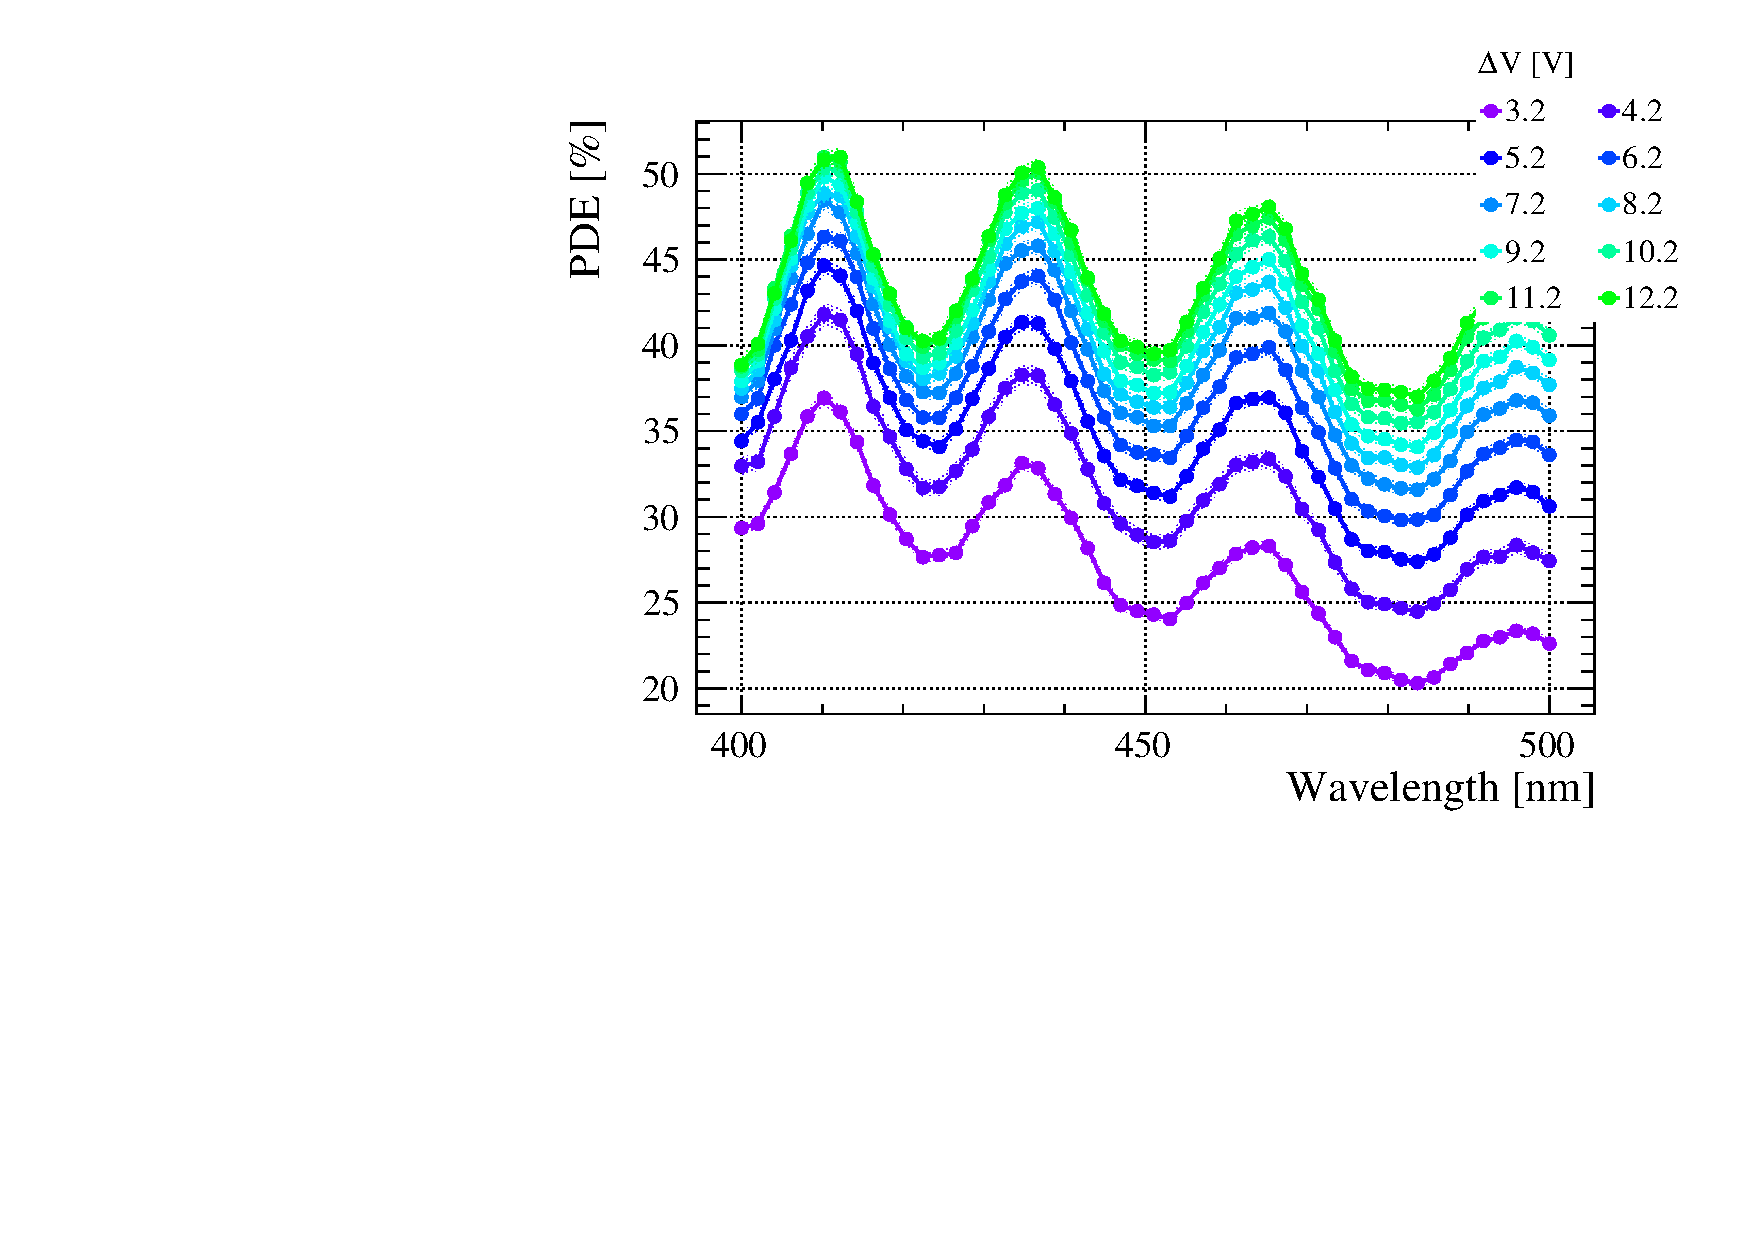
\includegraphics[width=\linewidth]{gfx/plots/PDE/31/c_Current_Wavelength.pdf}  
        \caption{Current}
    \end{subfigure}
    \\
    \begin{subfigure}{0.65\textwidth}
        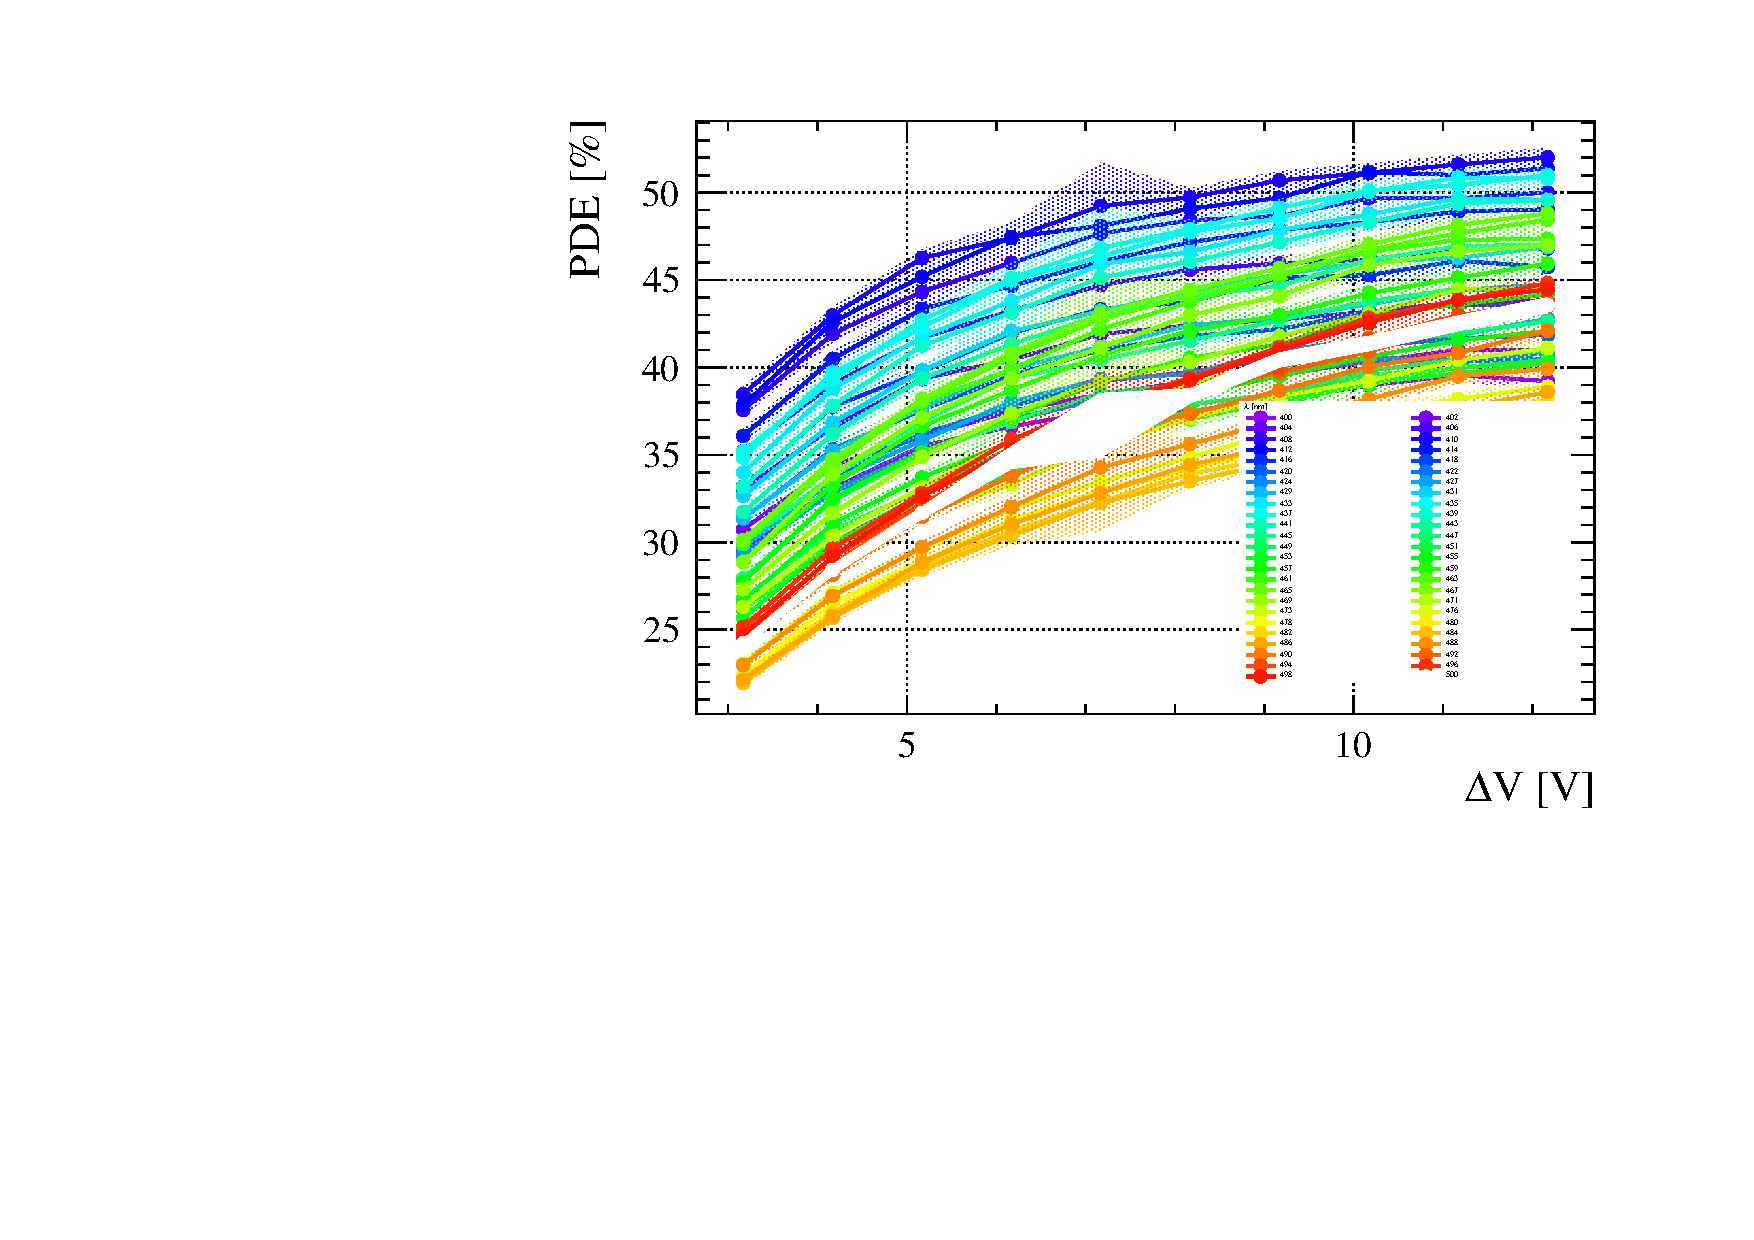
\includegraphics[width=\linewidth]{gfx/plots/PDE/31/c_Freq_Bias.pdf}    
        \caption{Rate}
    \end{subfigure}
    %\hfill
    \begin{subfigure}{0.65\textwidth}
        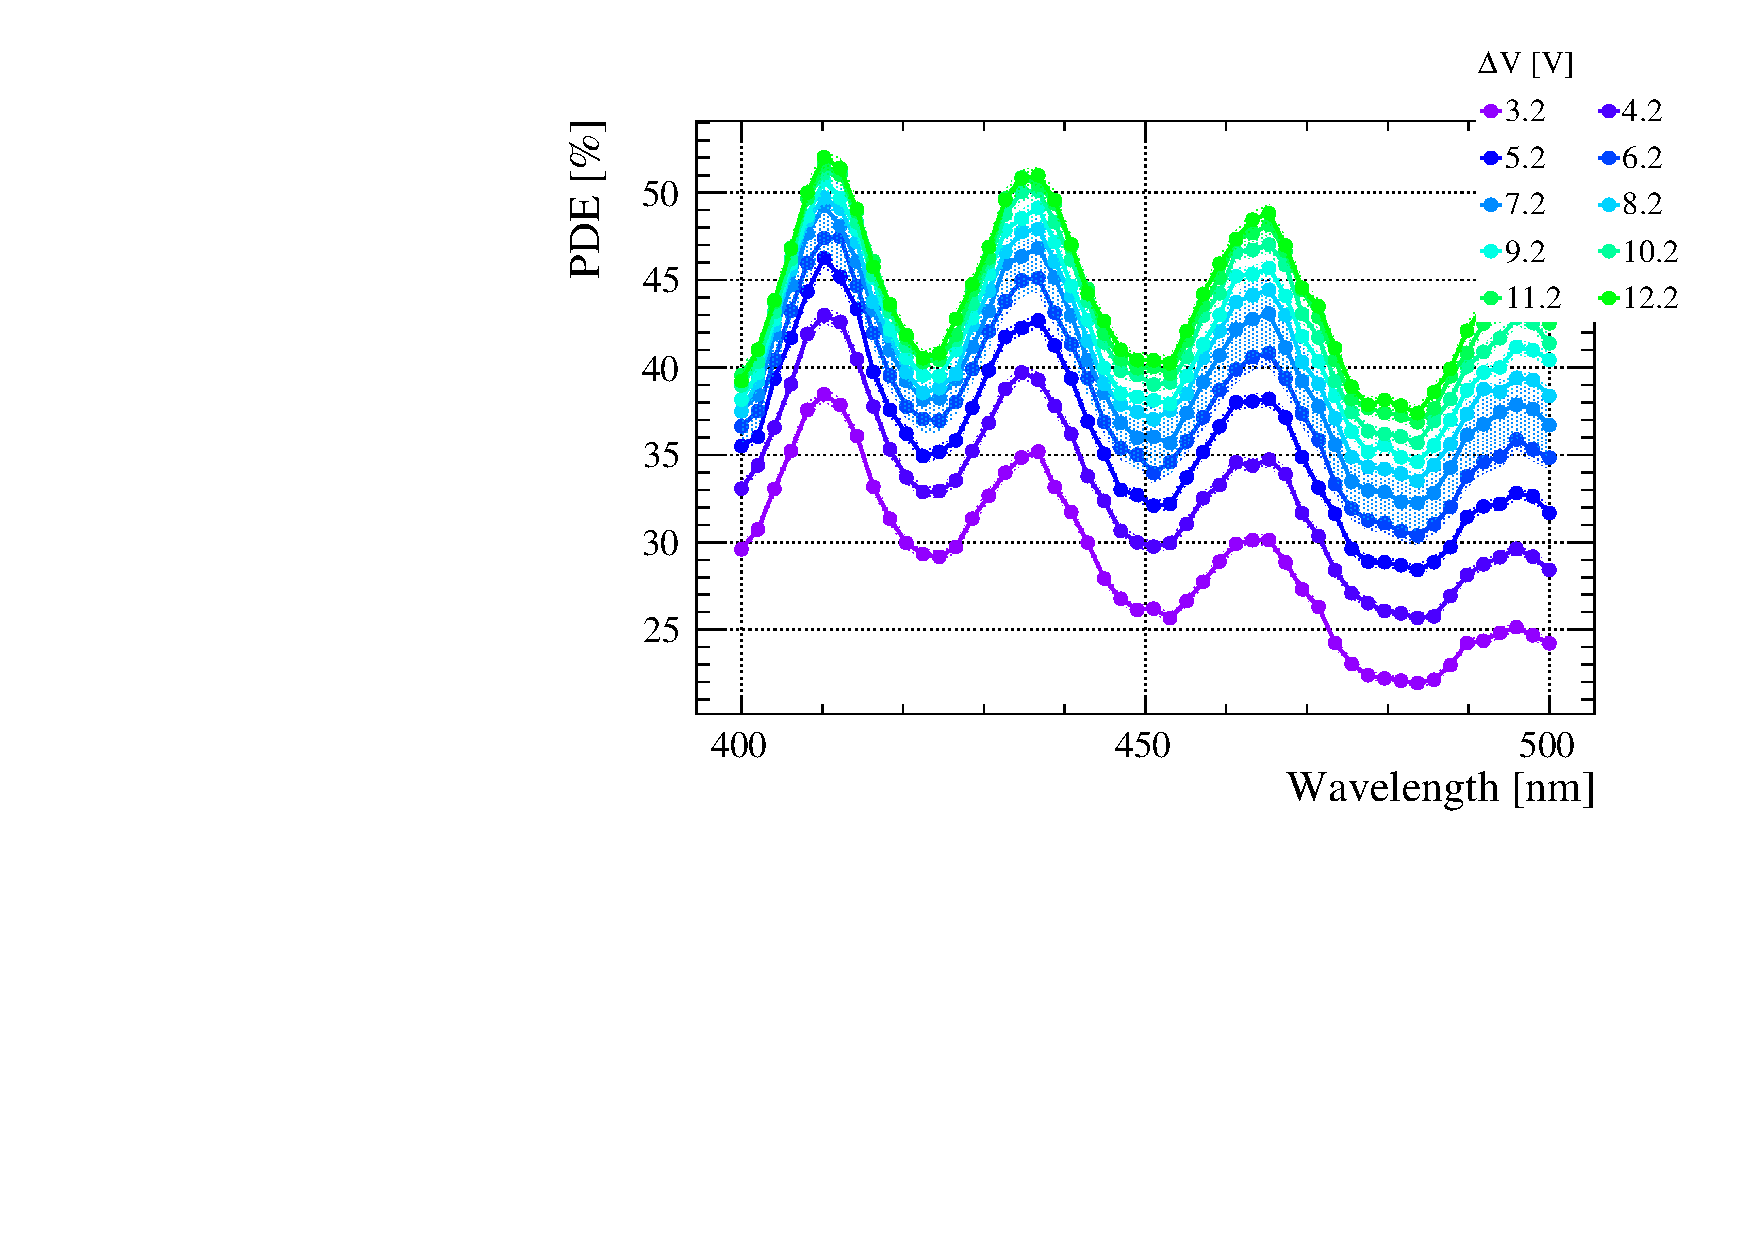
\includegraphics[width=\linewidth]{gfx/plots/PDE/31/c_Freq_Wavelength.pdf} 
        \caption{Rate}
    \end{subfigure}
    \caption{PDE of the FBK \SI{31}{\micro m}.}
    \label{fig:pde 31um}
\end{figure}
\end{landscape}

\begin{landscape}  
\begin{figure}[htbp]
    \centering
    \begin{subfigure}{0.65\textwidth}
        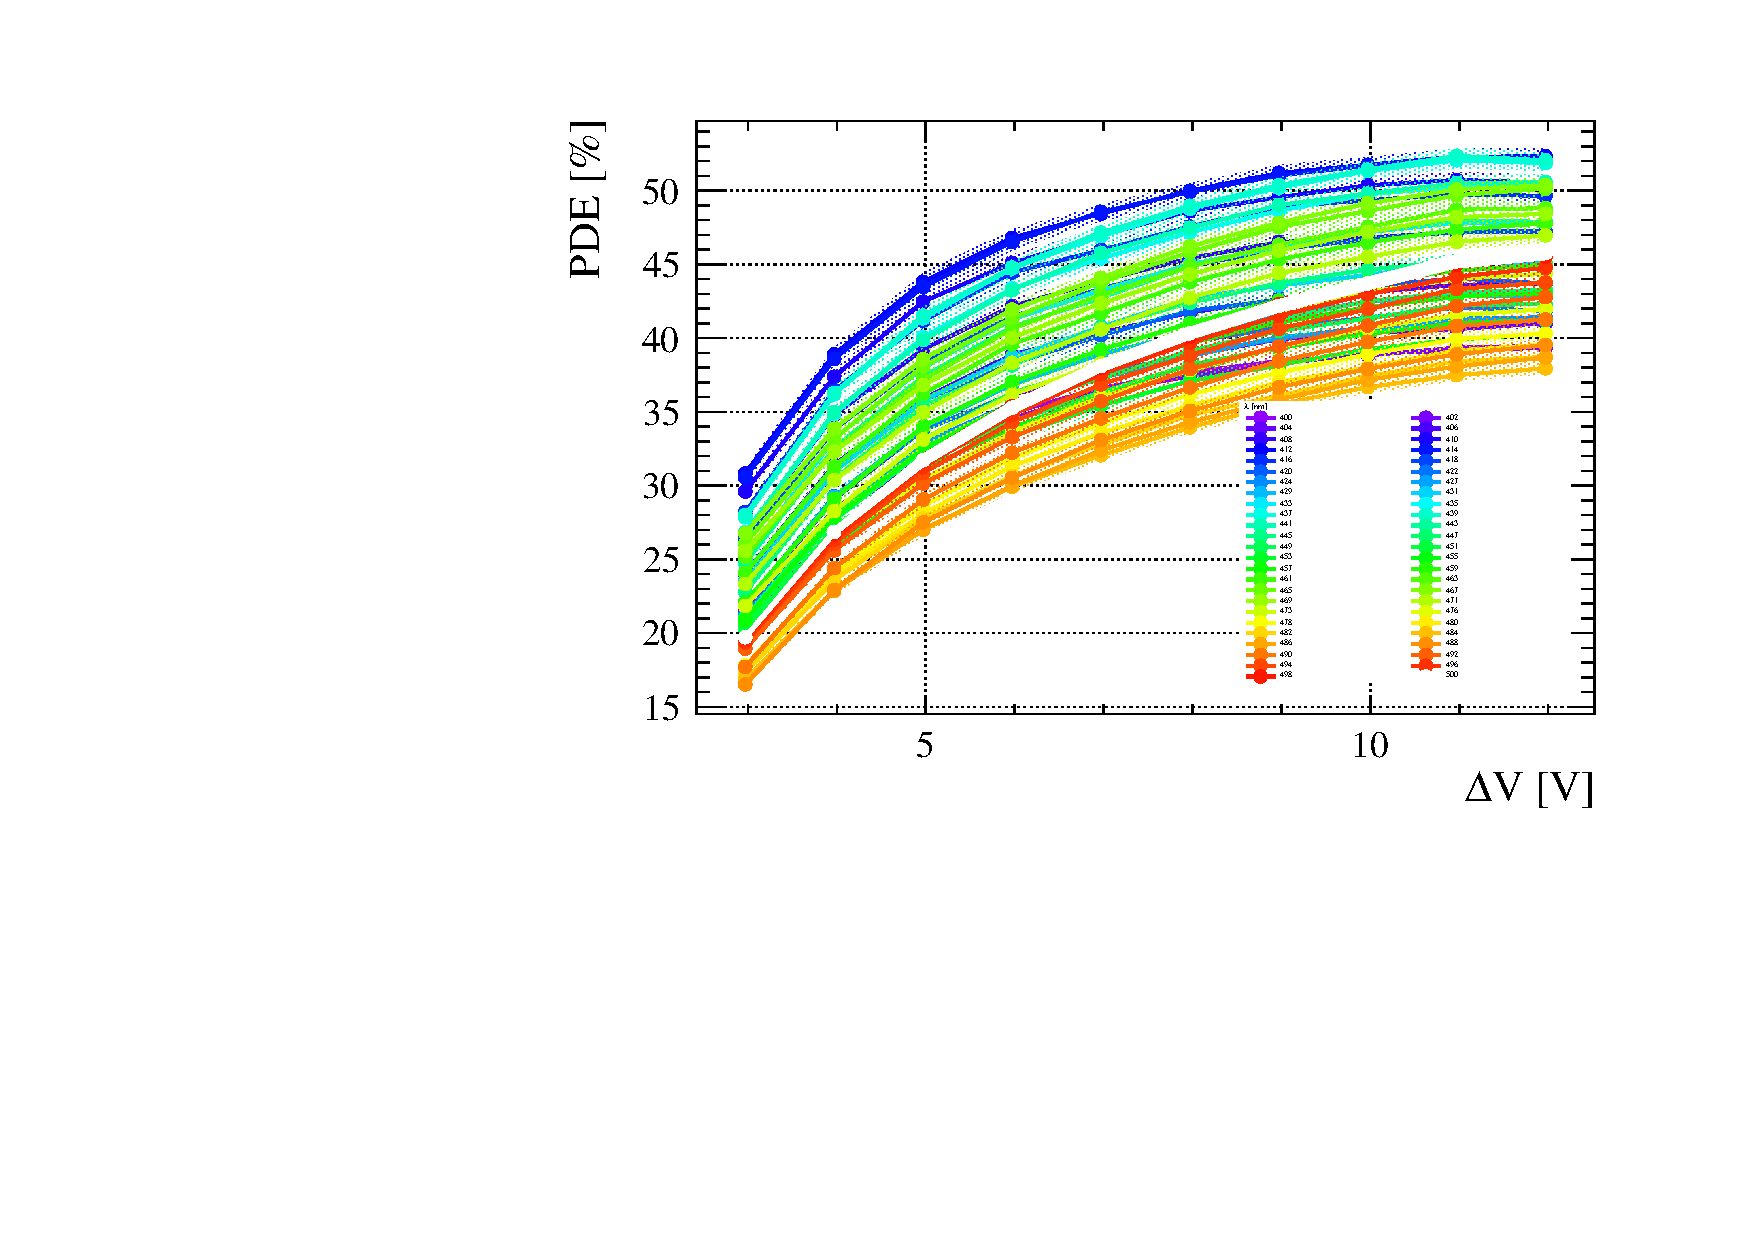
\includegraphics[width=\linewidth]{gfx/plots/PDE/42/c_Current_Bias.pdf}  
        \caption{Current}
    \end{subfigure}
    %\hfill
    \begin{subfigure}{0.65\textwidth}
        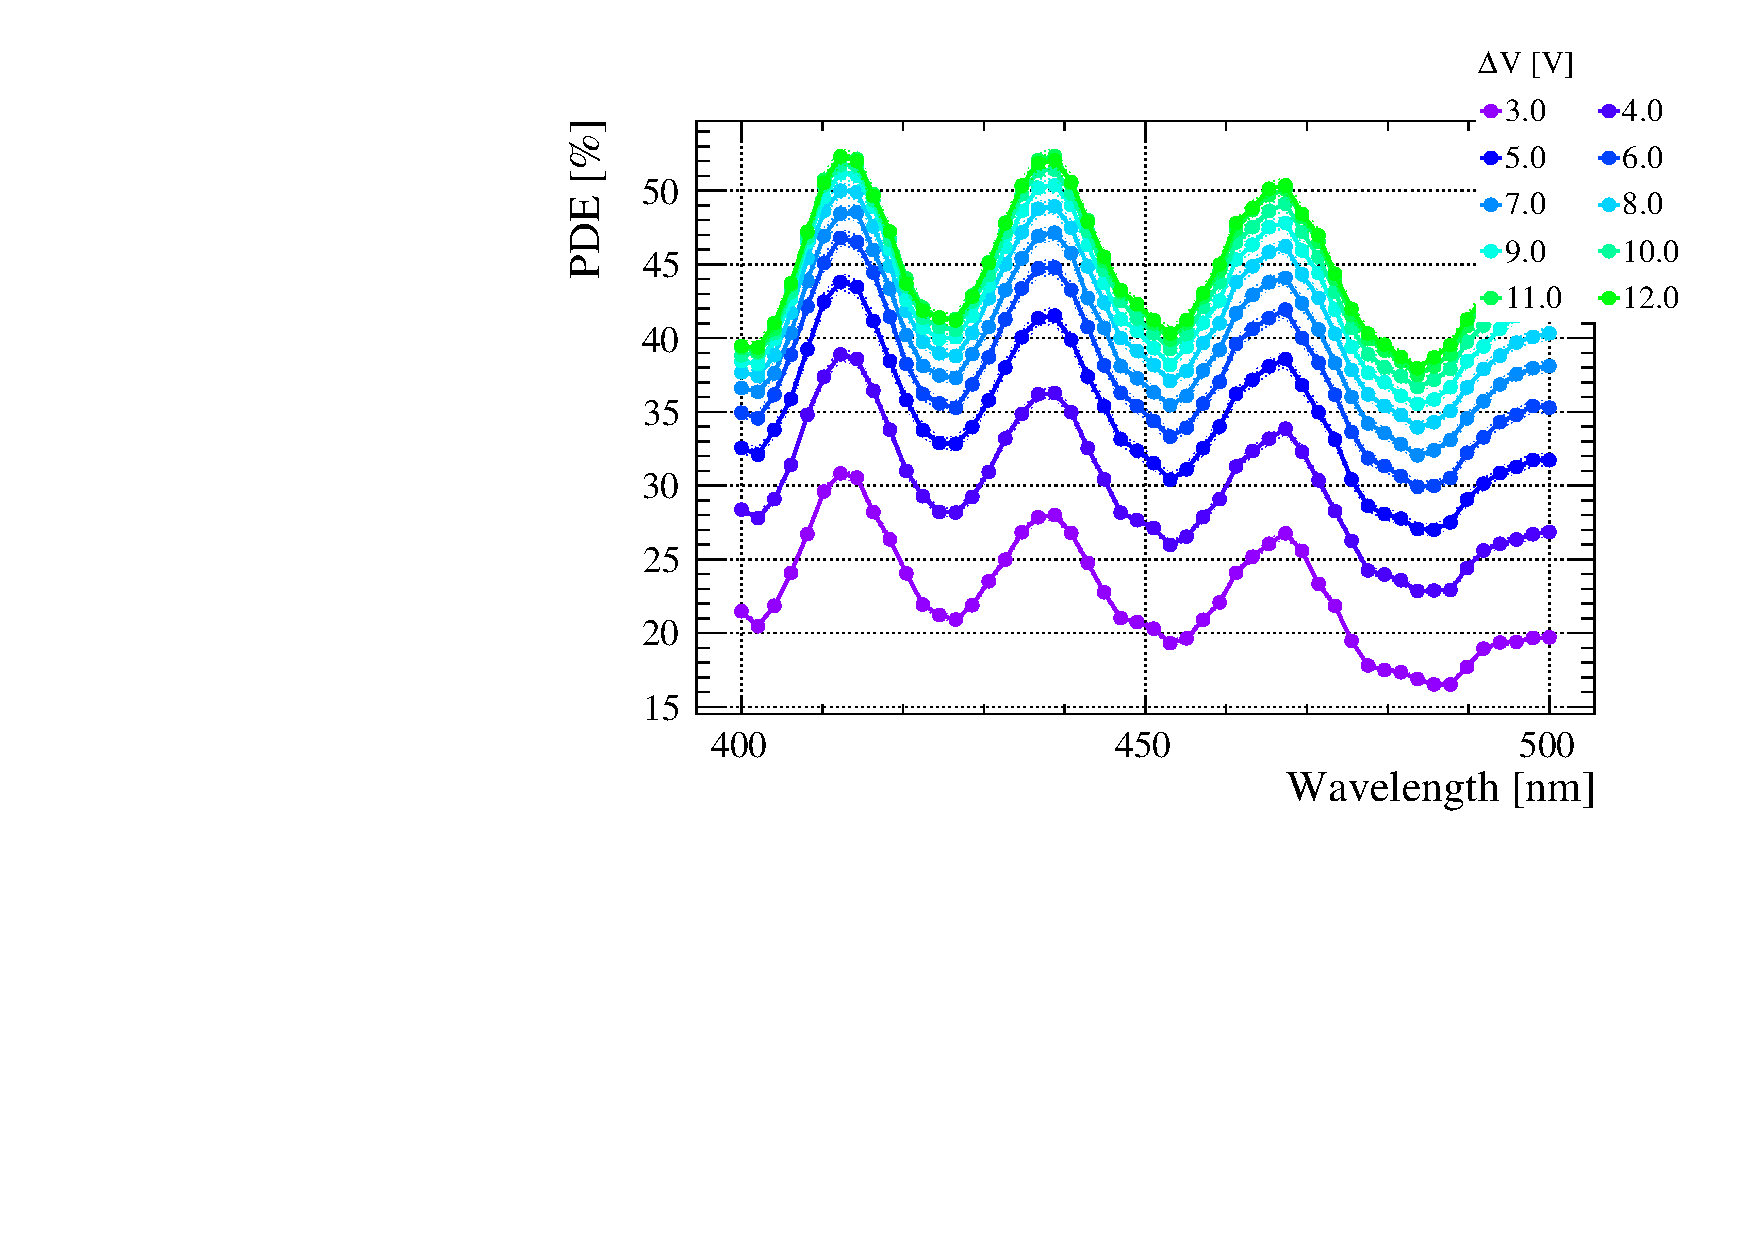
\includegraphics[width=\linewidth]{gfx/plots/PDE/42/c_Current_Wavelength.pdf}  
        \caption{Current}
    \end{subfigure}
    \\
    \begin{subfigure}{0.65\textwidth}
        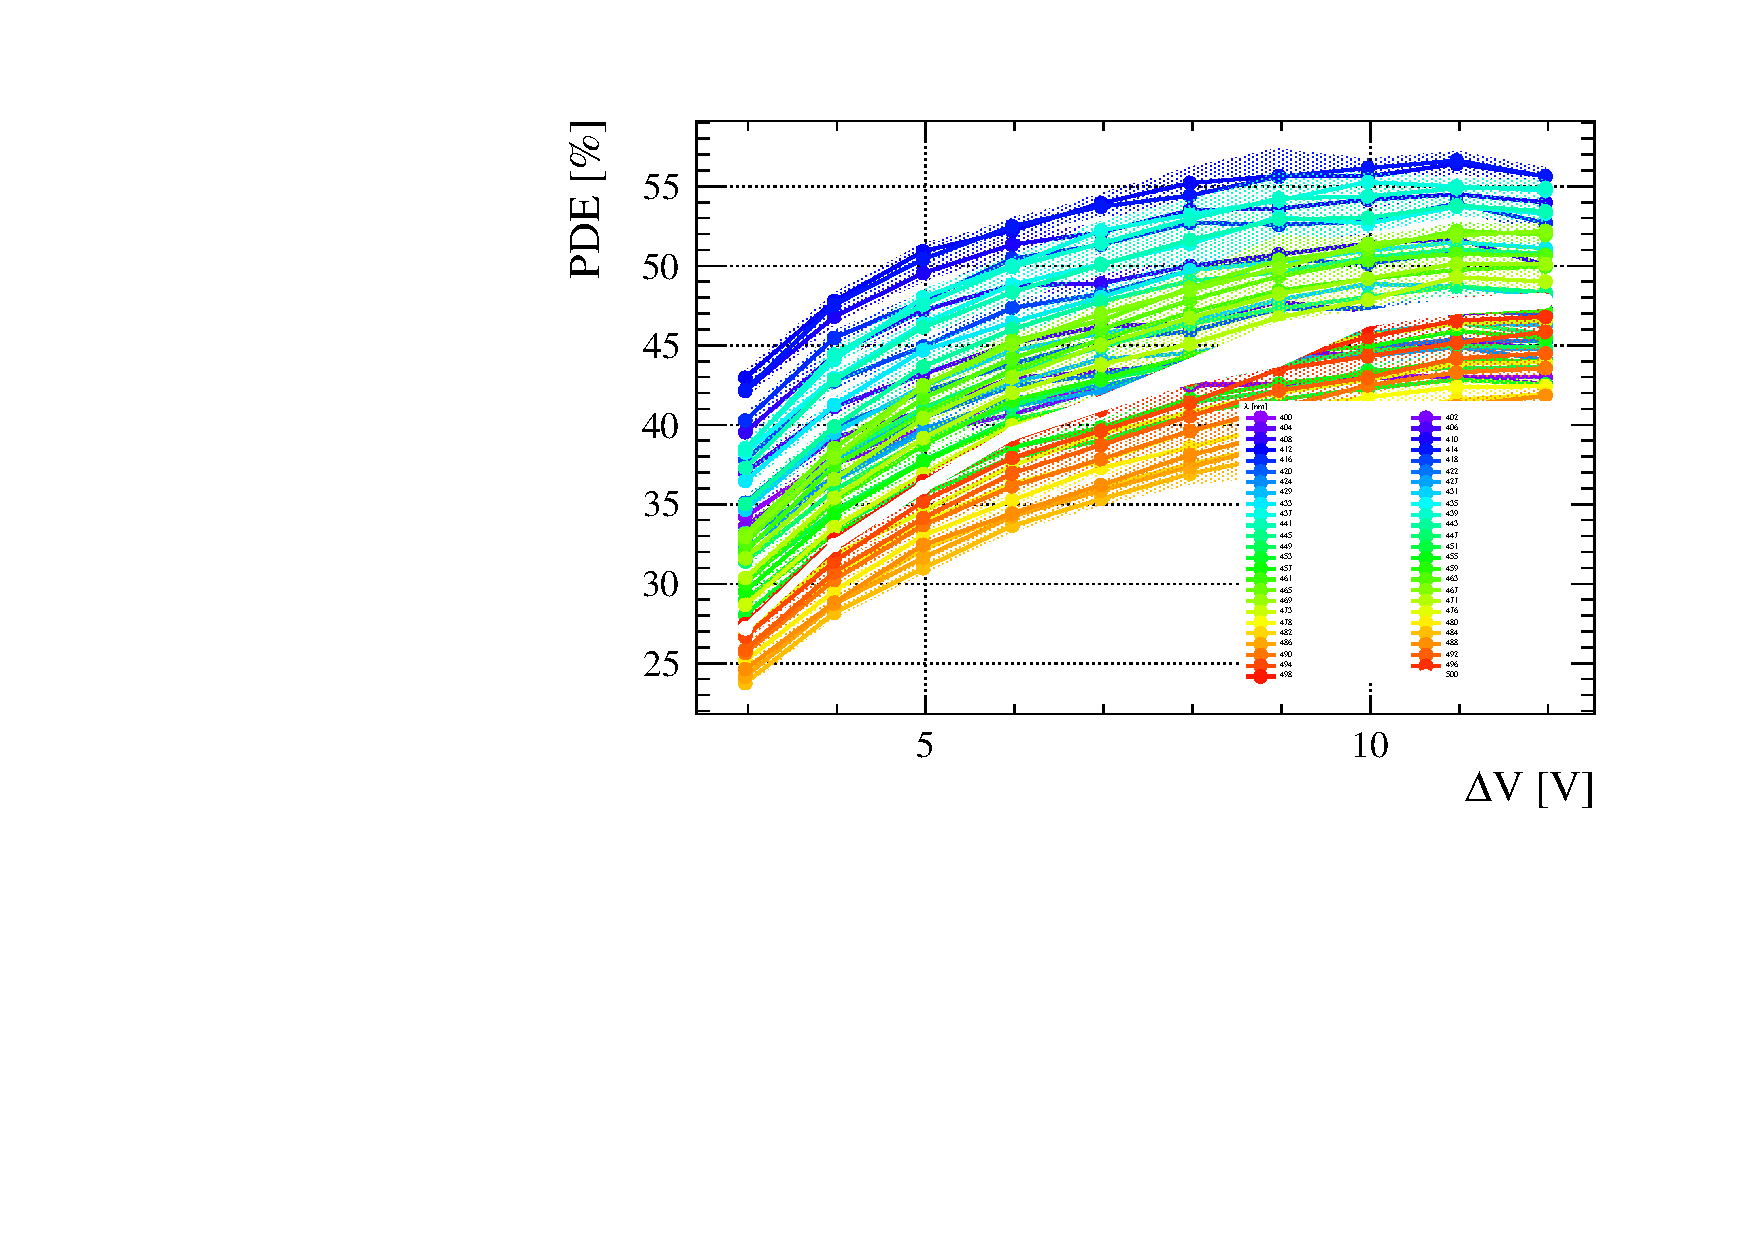
\includegraphics[width=\linewidth]{gfx/plots/PDE/42/c_Freq_Bias.pdf}    
        \caption{Rate}
    \end{subfigure}
    %\hfill
    \begin{subfigure}{0.65\textwidth}
        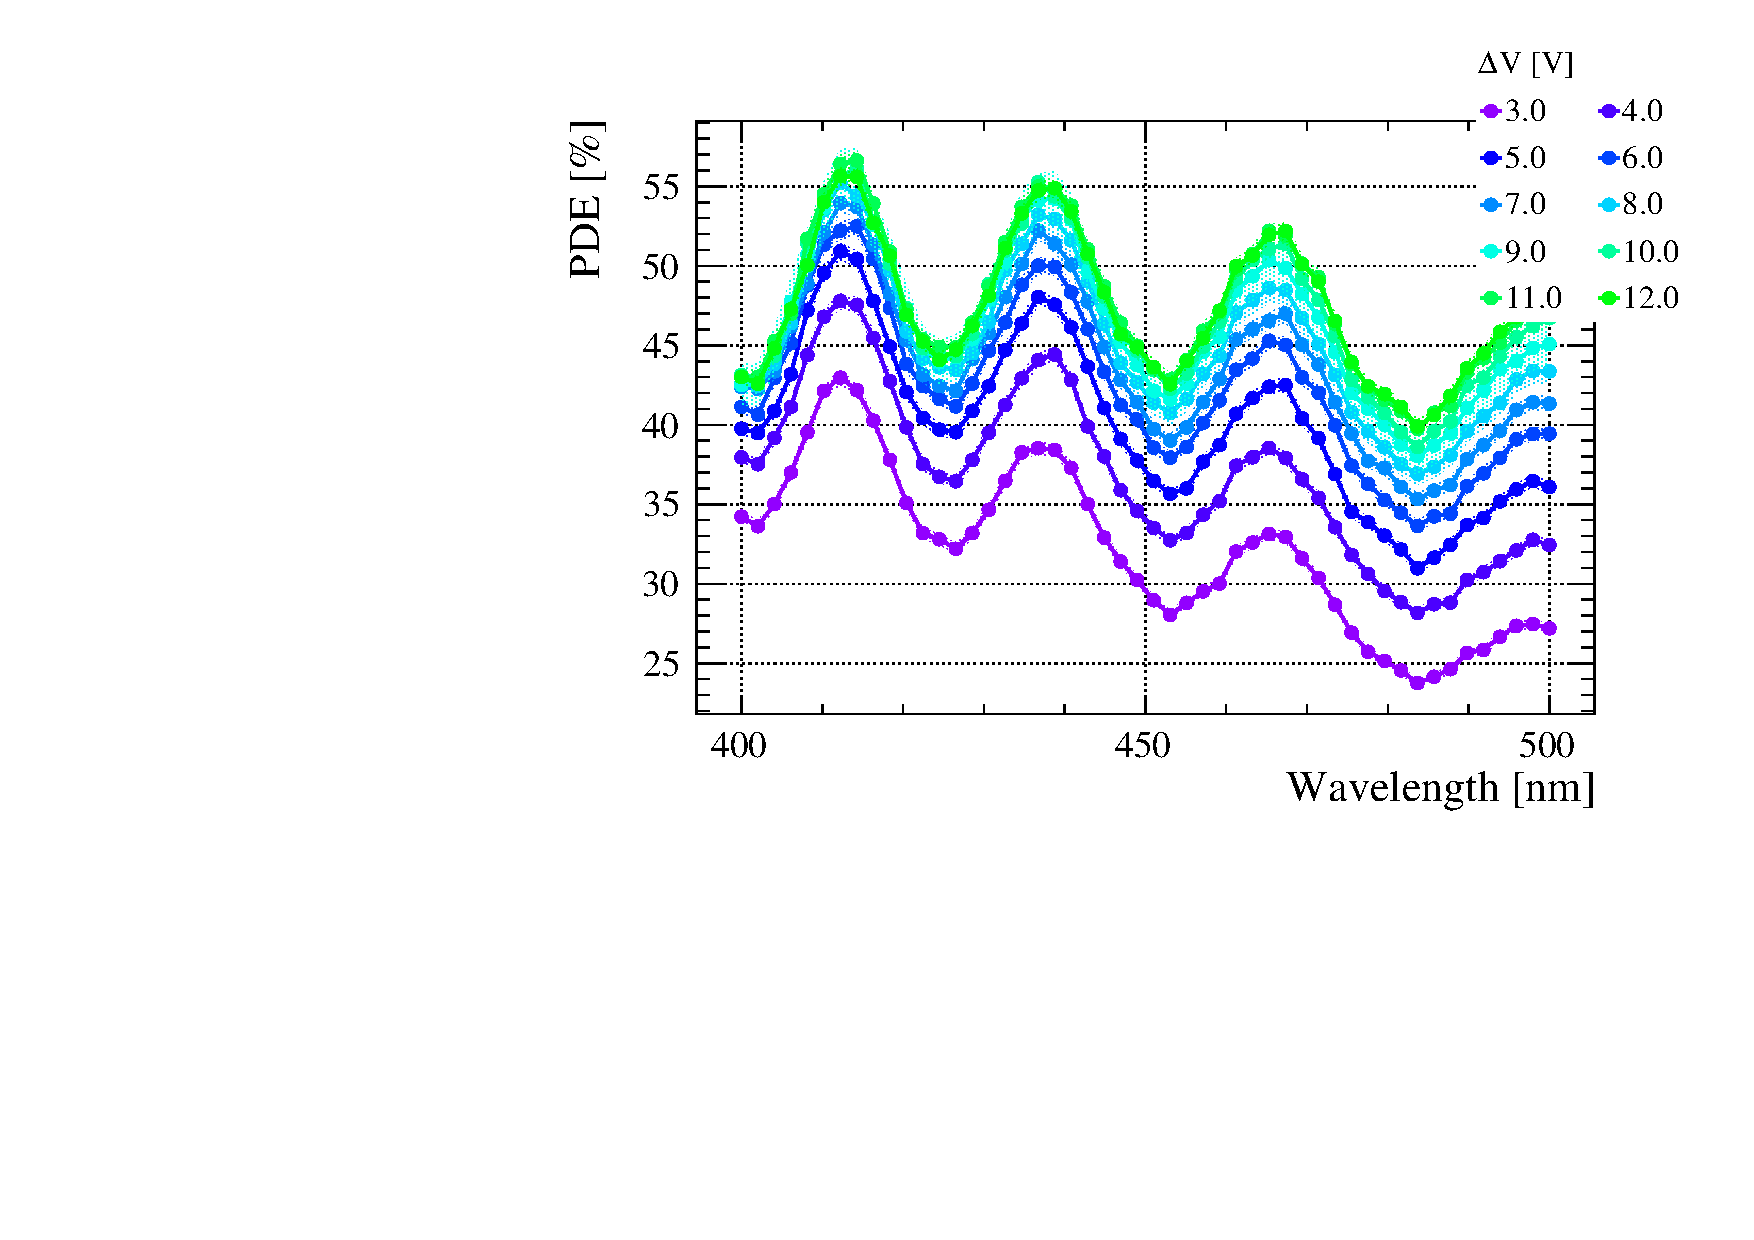
\includegraphics[width=\linewidth]{gfx/plots/PDE/42/c_Freq_Wavelength.pdf} 
        \caption{Rate}
    \end{subfigure}
    \caption{PDE of the FBK \SI{42}{\micro m}. }
    \label{fig:pde 42um}
\end{figure}
\end{landscape}

\begin{landscape}
\begin{figure}[htbp]
    \centering
    \begin{subfigure}{0.65\textwidth}
        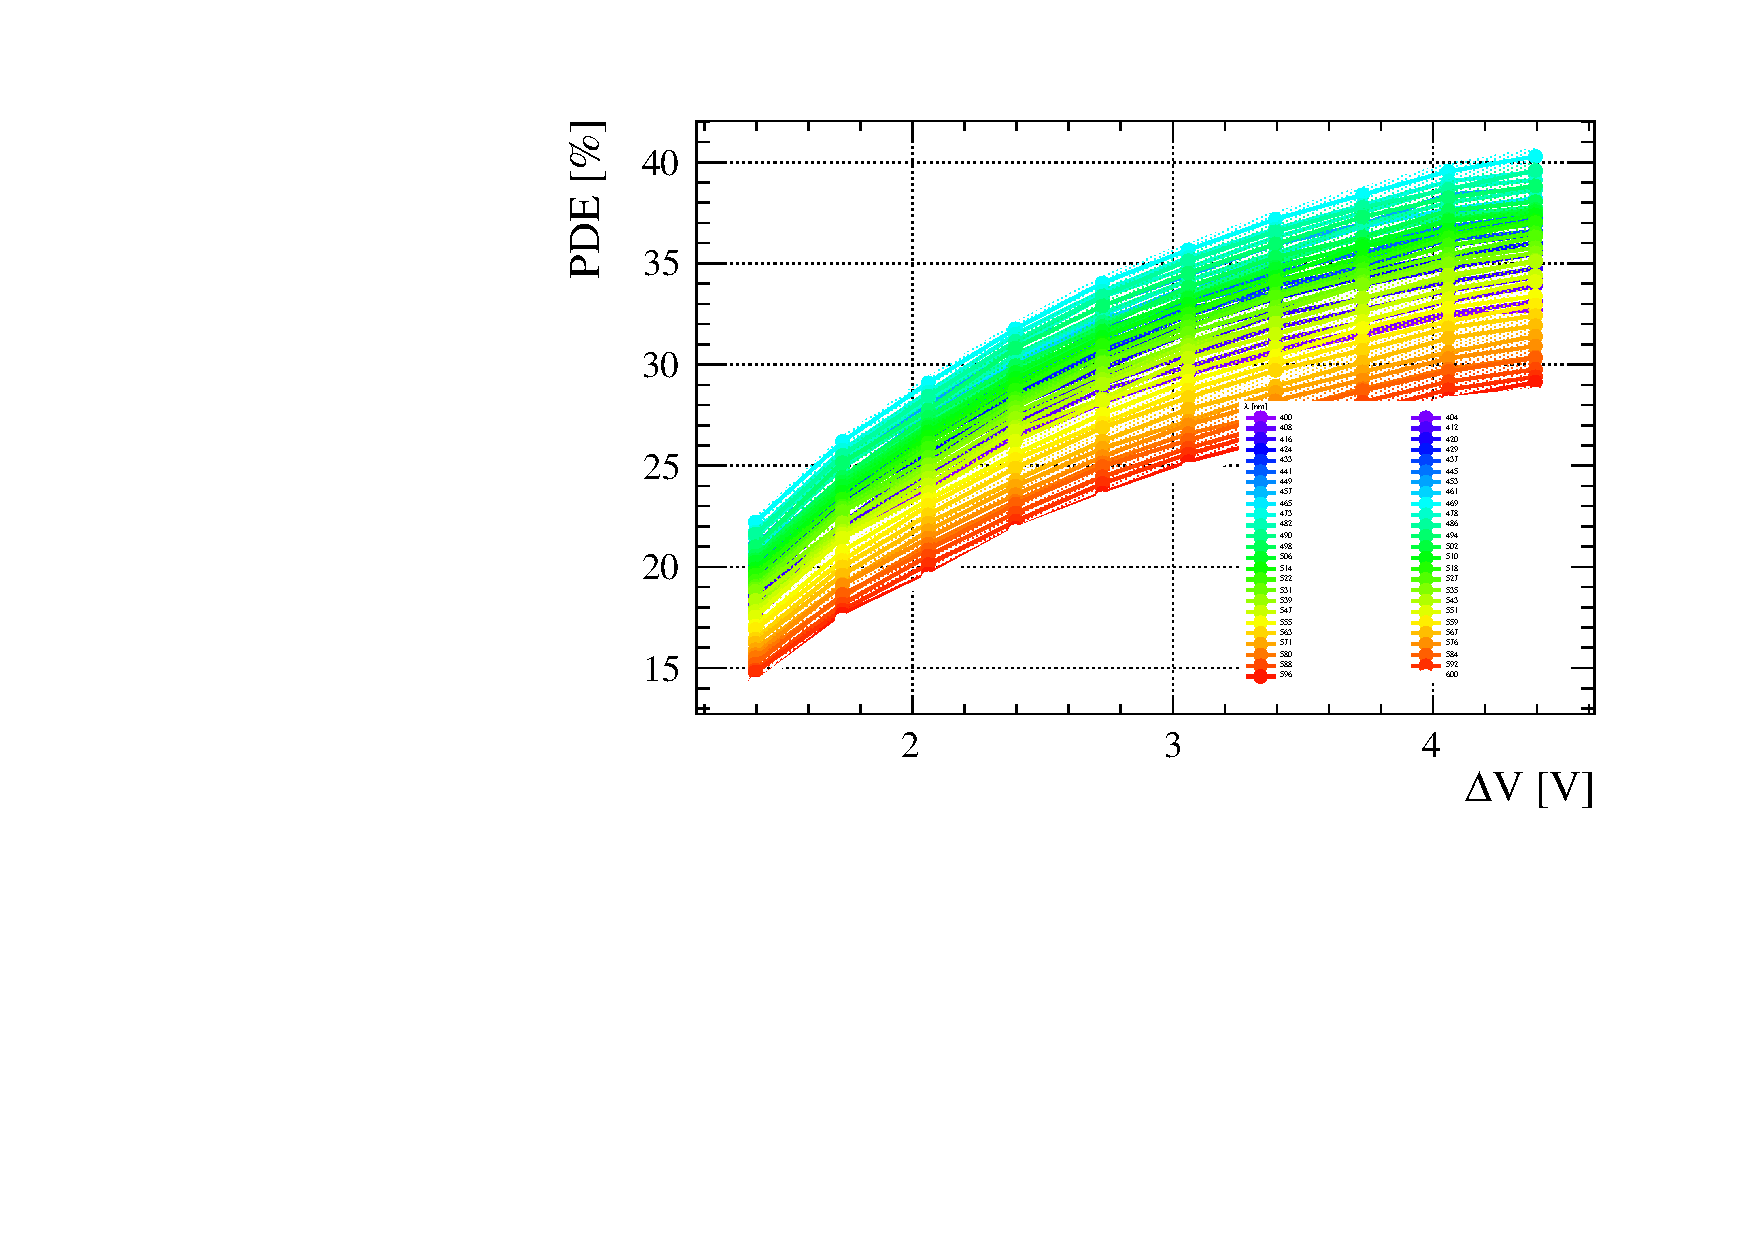
\includegraphics[width=\linewidth]{gfx/plots/PDE/H2017/c_Current_Bias.pdf} 
        \caption{Current}
    \end{subfigure}
    %\hfill
    \begin{subfigure}{0.65\textwidth}
        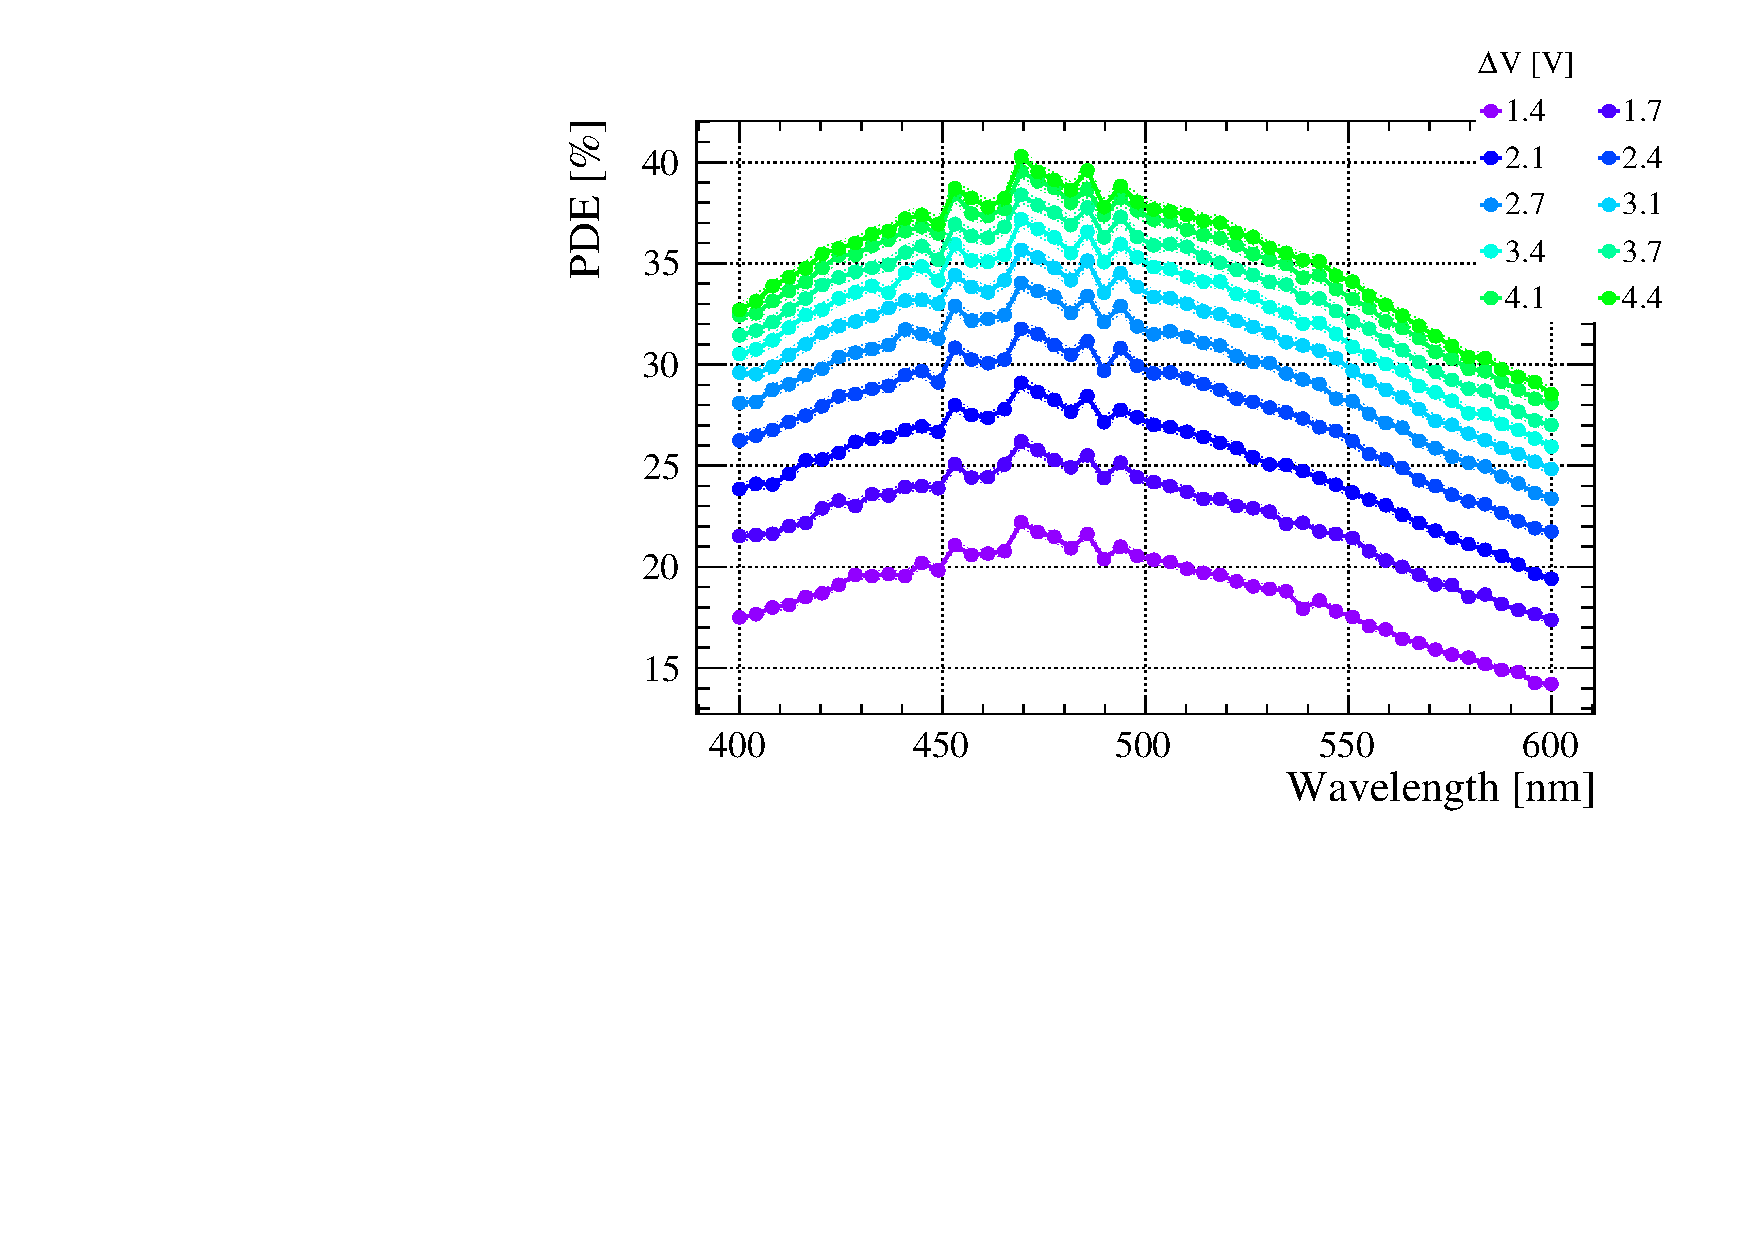
\includegraphics[width=\linewidth]{gfx/plots/PDE/H2017/c_Current_Wavelength.pdf}  
        \caption{Current}
    \end{subfigure}
    \\
    \begin{subfigure}{0.65\textwidth}
        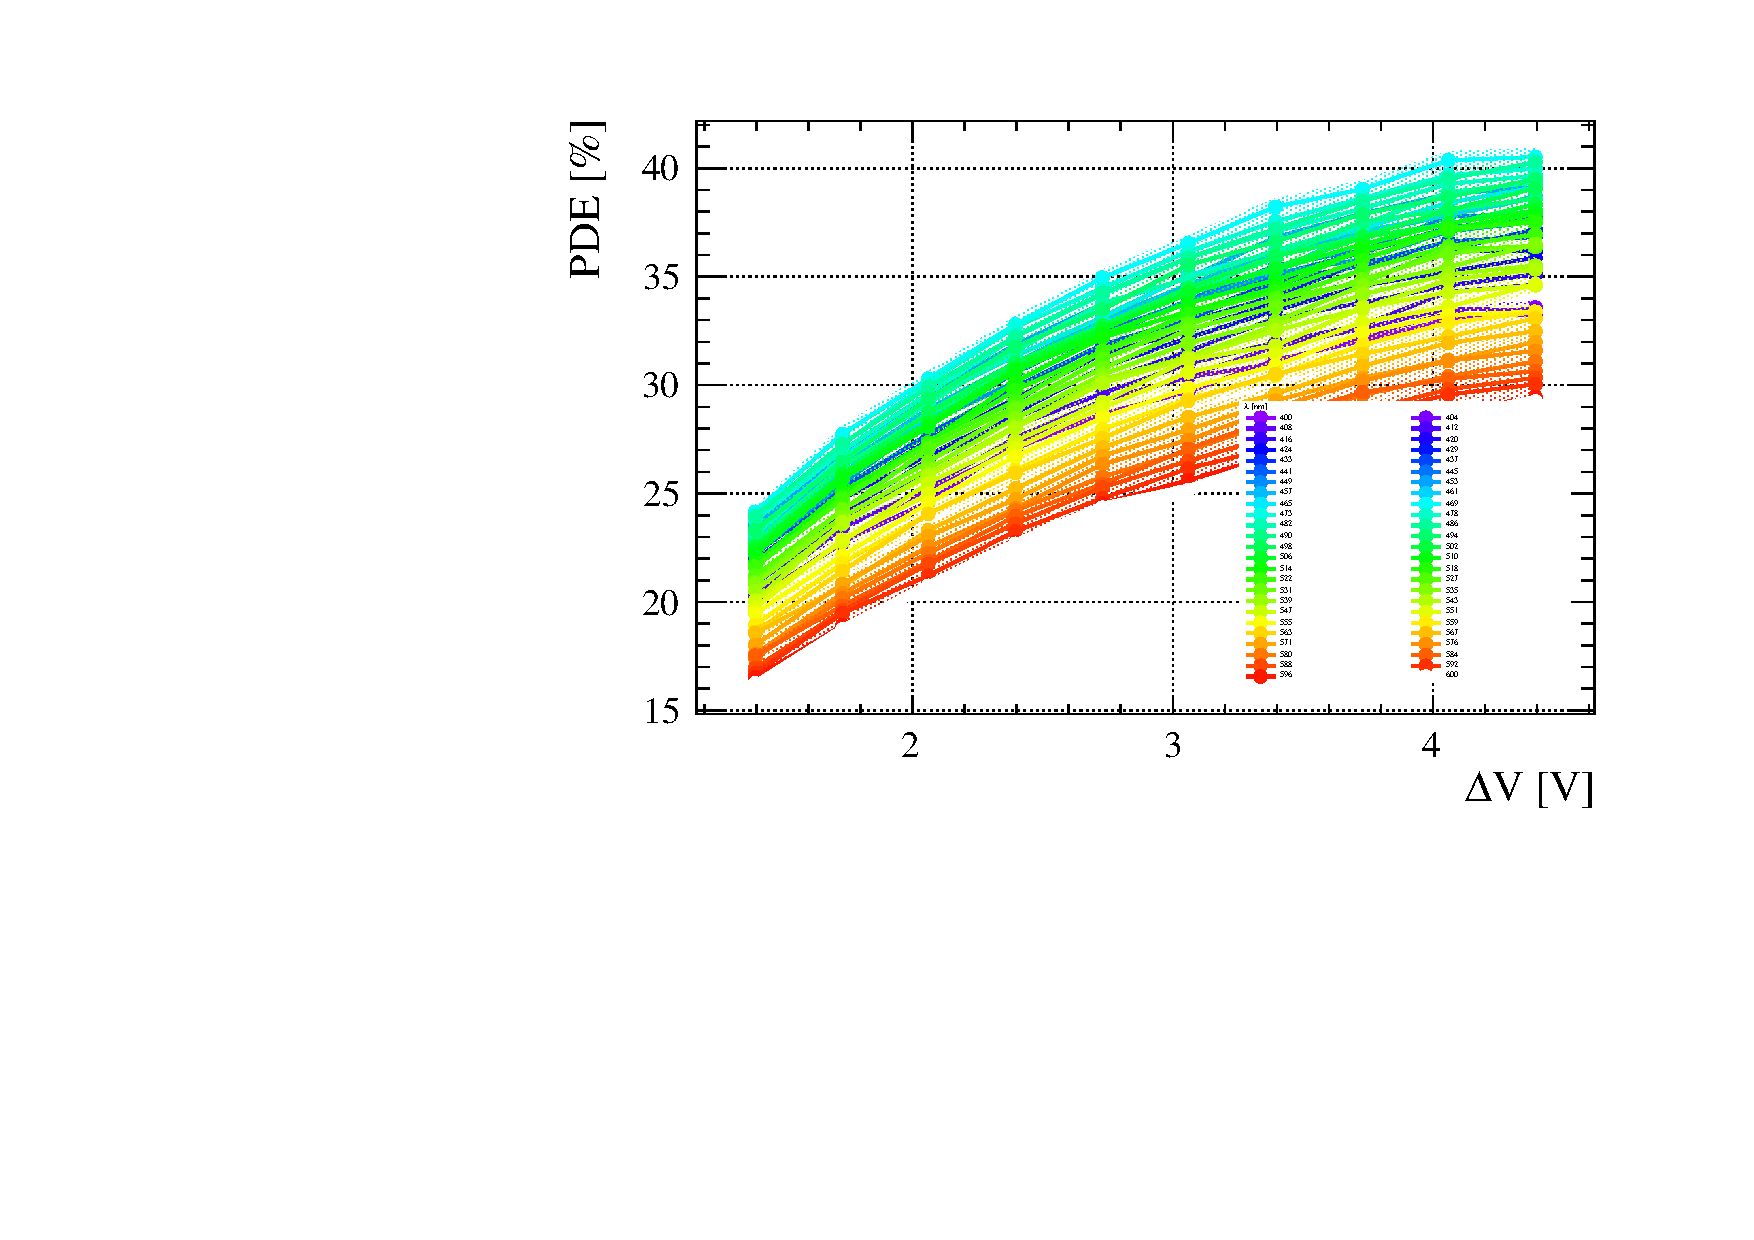
\includegraphics[width=\linewidth]{gfx/plots/PDE/H2017/c_Freq_Bias.pdf}    
        \caption{Rate}
    \end{subfigure}
    %\hfill
    \begin{subfigure}{0.65\textwidth}
        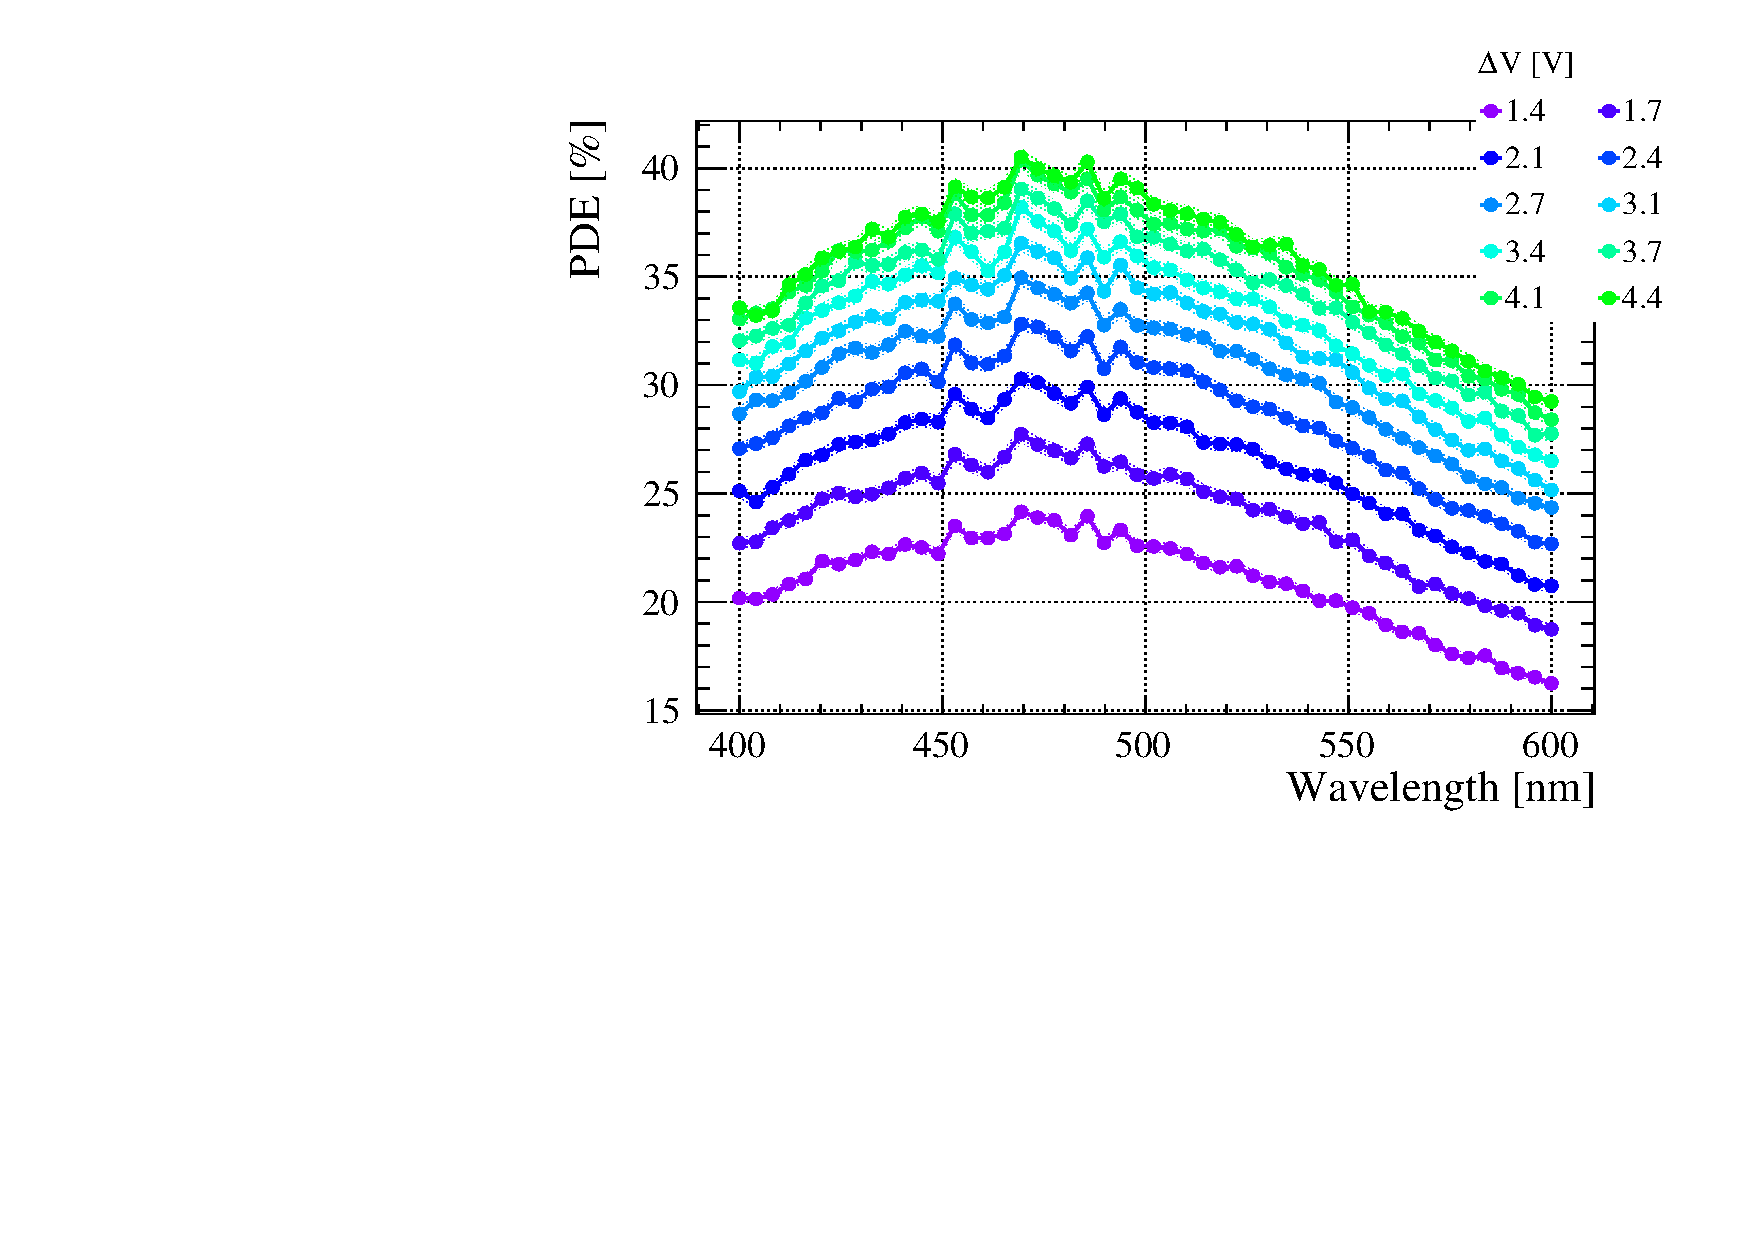
\includegraphics[width=\linewidth]{gfx/plots/PDE/H2017/c_Freq_Wavelength.pdf} 
        \caption{Rate}
    \end{subfigure}
    \caption{PDE of the Hamamatsu H2017.}
    \label{fig:pde H2017}
\end{figure}
\end{landscape}

\begin{landscape}
\begin{figure}[htbp]
    \centering
    \begin{subfigure}{0.65\textwidth}
        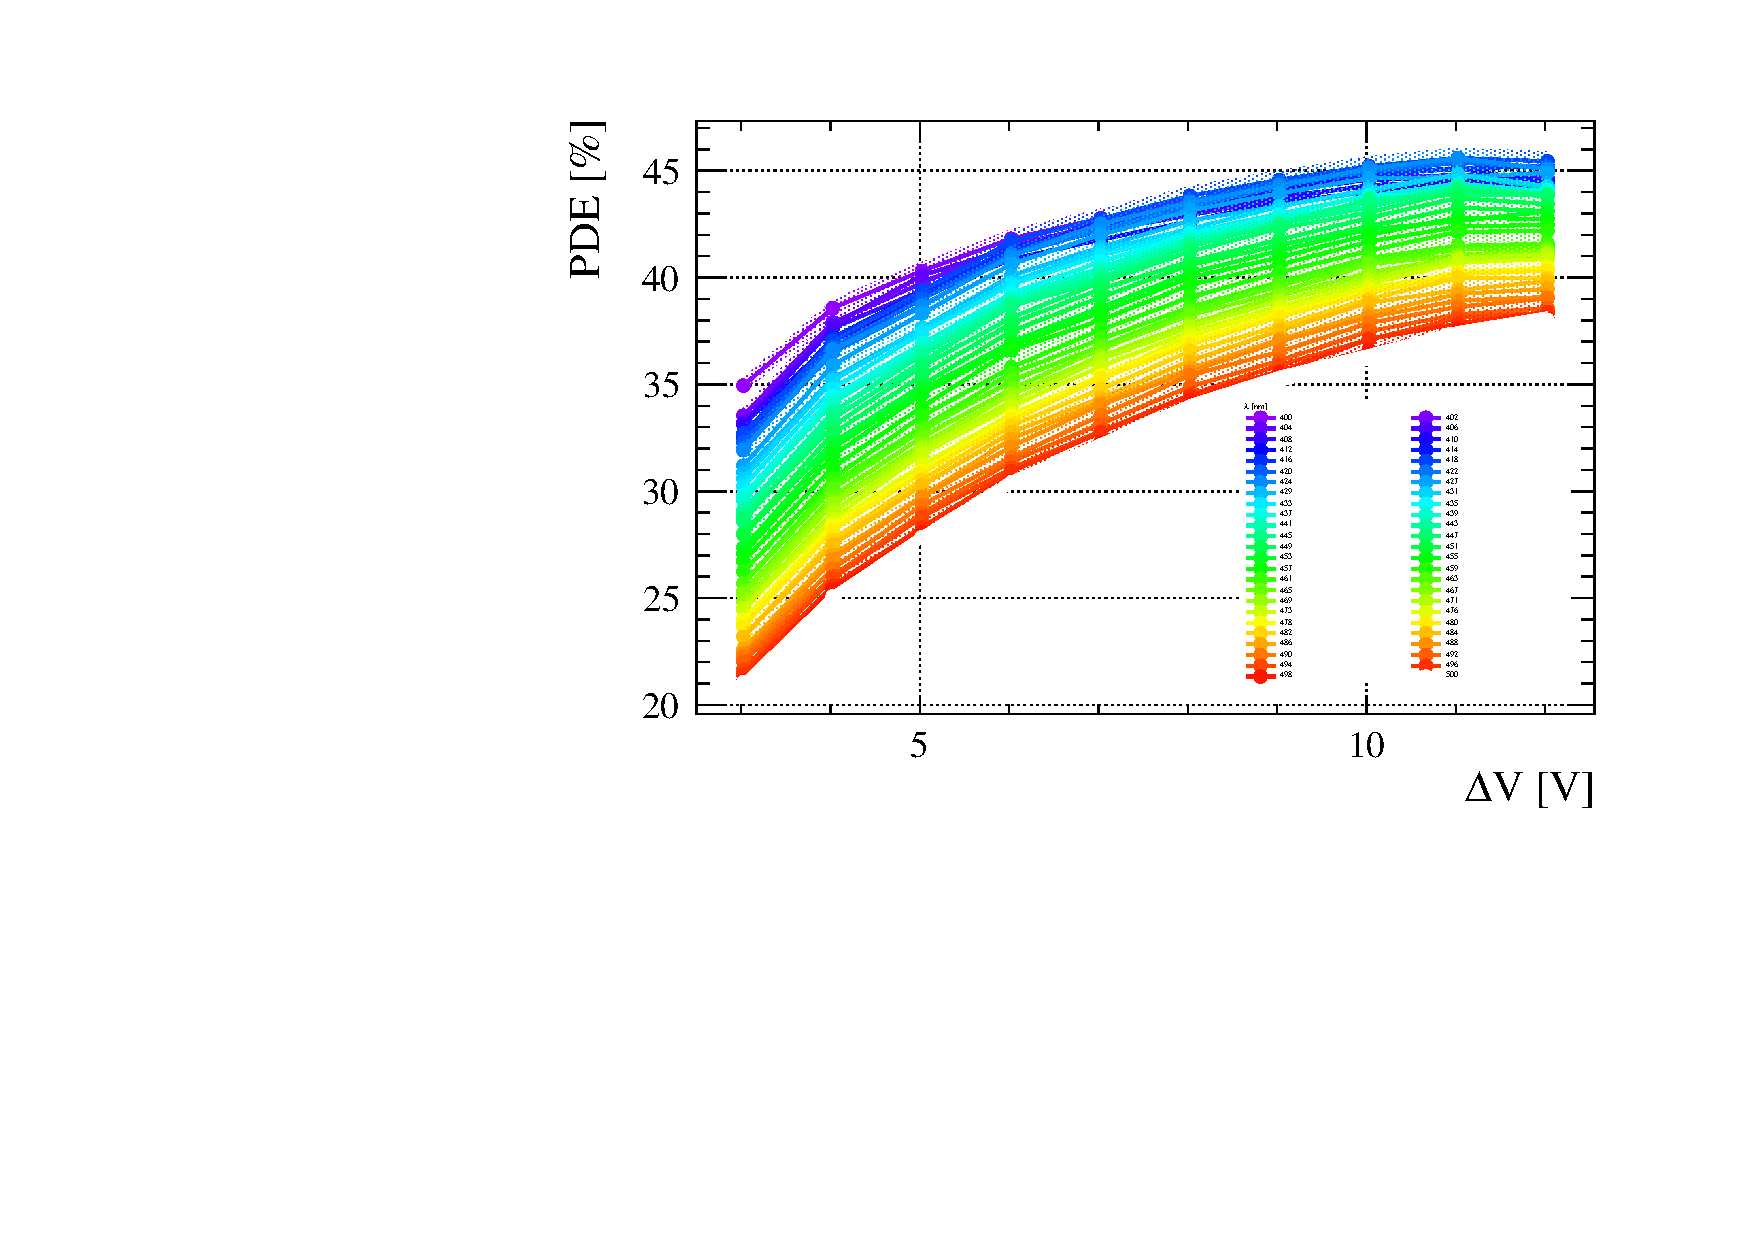
\includegraphics[width=\linewidth]{gfx/plots/PDE/31epoxy/c_Current_Bias.pdf}  
        \caption{Current}
    \end{subfigure}
    %\hfill
    \begin{subfigure}{0.65\textwidth}
        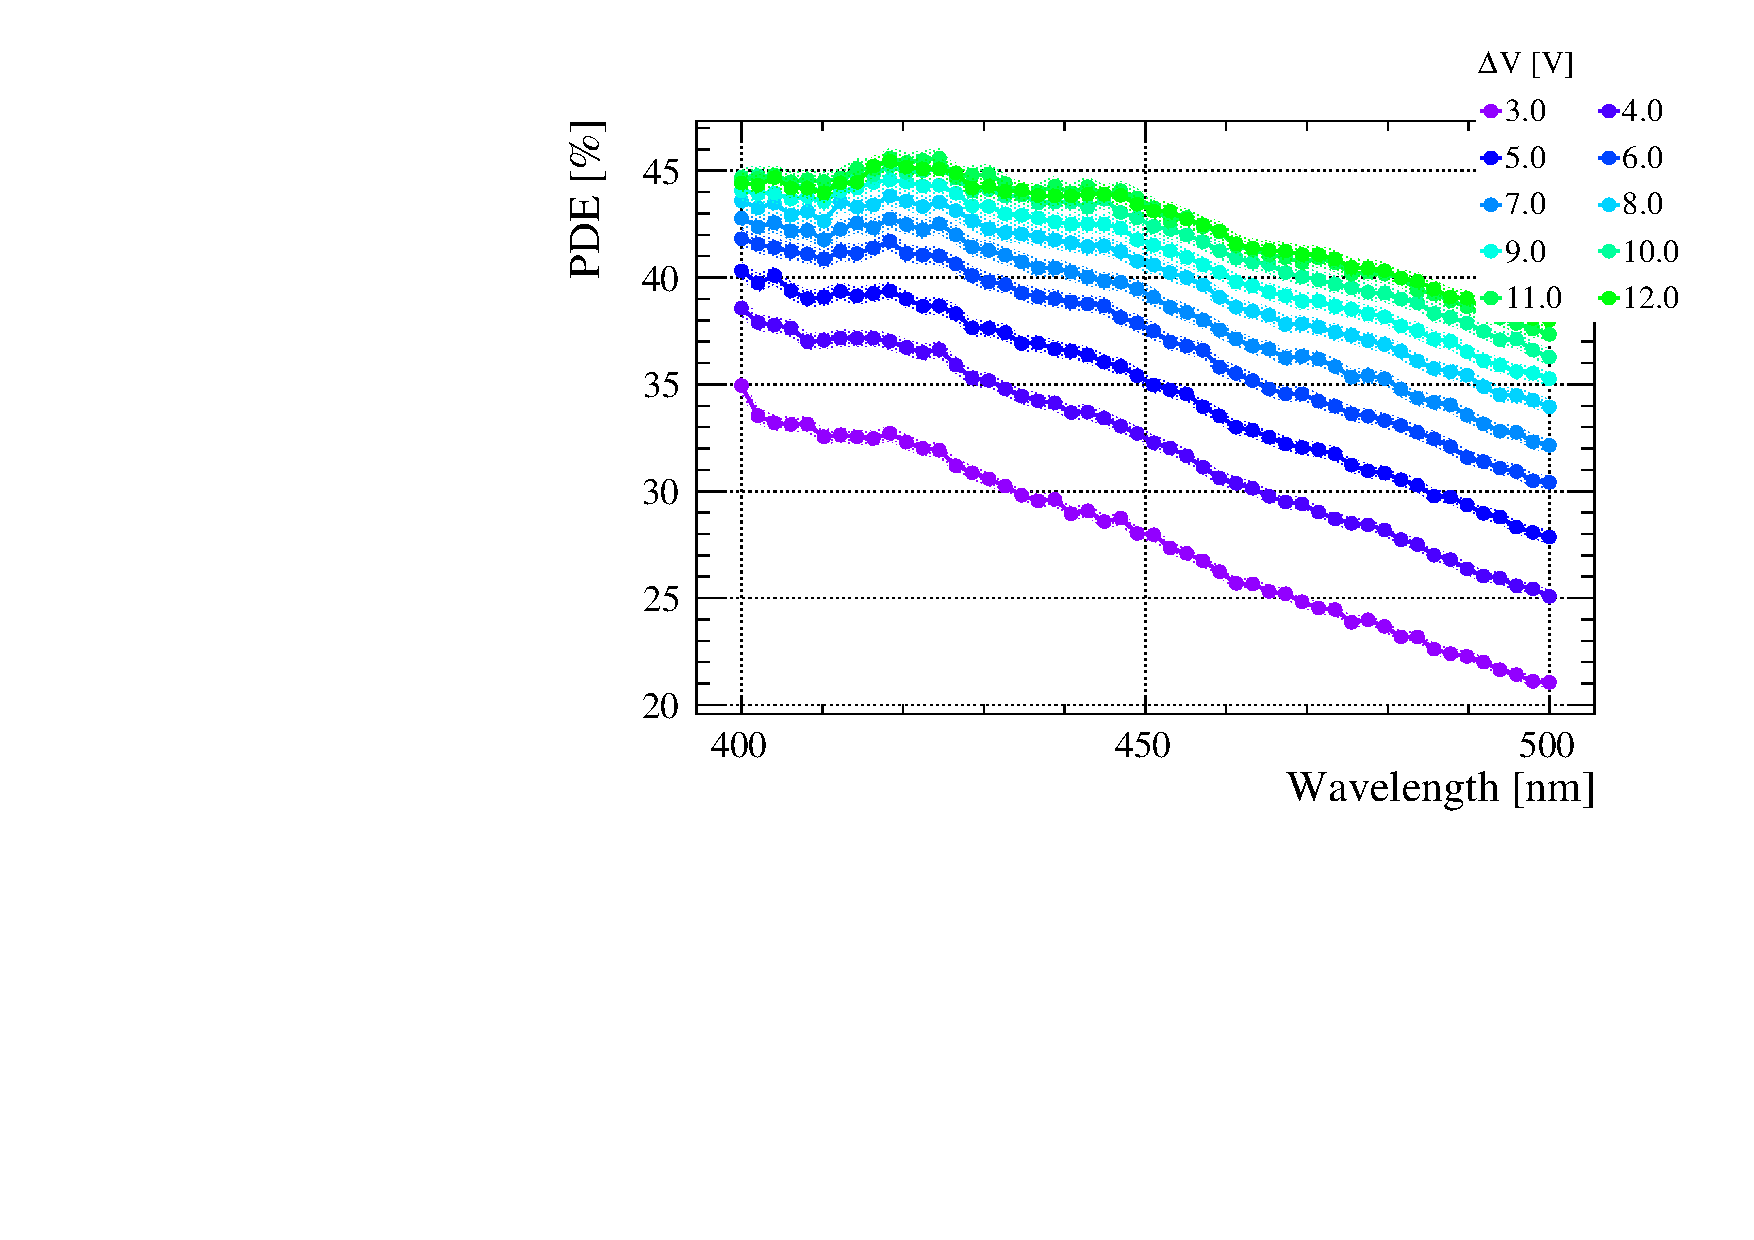
\includegraphics[width=\linewidth]{gfx/plots/PDE/31epoxy/c_Current_Wavelength.pdf}  
        \caption{Current}
    \end{subfigure}
    \\
    \begin{subfigure}{0.65\textwidth}
        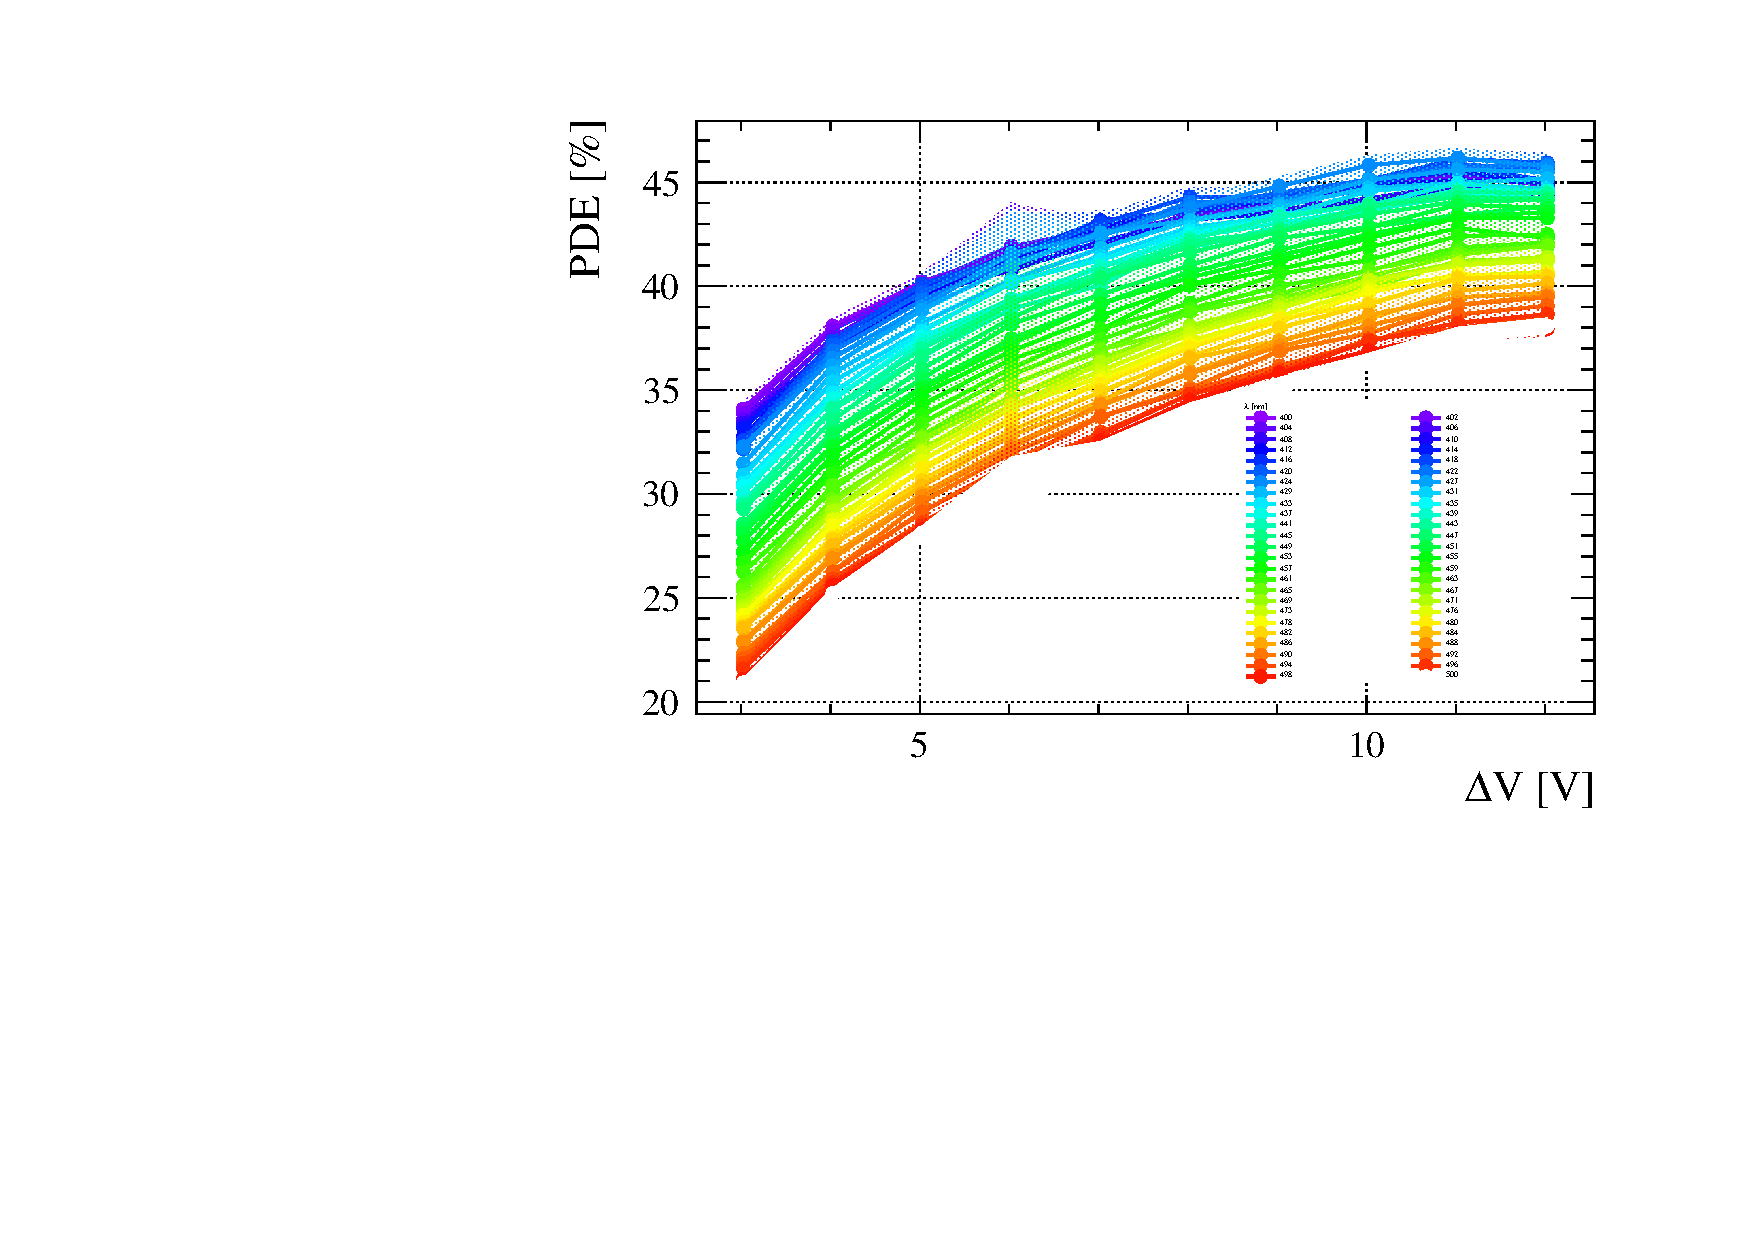
\includegraphics[width=\linewidth]{gfx/plots/PDE/31epoxy/c_Freq_Bias.pdf}    
        \caption{Rate}
    \end{subfigure}
    %\hfill
    \begin{subfigure}{0.65\textwidth}
        \includegraphics[width=\linewidth]{gfx/plots/PDE/31epoxy/c_Freq_Wavelength.pdf} 
        \caption{Rate}
    \end{subfigure}
    \caption{PDE of the FBK \SI{31}{\micro m} + epoxy layer.}
    \label{fig:pde 31epoxy}
\end{figure}
\end{landscape}
\restoregeometry

\begin{figure}[htbp]
    \centering
    \includegraphics[width=0.8\textwidth]{gfx/plots/PDE/PDEcomp.pdf}  
    \caption{PDE of the FBK \SI{31}{\micro m} with and without the epoxy layer at fixed $\Delta V$.}
    \label{fig:pde comp epoxy}
\end{figure}

